\documentclass[type=dr, dr=rernat, accentcolor=tud7b,colorbacktitle, bigchapter, openright, twoside, 12pt ]{tudthesis}
\usepackage[english]{babel} 
\usepackage[utf8]{inputenc}
\usepackage{graphicx}
\usepackage{pstricks}
\usepackage{psfrag}
\usepackage{enumerate}
\usepackage{float}
\usepackage{epsfig}
%\usepackage{geometry}
\usepackage{subfigure}
\usepackage{rotating}
\usepackage{minitoc}
\usepackage{appendix}

%%%% 1 1/2 facher Zeilenabstand:	
\usepackage{setspace}
\onehalfspacing




\begin{document}
\thesistitle{Robust motion mitigation for (noncancerous) lesions in scanned ion beam therapy}{Robuste Methoden zur Verminderung der 
bewegunginduzierten Effekte f\"ur (nicht 
kanzer\"ose) L\"asionen in der Therapie mit nachgef\"uhrten Ionenstrahlen}
\author{MSc Anna Maria Constantinescu}
\birthplace{Bukarest, Rum\"anien}
\date{\today}
\referee{Prof. Dr. Marco Durante}{Dr. Christoph Bert}
\department{Fachbereich Physik}
\group{Prof. Durante\newline Institut f\"ur Festk\"orperphysik}
\dateofexam{}{}
\makethesistitle


\affidavit{Anna Constantinescu}

% % \dominitoc \tableofcontents
% % \dominilof \listoffigures

\dominitoc

% in big toc display only chapters and sections
\setcounter{tocdepth}{1}
\tableofcontents

\chapter{Introduction}
\minitoc
% \minitoc \mtcskip \minilof 

Radiosurgery has the potential to become a new and non-invasive treatment modality for the most common cardiac arrhythmia, atrial fibrillation. 
Irradiation with photons are known to alter the electrical pathway of the heart's conduction system \cite{Sha10}. Based on the 
experience gained in cancer radiotherapy promising results are expected by the usage of scanned carbon ion beams. In order to explain the 
underlying physical and biological differences between carbon ions and photons as well as other ions (e.g. protons), and the resultant benefits 
of carbon ions when irradiating a deep seated target, the physical and radiobiological fundamentals will be explained in the first section of 
this chapter. Furthermore the difference in radiotherapy application will be outlined in the second section, with special emphasis on the 
irradiation of moving targets. In the last subsection the basics of the heart's conduction system will be presented. Abnormalities, risk 
factors and underlying mechanisms causing cardiac arrhythmia in general and especially atrial fibrillation will be explained. The currently 
existing treatment modalities for atrial fibrillation, as well as their limitations and risk factors will be presented in order to motivate 
the benefits of a non-invasive treatment modality. 

%%%%%%%%%%%%%%%%%%%%%%%%%%%%%%%%%%%%%%%%%%%%%%%%%%%%%%%%%%%%%%%%%%%%%%%%%%%%%%%%%%%%

\section{Physical and biological basics of radiotherapy}
\label{pbb}
The usage of radiation for medical purposes is almost as old as its detection. Shortly after W.C. Roentgen discovered X-rays in 1895 it 
was first used for the treatment of a cancer patient \cite{Hal06}. With the development of accelerators and the resulting study of ion 
energy deposition profiles particles were almost immediately connected to their therapeutic implications and benefits 
\cite{Wil46}. In the following the physical and biological fundamentals of radiotherapy will be presented.


\subsection{Dose}

The dose $D$ is defined as the deposited energy per unit mass \cite{ICRU93}:

\begin{equation}
 D = \frac{dE}{dm} ; \hspace{0.4cm} [D]= 1 Gy = 1 \frac{J}{kg}
 \label{dose}
\end{equation}

The magnitude of the deposited dose in an material depends, among other factors, on the used particle type, as they underlie different 
physical interaction mechanisms, which will be explained in the following. 


\subsection{Interaction of radiation with matter}

Photons and ions interact differently with matter, resulting in different depth-dose-profiles (see figure \ref{ddp}). While photons deposit 
their highest local dose shortly after entering the material, ions display an inverse depth-dose-profile. Thereby most of their energy 
is deposited in a defined area at the end of the particle track, the so-called Bragg Peak region, which is beneficial when irradiating a 
deep seated target as the dose to the surrounding healthy tissue can be drastically reduced. Even though the interaction 
mechanisms for the energy deposition of photons and ions occurs primarily through secondary electrons, the underlying processes 
differ.

\newpage
 
\vspace*{1cm}
 
\begin{figure}[H]
\begin{center}
% 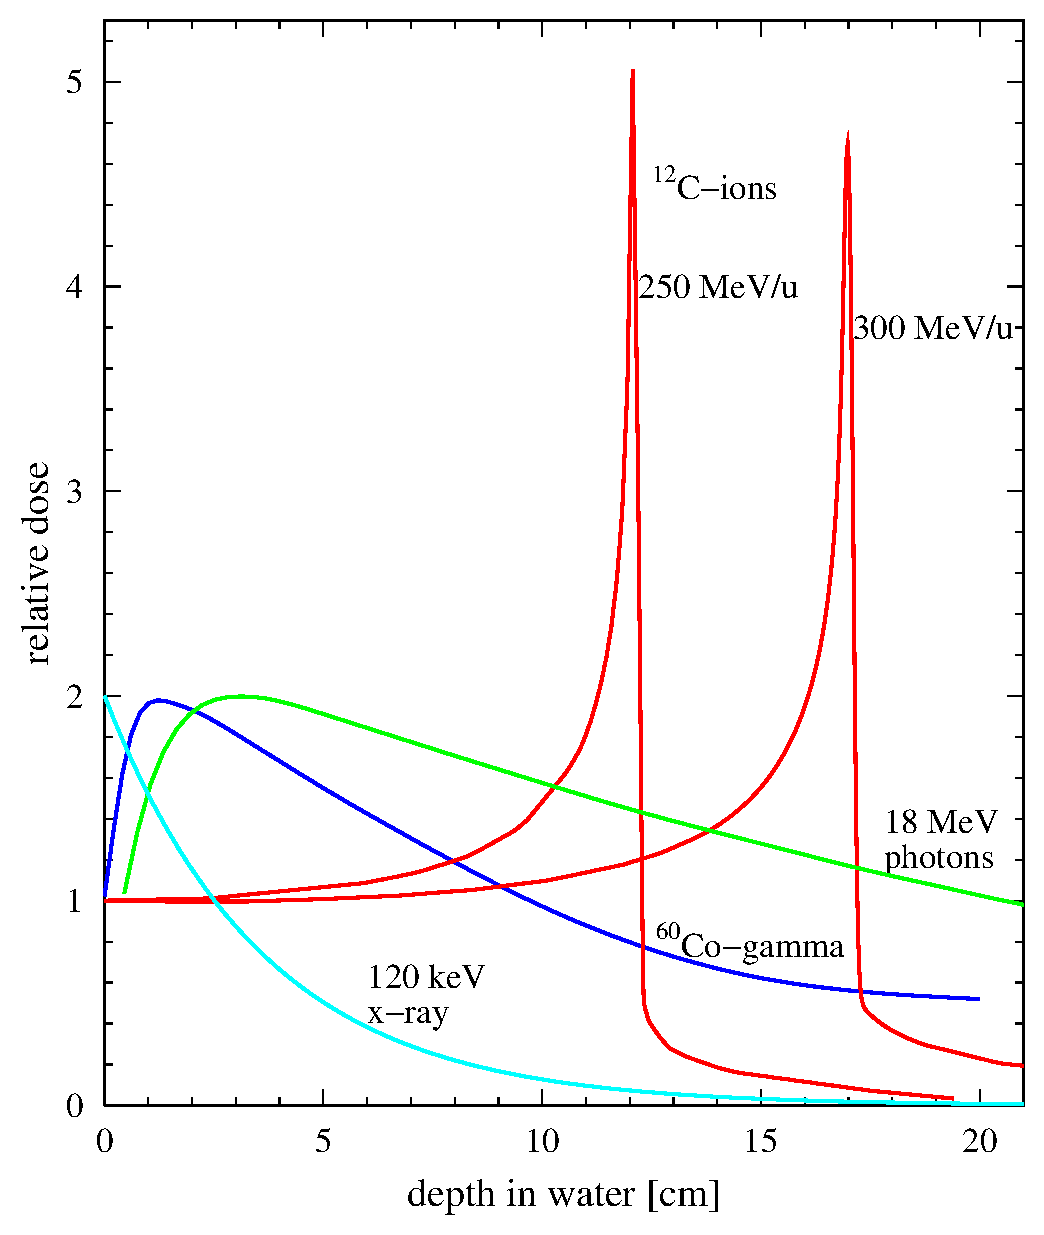
\includegraphics[scale=1]{depthdose.eps}
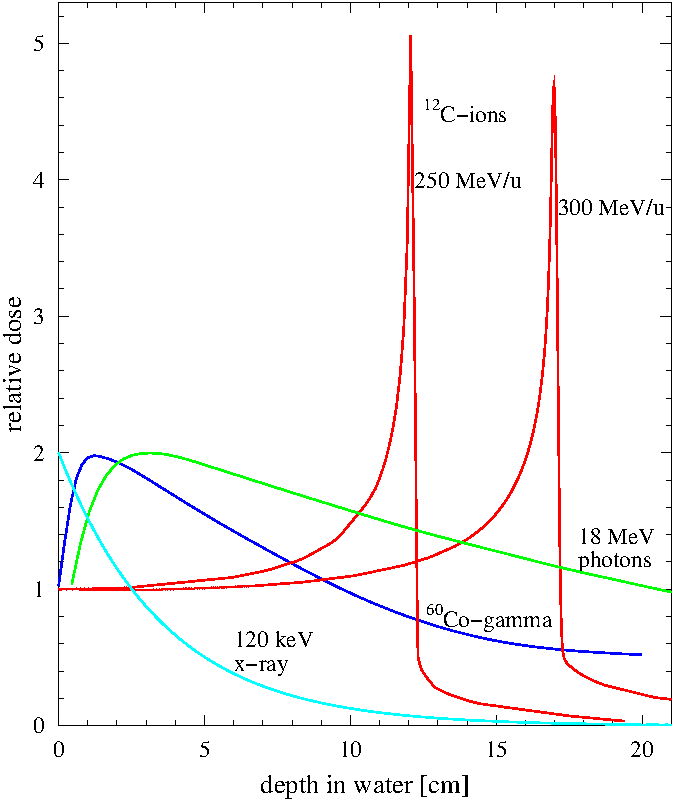
\includegraphics[scale=1]{depthdose.png}
\caption{Depth dose distributions of photons and carbon ions at different energies. Photons display an exponential decrease after a certain 
build up. Ions on the other hand interact differently with matter, resulting in an increased dose deposition at the end of the particle 
track, the Bragg peak. Figure taken from \cite{Lue12}}
\label{ddp}
\end{center}
\end{figure}
% \newpage

\subsubsection{Interaction of photons with matter}

Photons undergo different processes when passing matter, like coherent scattering or Rayleigh scattering, photoelectric effect, Compton 
scattering and pair production. The probability for each process depends on one hand on the energy of the primary photons as well as on the 
atomic number of the absorbing material, while the strength of these dependencies varies in turn on the different processes \cite{Lil06}. 
The overall decrease of the photon beam intensity when passing a material can be described by the following formula:

\begin{equation}
 I = I_{0} \cdot e^{- N \sigma x} = I_{0} \cdot e^{-\mu x}
 \label{expdecrease}
\end{equation} 

where $I_{0}$ represents the intensity of the incident photon, $x$ the depth of the material in units of length, $N$ the atomic density 
of the material and $\mu$ is the attenuation coefficient. The latter is directly related to the overall cross section $\sigma$, which is a 
measure of the probability of the occurrence of an interaction mechanism. It has contributions from all single interaction processes. 

\begin{equation}
{\sigma} = \sigma_{rayleigh} + \sigma_{photoelectric} + Z\sigma_{compton} + \sigma_{pairproduction} 
\end{equation}

In the energy range of radiotherapy (between 100 keV and 10 MeV) the dominating process is Compton scattering \cite{Alp98}. 
The attenuation of the photon beam results thus in the following way: 
The Compton electrons are scattered in a strongly forward direction, leading to a build up effect in deeper layers of the material. The 
maximum of the depth-dose profile is reached when the electrons are completely stopped at a certain depth, which is called the mean electron 
range (and is dependent on the initial photon energy). Afterwards the dose deposition decreases exponentially (see eq. \ref{expdecrease}). 

% in which the photons induce electron oscillation in the medium, causing the emission of a photon with the same energy but other direction as the primary photon. 

\subsubsection{Interaction of ions with matter}

Interaction of ions with matter occurs via one of the following processes: elastic coloumb scattering from target nuclei (nuclear stopping) 
and inelastic collision with target electrons (electronic stopping). In the mildly relativistic region used in radiotherapy 
(energies of less than 500 $\mathrm{MeV}/\mathrm{u}$) the total stopping power of ions is dominated by electronic stopping, 
resulting in ionization and excitation of the target atoms. 
% At very small ion energies, e.g. at the end of the particle range, nuclear stopping start to contribute to the total energy loss. 
% The mean rate of energy loss is described in the Bethe formula \cite{Bet30} \cite{Blo33}:
The Bethe-Bloch formula \cite{Bet30} \cite{Blo33}, describing the mean rate of energy loss of relativistic ions, can thus be corrected 
for low particle energies \cite{Nak10}, resulting in the following approximation:

\begin{equation}
- \left \langle \frac{dE}{dx} \right \rangle = \frac{ 4 \pi N_{e} z_{eff}^{2} }{ m_{e} v^{2} } \left( \frac{e^{2}}{4\pi \epsilon_{0}} \right) ^{2} \left[ln \left( \frac{2m_{e}v^{2}}{I} \right)+correction \right]
 \label{bethe}
\end{equation}

where $N_{e}$ is the materials electron density, $e$ and $m_{e}$ are the charge and mass 
of an electron, $\epsilon_{0}$ the electrical field constant and $I$ the mean excitation energy of the absorber material. The effective 
projectile charge $z_{eff}$ can be approximated by the Barkas formula \cite{Bar63}, where $\beta$ is the projectile speed in units of 
$c$: 

\vspace*{-0.8cm}
\begin{equation}
 z_{eff} = z \left( 1 - e^{-125 \beta z^{\frac{2}{3}}} \right)
\end{equation}

The main dependencies of the mean rate of energy loss can be seen in equation \ref{bethe}. It is proportional to $z_{eff}$ 
and inversely proportional to $v^{2}$. The overall depth dose distribution can thus be understood in the following way: in the beginning 
the particles have a high energy and thus high velocity, causing the dose deposition to be small. While passing the material, the velocity 
of the projectile decreases, causing the energy deposition to increase. At low particle energies, close to the particle range, 
target electrons are collected hence causing $z_{eff}$ to decrease, leading to a decrease in dose deposition. This leads to a maximum 
energy loss around the particle range, known as Bragg peak. 

\subsubsection{Range straggling and lateral scattering}
\label{scat}
Even though electronic stopping via inelastic collisions with target electrons is the main interaction process in the therapeutic energy 
range, elastic Coulomb scattering from target nuclei is still occurring and the main reason for lateral scattering. In an analytical 
approximation by Moli\`{e}re \cite{Mol48}, the angular spread of the overall deflection in a material has been described. It is 
on the one hand dependent on the mass of the target nuclei, where a higher mass causes a larger angular spread for the same thickness 
of material. And on the other hand it is inversely proportional on the momentum of the projectile, causing carbon ions to have a smaller 
lateral deflection than e.g. protons. Experimental validation comparing carbon ions to protons having the same range in water 
(15.6 cm, 150 MeV protons and 285 MeV/u 12C ions) resulted in an approximately three times smaller angular spread \cite{Sch10}.\newline
\newline
Range straggling is caused by the statistical fluctuations of single electronic stopping events. In case of large number of collisions or 
thick layers of material these fluctuations can be approximated by a Gaussian probability distribution \cite{Bor40} 
\cite{Ahl80} \cite{Ric12}. This leads to an inverse proportional dependence between the ratio of the straggling width $\sigma_{R}$ with 
the mean range $R$ and the square root of the ion mass $M$ ( $\mathrm{\sigma_{R}}/\mathrm{R} \propto \mathrm{1}/{\sqrt{M}}$ ). This results 
in a smaller range scattering for heavier ions. Experimentally, the ratio between the straggling width and the mean range was found to be 
3.5 smaller for carbon ions compared to protons \cite{Sch10}.
%%% XXX FIGURE LATERAL SCATTERING SCHARDT10 ?


\subsubsection{Nuclear fragmentation}

At large penetration depths, when the projectile ions have lost most of their energy, nuclear fragmentation processes start to be 
relevant for all ions heavier than protons. Mostly lower Z fragments are produced, which move with approximately the same velocity 
and in the same direction as the primary ions. This causes dose tails behind the Bragg peak position. Thus the resulting depth-dose 
distribution for all ions heavier than protons is actually the sum of the energy deposition of the projectiles and the resulting 
fragments. 

\begin{figure}[H]
\begin{center}
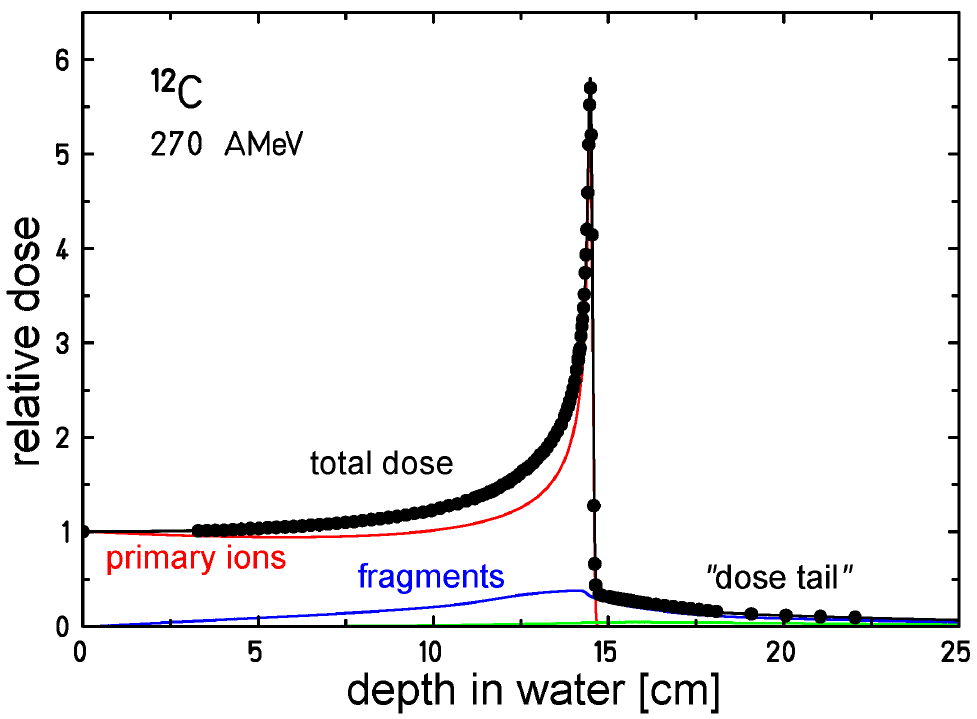
\includegraphics[scale=0.3]{iondepthdosesum.png}
\caption{Depth dose distribution of carbon ions. Besides of the energy deposition of the primary ions (red), the produced fragments 
(blue curve) contribute to the overall dose deposition (black) and are especially visible in the dose tail behind the Bragg 
peak. Figure taken from \cite{Gro04}}
\end{center}
\end{figure}

In case of carbon ions, the produced fragments nevertheless also offer the chance for PET (Positron Emission Tomography) monitoring, 
without additional radiation exposure for the patient. As peripheral collisions are more frequent then central ones \cite{Kra00} 
isotopes like $^{11}C$ and $^{10}C$ are produced when $^{12}C$ ions penetrate through tissue. Both isotopes are $\beta^{+}$ 
emitters. They annihilate with electrons in the human body, producing two $\gamma$-rays which travel in opposite directions.

% \newpage

\subsubsection{Track structure}

For inelastic collisions with atomic target electrons, only about 20\% of the initial projectile energy is used to overcome the 
electron binding energy \cite{Kra92}. A high amount of energy is transformed into the kinetic energy of the secondary electrons, the 
so-called $\delta$-electrons. These $\delta$-electrons can in turn emerge from the primary particle trajectory and undergo frequent 
elastic and inelastic scattering. If their energy is sufficient high they can induce further ionization in more distant locations, 
leading to a high number of additional electrons. The radial dose fall off is approximated by a $\mathrm{1}/\mathrm{r^{2}}$ law, 
illustrating that the radial dose quickly falls off with larger radial distance $r$ \cite{Cha76} \cite{Kat99} \cite{Ric12}. 
The range of the $\delta$-electrons is restricted to a maximum value according to the kinematics of the collision between projectile 
and target electron. Empirically this can be described by a power law \cite{Kie86}, where $E$ is energy of the primary ion:

\begin{equation}
 r_{max} \propto E^{1.7}
\end{equation}

As stated by the Bethe equation \ref{bethe}, the energy deposition of the primary ions is dependent on the used ion species and their 
energy. This results in a higher stopping power for higher $Z$ primary ions as well as an increased stopping power for smaller energies. 
Hence carbon ions have a much higher $\delta$-electron output than e.g. protons. Furthermore with decreasing energy of 
carbon ions, the $\delta$-electron output increases. This can be seen in figure \ref{track}. This difference in $\delta$-electron output 
is also the reason for the difference in induced biological damage. 

\subsubsection{Linear Energy Transfer LET}

The criteria for the occurrence of direct or indirect actions causing DNA damage is dependent on the local energy deposition pattern. 
The critical measure for this is the linear energy transfer (LET). It is defined as the average energy deposited per unit length of track 
\cite{Hal06} and is typically given in keV/$\mu$m. Indirect actions are caused by radiation with a low LET (sparsely ionizing), 
such as photons, protons and fast ions. Direct actions are caused by high LET radiation (densely ionizing), such as slow ions. 

\newpage

\vspace*{1cm}

\begin{figure}[H]
\begin{center}
% 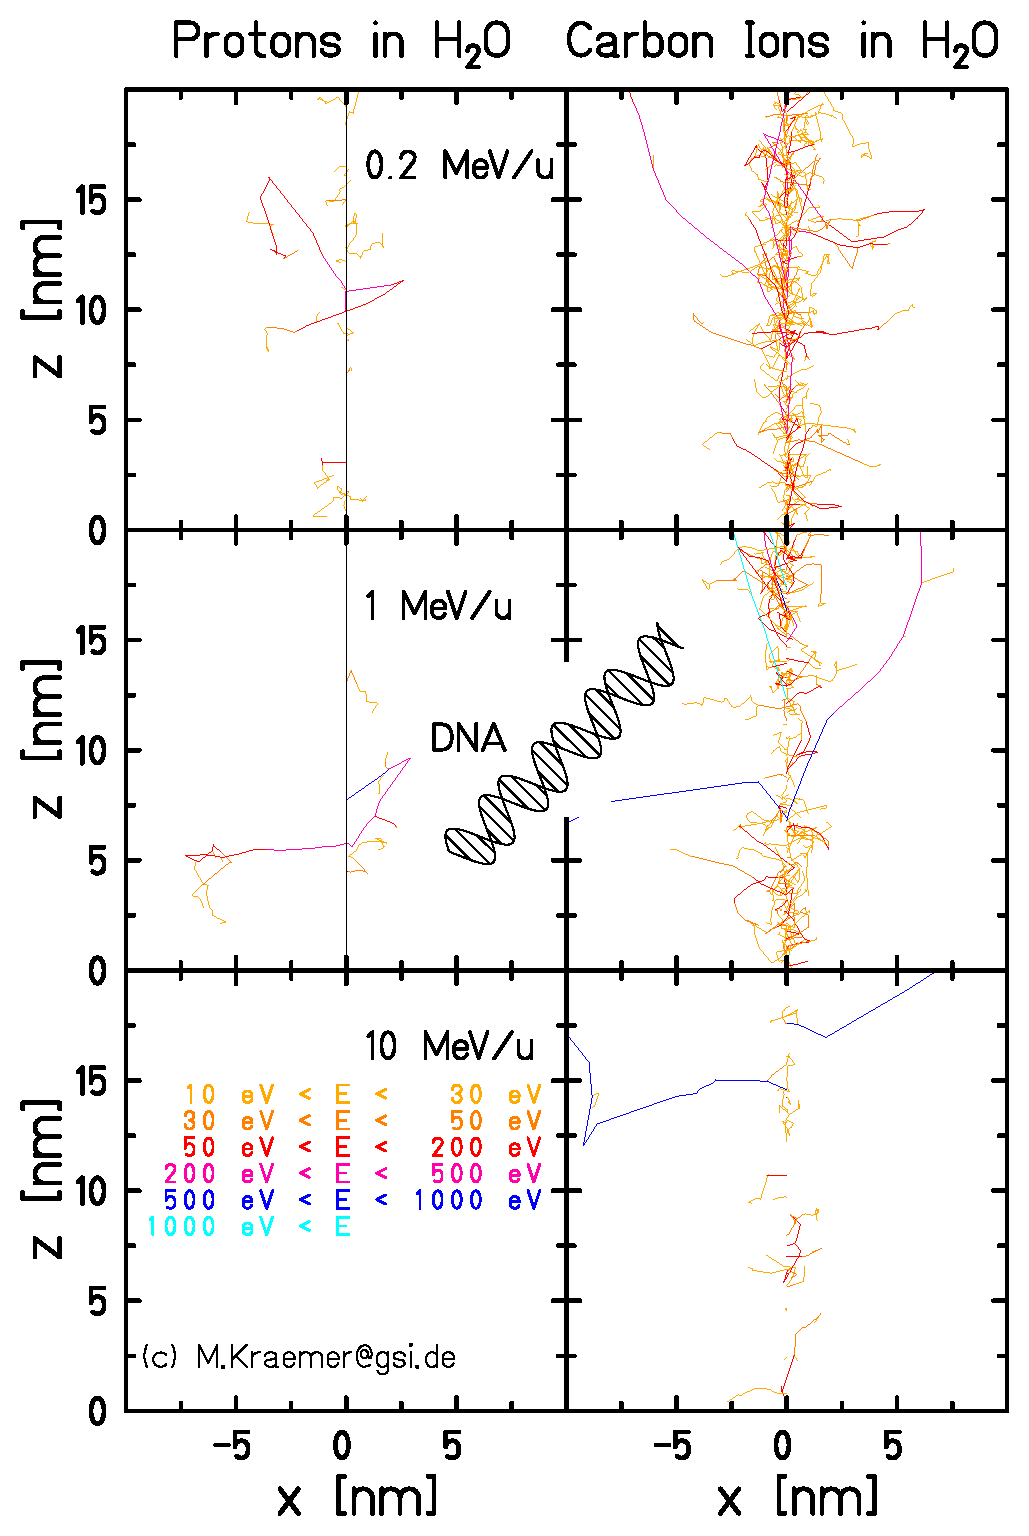
\includegraphics[scale=0.75]{trackstructure.eps}
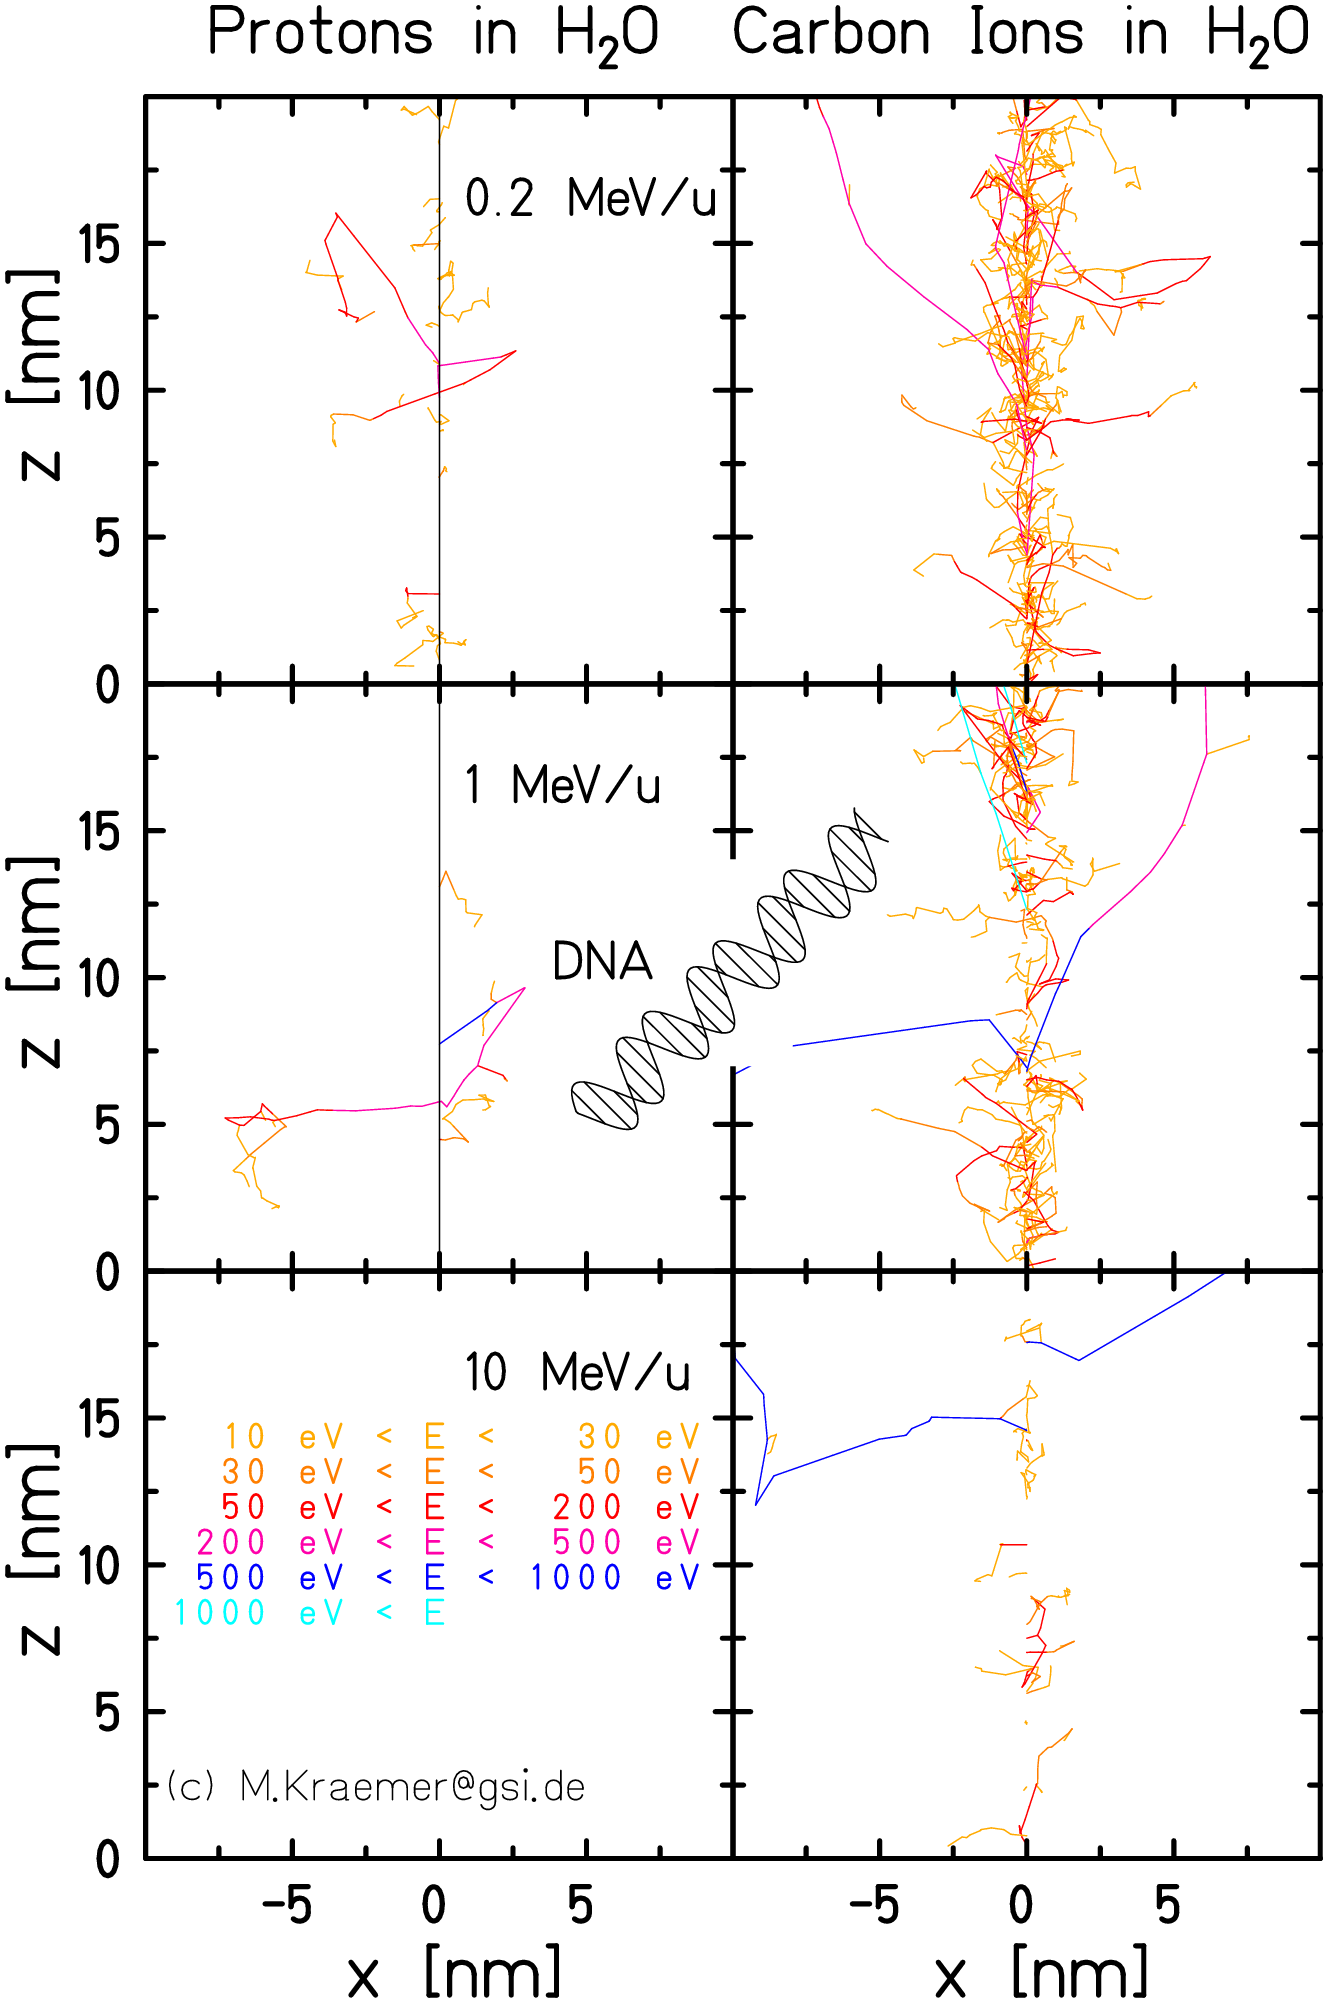
\includegraphics[scale=0.25]{trackstructure.png}
\caption{Microscopic track structure of protons (left side) and carbon ions (right side) at different energies. Protons and high energy 
carbon ions are low LET radiation and hence sparsely ionizing. Low energy carbon ions on the other hand are high LET radiation and hence 
densely ionizing. For comparison the size of the DNA is displayed. Figure courtesy of Michael Kr\"amer.}
\label{track}
\end{center}
\end{figure}



\subsection{Radiobiology}
\label{radiobio}
It was described in the previous section that both, photons and ions, are ionizing radiation producing $\delta$-electrons which 
in turn can cause subsequent ionizations. These ionizations attack the carrier of the genetic information, the DNA, of the irradiated 
cells and hence causes them to stop to proliferate. The biological background of these processes will be described in this section. 
Furthermore the enhanced biological effect of ions compared to photons will be explained. This is one of the potential benefits expected 
from a non-invasive irradiation of atrial fibrillation with carbon ions compared to photons. 


\subsubsection{Impact of radiation on cells}

In eukaryotic cells, meaning cells that contain a cell nucleus, the genetic information is stored in the DNA (deoxyribonucleic acid), 
making it therefore the critical target in radiotherapy. DNA is made of two sugar and phosphate backbones and four different base pairs 
(adenine A, cytosine C, guanine G and thymine T), which bind in a defined way (A with T and C with G) and thus form the double helix 
structure with a distance of the two strands of about 2 nm. The genetic information is encoded in the sequence of the base pairs. 
Ionizing radiation can destroy the described structure of the DNA, either by direct or indirect action \cite{Hal06}.\newline
\newline
As can be seen in figure \ref{ida} direct effects are caused by the destruction of molecular bonds of the DNA itself 
through any form of radiation. This process is considered the dominant effect if radiation with a high energy loss along the particle 
track is used. Indirect action means that free radicals are produced by the ionizing radiation, which then in turn can damage the DNA. 
This phenomenon is predominant when sparsely ionizing radiation (like photons) are used and interact with molecules in the cell, 
particularly water.\newline
\newline
Both mechanisms can cause either single strand breaks (SBS) or double strand breaks (DSB) (see figure \label{ida}). SSB means that only 
one of the strands is destroyed, leaving the complementary base on the other strand intact and thus enabling a fast repair if the SSBs 
occur at a certain distance from each other. DSBs or clustered SSBs are more complex and can cause the breakage of the chromatin. But even 
these damages are usually steadily repaired. The repair mechanisms only start to fail when the DSBs accumulate to local lesions. Changes 
in the original DNA material is the result. Depending on the produced damage mutations, carcinogenesis or cell death can be the 
result. Cell death can occur in different pathways. Apoptosis is the controlled self-inactivation of the cell and the preferred 
pathway in radiotherapy. Uncontrolled cell death, necrosis, typically causes severe reactions of the immune system, leading to e.g. 
inflammation.

\begin{figure}[H]
\begin{center}
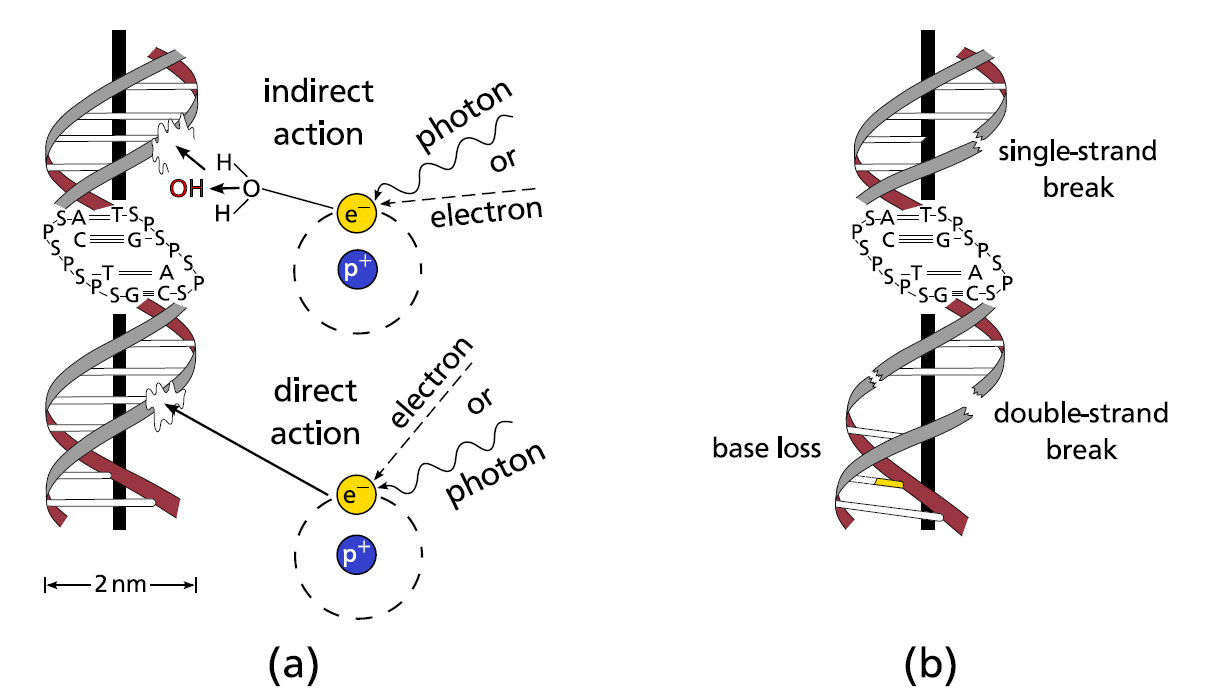
\includegraphics[scale=0.5]{SSB_DSB.png}
\caption{On the left side (a) direct and indirect radiation damages are illustrated. On the right side (b) single strand breaks and 
double strand breaks are visualized. Figure taken from \cite{Ric12}}
\label{ida}
\end{center}
\end{figure}



\subsubsection{Relative Biological Effectiveness RBE}

As outlined, at the same dose level radiation damage depends on the LET.  This means that the induced biological effect 
is, amongst others, dependent on the energy and type of radiation. This is described in the relative biological effectiveness (RBE), 
which is defined as follows:

\begin{equation}
 RBE = \left.\frac{D^{ref}_{photon}}{D_{ion}} \right|_{isoeffect}
\end{equation}

$D^{ref}_{photon}$ is the absorbed photon dose necessary to induce a certain isoeffect and $D_{ion}$ the absorbed dose of ions at a 
defined energy which leads to the same effect. Comparison of RBE values are valid only for the same effect and biological endpoint 
and by using the same reference radiation. This idea is used in the local effect model (LEM) at GSI for the prediction of the RBE. By 
assuming that the biological effect is independent of the specific radiation type but rather on the energy deposition distribution 
in small sub volumes of the cell nucleus, RBE predictions are computed in relation to the known biological response of photons 
\cite{Krae03} \cite{Frie13}. Weighting the physically absorbed dose with the RBE results in the biological dose in units of GyE. \newline
\newline
%% XXX FIGURE RBE
The RBE depends on multiple parameters, like the for example the irradiated tissue and its repair mechanism, the particle type, the used 
dose level and the LET. The dependence between RBE and LET is illustrated in figure \ref{rbe_let}. In case of x-rays (sparsely ionizing) 
the probability of an induced DSB is low and in general more than one track would be required to induce DSBs, resulting in a small RBE. 
Irradiation with a LET around 100 keV/${\mu}$m on the other hand is optimal in producing a biological effect, as the 
density of ionization coincides with the diameter of the DNA double helix of about 2 nm distance. Thus radiation with this LET has the 
highest probability to induce a biological damage with DSBs. More densely ionizing radiation (LET > 200 keV/${\mu}$m) produces many DSBs, 
thereby wasting energy as the ionization events are closer together than needed. The RBE consequently decreases again, an 
effect known as overkill effect. 

% As the RBE is the ratio of doses producing an equal biological effect the RBE value for this radiation type is lower than for the 100 keV/${\mu}$m radiation. 

\begin{figure}[H]
\begin{center}
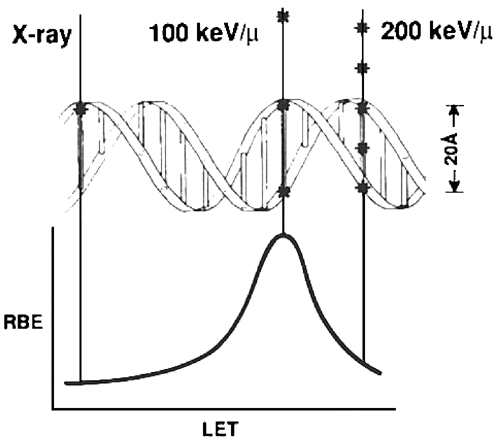
\includegraphics[scale=0.5]{rbe_let.png}
\caption{Radiation with a LET of 100 keV/${\mu}$m has the biggest RBE for cell killing due to the fact that average seperation between 
ionizing events coincides with the diameter of the DNA double helix (2 nm). Figure taken from \cite{Hal06}}
\label{rbe_let}
\end{center}
\end{figure}

Concerning the increased biological effectiveness of ions it can be stated that it is only of advantage if the RBE is more pronounced 
in the target tissue compared to the normal tissue in the entrance channel. While protons exhibit an almost constant RBE throughout the 
energy deposition (a constant value of RBE = 1.1 is used), for ions heavier than oxygen the location for the highest RBE moves towards the 
proximal region of the depth-dose profile, starting to coincide with the plateau region \cite{Kra00}. For carbon ions on the other hand 
the position of the highest RBE value coincides with the Bragg peak region, offering the possibility of a beneficial treatment outcome. 

% In carbon ions, the RBE coincides with the Bragg Peak position \cite{Kra00}, thus enabling to deposit a smaller physical dose in the 
% target and to further reduce the dose to the healthy tissue in the plateau region.  


% \subsubsection{Biological dose}
% \subsubsect<ion{Radiobiological modeling}
% % % - Linear Quadratic model
% % % - LEM
% % % - hohe Dosen


\newpage

%%%%%%%%%%%%%%%%%%%%%%%%%%%%%%%%%%%%%%%%%%%%%%%%%%%%%%%%%%%%%%%%%%%%%%%%%%%%%%%%%%%%

\section{Radiotherapy}

The conventional method for radiotherapy remains the irradiation with photons. Nevertheless, the biological and physical properties of ions 
(which were described in the previous section) result in advantages for radiotherapy, especially when treating deep seated targets. 
As a result, more and more ion facilities are opened worldwide, treating an increasing number of patients with protons and carbon ions. 
In this section the state of the art in treating static tumors with photon and carbon ion therapy will be summarized. 
Afterwards organ motion and the resultant difficulties, as well as approaches for motion mitigation will be presented. 

\subsection{Photon Therapy}

As can be seen in figure \ref{ddp}, a treatment of deep seated targets with photons can be carried out more effectively the higher the photon 
energy. Over the decades, different photon emission techniques were developed which allowed for higher photon energies. 
Currently, photons in the energy range of 6-18 MV \cite{Ber06} are used. The photons are produced with the help of linear accelerators, which 
are used to shoot accelerated electrons on a target, thereby emitting bremsstrahlung which is then used for radiotherapy.\newline
\newline
Like the used photon energy spectrum also the application techniques developed over the last decades \cite{Buc05}. Two dimensional (\textbf{2D}) 
radiotherapy was based on radiographies and was carried out with a single beam, which was applied from one to four different directions, 
usually as opposing lateral fields. As the imaging techniques advanced the treatment became also more conformal. CT scans enabled axial anatomy 
and tumor visualization in three dimensions. Hence in three dimensional conformal radiotherapy (\textbf{3DCRT}) more accurate dose calculations 
with homogeneous fields are possible, leading to an increased healthy tissue sparing. With the development of \textbf{IMRT} (intensity 
modulated radiotherapy) the healthy tissue sparing could be further improved. In IMRT a varying number of beams 
from different beam directions are overlaid, thereby modulating the intensity of radiation within each field. This intensity modulation is 
achieved by using multileaf collimators (MLC) (see figure \ref{lamellen}). An exemplary IMRT treatment plan in comparison to carbon ion 
irradiation can be seen in figure \ref{targetvergleich}. 

\vspace*{-0.3cm}

\begin{figure}[H]
\begin{center}
% 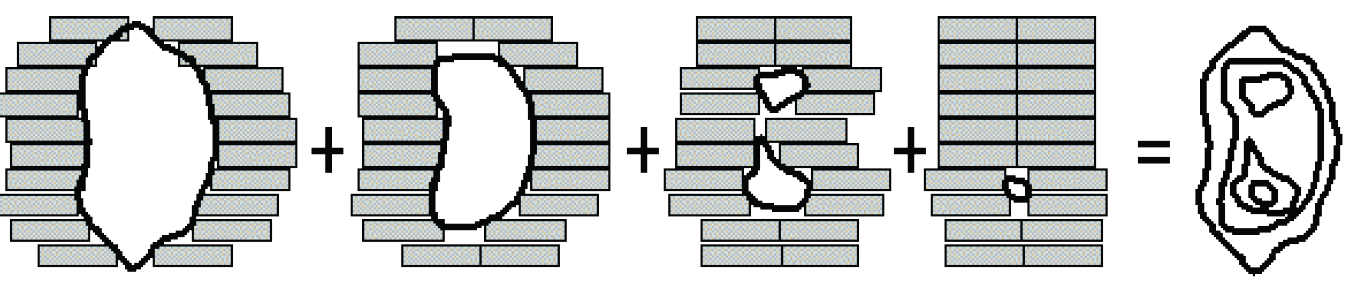
\includegraphics[scale=0.28]{lamellen.png}
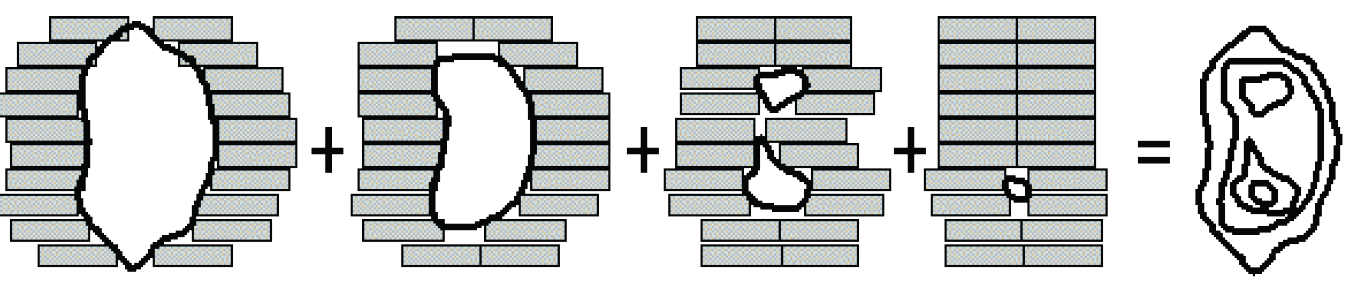
\includegraphics[scale=0.2]{lamellen.png}
\caption{Technical realization of IMRT by the use of multileaf collimators (MLC), enabling a photon dose deposition conformal to the 
target volume. Each lamellae can be moved individually, enabling an intensity modulation. Figure taken from \cite{Schl01}}
\label{lamellen}
\end{center}
\end{figure}

% IMPT is implemented in various ways through different centers, with the most common being the mounting of the 
% photon radiation producing linear accelerator on a gantry \cite{Lue12}. A comparison between conventional 2D radiotherapy with photons 
% and an IMRT treatment can be seen in figure \ref{imrt}. A comparison between IMRT and carbon ion radiation is visible in figure 
% \ref{targetvergleich}.
% 
% \begin{figure}[H]
% \begin{center}
% 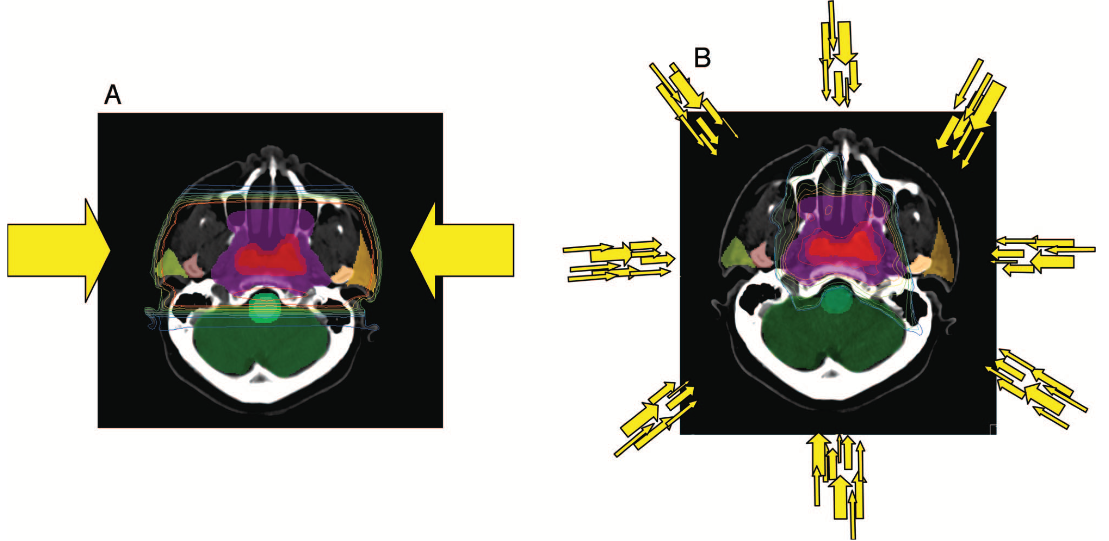
\includegraphics[scale=0.6]{imrt.png}
% \caption{Comparison of dose distributions for 2D photon irradiation with two fields (left side) and IMRT (right side). Superior target 
% conformity and better sparing of normal tissue can be achieved with IMRT. Figure taken from \cite{Buc05}}
% \label{imrt}
% \end{center}
% \end{figure}


\subsection{Carbon Therapy}

As already explained in section \ref{pbb} ions display an inverse depth-dose profile and a higher biological effect compared to photons. 
This enables a high target conformity and a sparing of healthy tissue, both of which are beneficial for radiotherapy. 
% The photon depth dose profile on the other hand limits achievable target conformity for deep seated targets, as advanced as the application 
% methods for photon therapy may be. 
Since 1954, when the first ion beam therapy was carried out with protons at Berkeley Lab \cite{Tob58} different projectile ions were 
used and their effect on target tissue studied.\newline
\newline
Due to the their higher momentum and thus smaller lateral scattering (see section \ref{scat}) the usage of heavy ions (heavier than protons) 
enables a better sparing of healthy tissue and organs at risk (OAR), even if they are close to the target volume. 
In contrast to other ion types, the increased biological effectiveness of carbon ions  coincides with the Bragg peak region (see section 
\ref{radiobio}). Thus both the physical and biological properties of carbon ions offer the possibility of a beneficial treatment outcome. 

\subsubsection*{Application technique}

As in photon therapy, ion therapy application and thus target conformity improved over the decades after first treatments at Berkeley 
were performed by shooting the proton beam through the complete patient head \cite{Tob58}. Depending on the provided accelerator as well 
as on the beam line properties passive and active techniques are distinguished both in beam delivery as well as beam shaping.\newline
\newline
Concerning \textbf{beam delivery} particle acceleration to the therapeutic energies of several hundred MeV/u is carried out in cyclotrons and 
synchrotrons. \textbf{Cyclotrons}, which are used mainly in proton centers, offer the advantage of a more compact design compared to synchrotrons 
and allow a continuous beam extraction with stable intensities. On the other hand no active energy variation is feasible, requiring the need 
for passive energy degraders. \textbf{Synchrotrons}, which are used in heavy ion centers, allow active energy variation.\newline
\newline
Concerning \textbf{beam shaping} methods, which are used in order to deposit a homogenous dose in the target volume, \textbf{passive methods} 
are used in some carbon ion centers as well as in the majority of proton centers. The devices rely on three different beam shaping steps 
\cite{Chu93}. First the beam is broadened by scattering and then further widened by using range modulators like e.g. a 
ridge filter. Thereby an extended and flat, but still homogenous, field is formed which covers the tumor extent in longitudinal direction 
(Spread Out Bragg Peak: SOBP). Secondly, the range adjustment of the SOBP is achieved via flat degraders of variable thickness. Final 
conformity to the distal target border is achieved by patient individual compensators. In the last step, collimators are used for a lateral 
conformity. A scheme of a passive beam shaping system can be seen in figure \ref{passive}. Passive beam shaping devices offer the benefit 
that the historically poor beam quality of research facilities - in which the first treatments were carried out - did not influence the 
homogeneity of the applied dose. Moreover, beam energy changes during treatment can be avoided, thus enabling a fast irradiation time. 
Nevertheless, passive beam application always require the manufacture of patient individual compensators and an unavoidable limitation in 
volume conformity in the proximal tumor region as the SOBP width is fixed by the range modulator to the largest needed depth (see 
figure \ref{passive}). Material in the beam path means furthermore intensity loss due to lateral scattering and an extra dose exposure 
due to fragmentation.

% \begin{figure}[H]
% \begin{center}
% 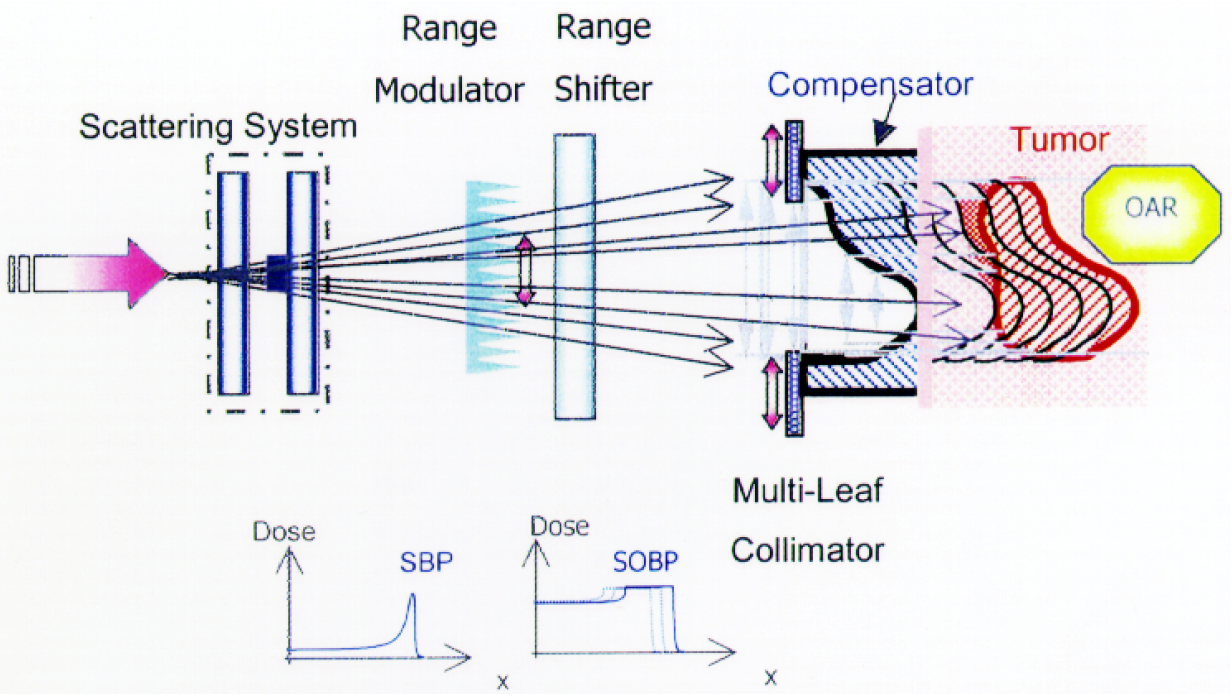
\includegraphics[scale=0.4]{passive.png}
% \caption{Scheme of a passive beam shaping system. Figure taken from \cite{Reg02}}
% \label{passive}
% \end{center}
% \end{figure}

\vspace*{0.8cm}
\begin{figure}[H]
\begin{center}
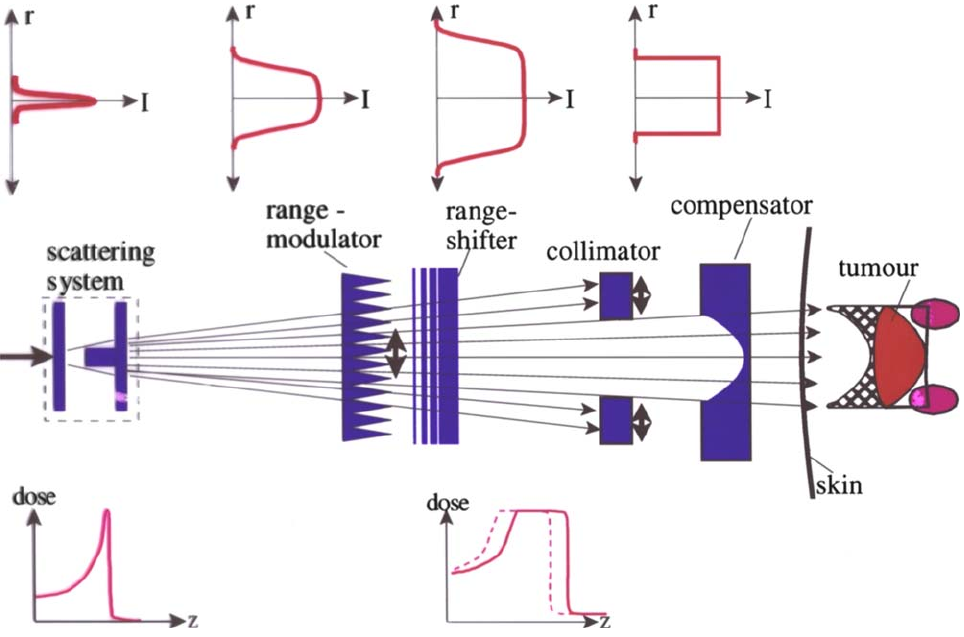
\includegraphics[scale=0.4]{deliverypassive.png}
\caption{Scheme of a passive beam shaping system. The beam is broadened by a scattering system and the width of the SOBP is determined by a 
range modulator. Via a range shifter the SOBP energy can be adjusted to a fixed range and thus depth. For lateral conformity collimators are 
used. The longitudinal conformity to the distal border of the target is achieved with a patient specific compensator. The proximal volume 
border can not be shaped, as is indicated in the hatched areas. Figure taken from \cite{Sch10}}
\label{passive}
\end{center}
\end{figure}

\newpage

\textbf{Active beam shaping} is achieved with beam scanning, which offers a very good lateral target coverage as well as volume conformity 
also in the proximal field region. The target volume is thereby subdivided into slices of the same beam energy, so called iso-energy slices 
(IES). Each IES is again subdivided into a grid of target points which are irradiated sequentially. Hence many small pencil beams are used to 
generate a conform dose deposition to any arbitrary target volume shape without the need of patient specific hardware. This drastically 
decreases the amount of material the beam has to traverse and hence reduces the unwanted neutron dose to the patient \cite{Kad12}. Examples of 
beam scanning are spot scanning, which was developed for protons at the Paul Scherrer Institute (PSI, Swiss) \cite{Ped95} or raster scanning, 
which was developed in parallel at GSI \cite{Hab93}. \newline
\newline
At PSI a cyclotron is used and the energy variation is carried out with a degrader. The lateral deflection of the beam position is either 
achieved with magnets (Gantry 2 at PSI \cite{Ped04}) or a combination of magnets and patient couch motion (Gantry 1). The beam is thereby 
switched off between different beam positions. \newline
\newline
Raster scanning on the other hand works in a continuous mode. A pencil beam is extracted from the synchrotron with a fixed energy and thus range, 
corresponding to a IES of the volume. By overlaying many different energies a SOBP is created to cover the longitudinal extension of the tumor 
(see figure \ref{active}b). The raster points within each IES are irradiated by deflecting the pencil beam via two orthogonal dipol magnets 
on an optimized path. When the pre-defined intensity of the raster point has been reached, the beam is moved to the next position. 
In order to establish a homogeneous dose coverage in the target volume the spacing, both in raster point position as well as IES distance, 
can be utilized. Robustness in longitudinal direction can be achieved with overlap of the individual IES slices. Nevertheless the number of 
IES slices should be kept small in order to guarantee a short treatment time. Hence a broadening of the Bragg Peak position is carried out 
with a so-called ripple filter (see figure \ref{active}b). It was found that a spacing of 3 mm between IESs yields a robust result \cite{Web99}. 
Furthermore the lateral overlap of the pencil beams needs to be chosen in such a way that the possibility of minor fluctuation in beam 
quality and position is compensated for. As the lateral beam profile is assumed to be Gaussian shaped and symmetric it was found that the 
FWHM of the beam is optimally chosen to be three times the raster spacing (see figure \ref{active}a) \cite{Hab93}. 

\newpage

\vspace*{0.6cm}

\begin{figure}[H]
\begin{center}
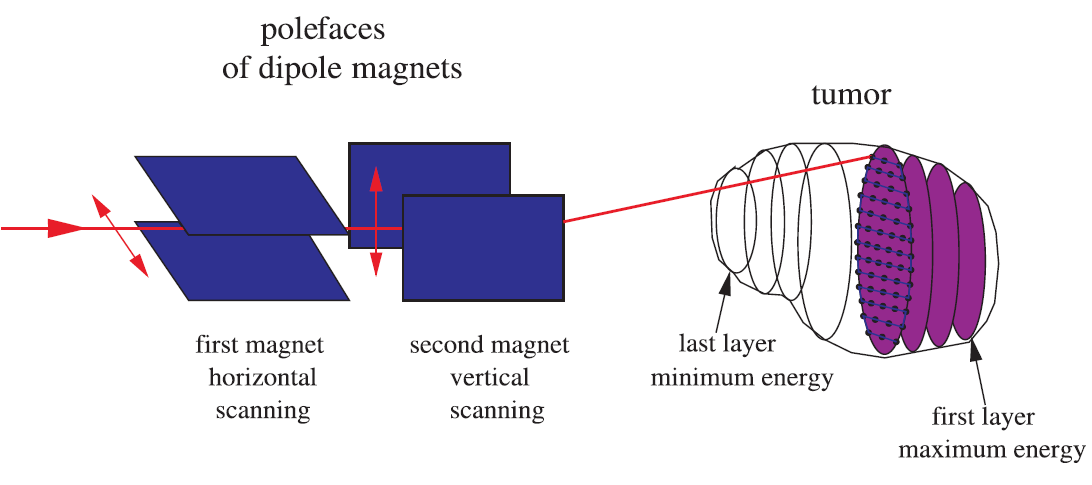
\includegraphics[scale=0.4]{therapy.png}
\caption{Principle of the raster scanning technique at GSI. The target volume is divided into IES, which is again subdivided into a regular 
grid. By varying the particle energy from the accelerator and by deflecting the pencil beam via a magnetic scanning system the raster points 
are scanned. Figure taken from \cite{Inf05}}
\label{scanning}
\end{center}
\end{figure}


\begin{figure}[H]
\begin{center}
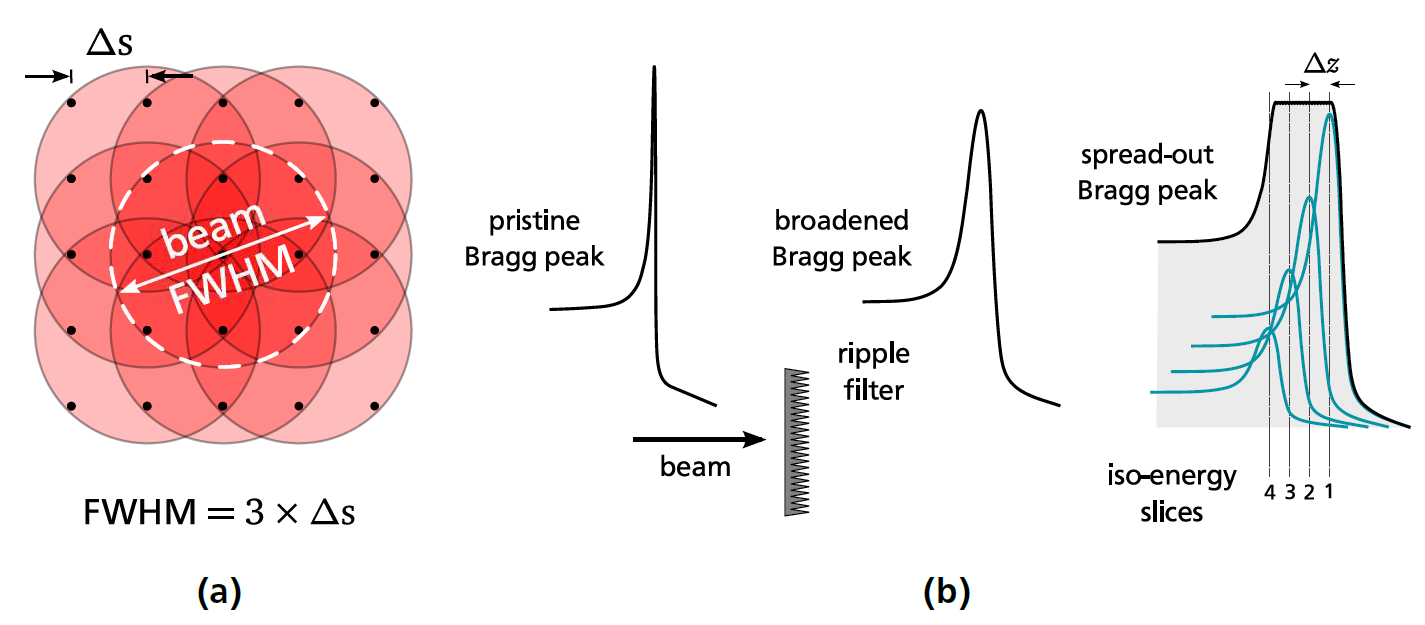
\includegraphics[scale=0.45]{active.png}
\caption{Target dose homogeneity is achieved by sufficient overlap in lateral and longitudinal directio. a) In lateral direction the FWHM of 
the pencil beam is adjusted to three times the raster spacing $\Delta\mathrm{s}$. b) In longitudinal direction the Bragg peaks are broadend 
in depth by using a ripple filter and then stacked in depth to a SOBP. An IES spacing $\Delta\mathrm{z}$ of typically 3 mm is chosen. 
Figure taken from \cite{Ric12}}
\label{active}
\end{center}
\end{figure}


\newpage

\subsubsection*{GSI pilote project}

Between 1997 and 2008 440 patients were treated with scanned carbon ions at GSI. Mostly head and neck tumors were irradiated. 
The typical fractionation scheme was 20 fractions within three weeks \cite{SchE07}. An example of a resulting 
dose distribution with scanned carbon ions in comparison to IMRT can be seen in figure \ref{targetvergleich}. 
The treatment outcome for skull-based chordomas can be seen in figure \ref{chordoma}. In later stage, also prostate and spinal cord 
tumors were treated.

\begin{figure}[H]
\begin{center}
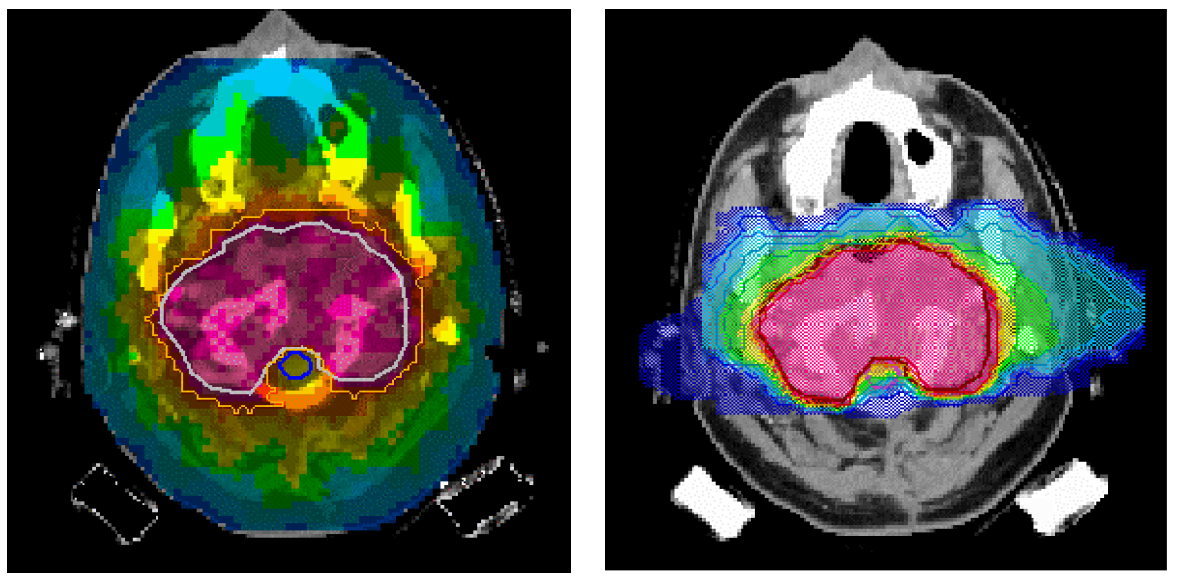
\includegraphics[scale=0.25]{targetvergleich.png}
\caption{Comparison of dose distributions results with IMRT (left side) and scanned carbon ions (right side). The dose to the healthy 
tissue and ecspecially organs at risk like the brainstem are drastically reduced for scanned carbon ions. Figure taken from \cite{Gro04}}
\label{targetvergleich}
\end{center}
\end{figure}

\vspace*{-1cm}

\begin{figure}[H]
\begin{center}
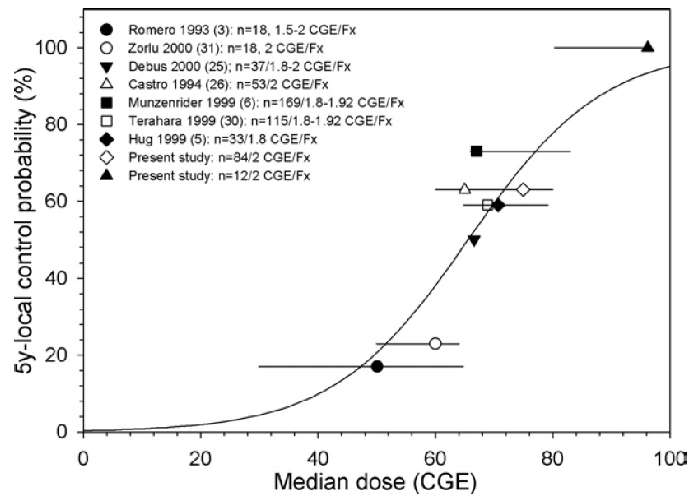
\includegraphics[scale=0.4]{chordoma.png}
\caption{Treatment outcome for the irradiation of skull-based chordomas for photons (left area), protons (middle area) and carbon ions (outer 
right area). An improved effect after the irradiation of chordomas can be seen when doses exceeding 70 CGE can be applied. Due to 
the properties of the scanned carbon ion beam, this dose can be deposited while sparing the nearby OAR. 
Figure taken from \cite{SchE07}}
\label{chordoma}
\end{center}
\end{figure}

The pilot project at GSI was carried out in a collaboration between GSI, the Heidelberg University hospital, the German cancer research 
center (DKFZ) and the research center Dresden-Rossendorf. Based on the success in treatment outcome the Heidelberg Ion-Beam Therapy 
Center (HIT) was build, where patients are treated with scanned carbon ion beams and protons on a regular basis since 2009 \cite{Com10}. 
Furthermore CNAO (centro nazionale di adroterapia oncologica, Pavia, Italy) started treating patients with scanned carbon ions beams 
in 2011 \cite{Ama04}. In total roughly 10,000 patients have been treated with carbon ions up to the beginning of 2013, whereof about 
2,000 patients were treated with scanned carbon ions \cite{PTCOG13}.

% \subsubsection*{Carbon ion centers}

\subsection{Treatment planning}
\label{tp}
Treatment planning is the optimization process in which the needed machine delivery parameters are determined for a chosen beam 
configuration in order to yield the prescribed dose to the target volume, while minimising the dose to the normal tissue, ecspecially 
to the OARs \cite{Ric12}. In modern radiotherapy treatment planning is based on CT scans, which represent photon attenuation through 
the different tissue types (Hounsfield units - HU) and can hence be converted to water-equivalent depths. On the patient image data the 
target and OARs are contured and the needed dose and dose constraints, respectively, are determined. For cancer radiotherapy the delineation 
of the tumor includes certain safety margins, defined by the International Commission on Radiation units and Measurements (ICRU). As some 
of these margins will be also used in the context of cardiac targets, they will be shortly introduced here. 

\begin{enumerate}
 \item [] \textbf{GTV (Gross Tumor Volume)}: "The GTV is the gross palpable or visible/demonstrable extent and location of the malignant 
 growth." \cite{ICRU93a}
 \item [] \textbf{CTV (Clinical Target Volume):} "The CTV is a tissue volume that contains a GTV and/or subclinical microscopic malignant 
 disease, which has to be eliminated. This volume thus has to be treated adequately in order to achieve the aim of therapy: cure or 
 palliation." \cite{ICRU93a}
 \item[] \textbf{PTV (Planning Target Volume):} "The PTV is a geometrical concept, and it is defined to select and appropiate beam size 
 and beam arrangements, taking into consideration the net effect of all the possible geometrical variations, in order to ensure that the 
 prescribed dose is actually absorbed in the CTV." \cite{ICRU93a}
 \item[] \textbf{IM (Internal Margin):} "The IM, commonly asymmetric around the CTV, is intended to compensate for all movements and all 
 variations in site, size and shape of the organs and tissues contained or adjacent to the CTV. They may result e.g. from respiration, 
 different fillings of the bladder, different fillings of the rectum, swallowing, heart beat, movements of the bowel" \cite{ICRU99}
\end{enumerate}

Based on this definition, the \textbf{ITV (Internal Target Volume)} is commonly used for the volume in which the IM encompasses the CTV. 

\begin{figure}[H]
\begin{center}
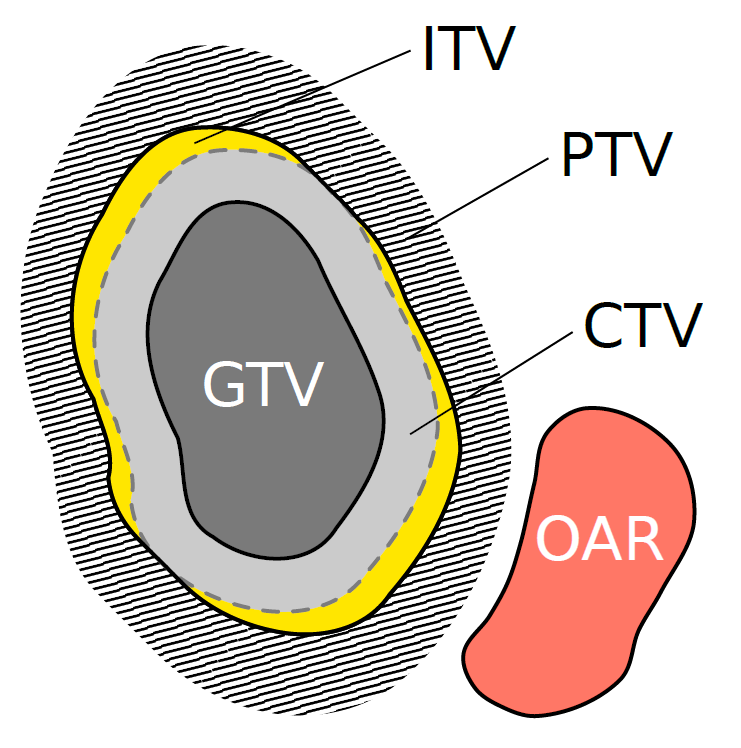
\includegraphics[scale=0.3]{volumes.png}
\caption{Treatment planning volumes as defined by the ICRU. Figure taken from \cite{Ric12}}
\end{center}
\end{figure}

\vspace*{-0.3cm}

% After delineation, the number of fields as well as the field angles are chosen in such a way that the OAR are spared as good as possible. 
As a result of treatment planning the ICRU recommands that 100\% of the PTV should receive at least 95\% and not more than 107\% of the 
prescribed dose \cite{ICRU93a}. In order to study if this recommandations are met, dose-volume-histograms (DVH) are computed in the 
treatment planning study process and the values V95 and V107 (the volume which receives 95\% and 107\% of the dose, respectively) determined. 
Furthermore D5 and D95, which denotes the dose covering 5\% and 95\% of the volume, are extracted. The difference between these two values 
(D5-D95) is a measure for the dose fall off and should be ideally close to zero. In general, the dose constraints of the OAR depends on the 
organ as well as fractionation scheme and radiation type and needs to be carefully examined in each individual case.\newline
\newline
The treatment planning system and hence its result, the dose optimization, depends on the radiation type and on the used beam delivery 
technique. For scanned carbon ion beams the optimization task with the in-house treatment planning software TRiP98 \cite{Krae00} 
\cite{Krae00b} needs to determine the required energies of the IESs and the pencil beam positions as well as corresponding particle numbers 
for each raster point. This leads to an 'inverse' optimization process, in which the particle fluence to the target volume, which is given in 
the form of planar polygon originating from manual delineation on the axial CT slices \cite{Ric13}, is determined from the prescribed dose 
distribution \cite{Kra00}. Furthermore, as the irradiation is 
carried out starting from the most distal IES a certain dose is already deposited in the more proximal slices. Thus only the distal slice 
receives a homogeneous fluence distribution while all other slices require irregular dose patterns (see figure \ref{inhomo}). Using the 
physical and biological beam models (LEM, see RBE in section \ref{radiobio}) the dose contributions from all raster points to each 
individual target voxel are calculated \cite{Ric12}. 

% In order to achieve this the ion specific properties as well as the capabilities of the GSI scanning system have to be 
% taken into consideration.

\begin{figure}[H]
\begin{center}
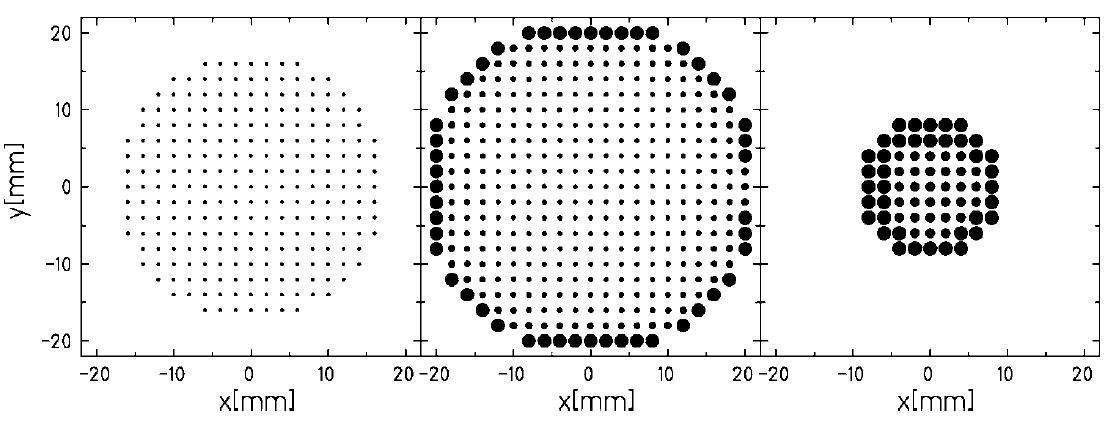
\includegraphics[scale=0.4]{inhomo.png}
\caption{Particle fluence distribution depending on the IES, starting with the most distal one (left) and moving to more proximal regions. 
Figure taken from \cite{Krae00}}
\label{inhomo}
\end{center}
\end{figure}

% \vspace*{-1cm}

\subsection{Organ motion in radiotherapy}

Many target sites are influenced by temporal changes. Depending on the underlying mechanism, one distinguishes patient positioning 
related organ motion and organ motion in-between treatment fractions (interfractional motion) or during a treatment 
application (intrafractional motion). The different organ motion types will be specified in this section. Furthermore motion acquisition 
strategies as well as techniques to overcome the motion influence, so called motion mitigation techniques, will be presented. Finally an 
overview over the treatment planning workflow including motion (four dimensional - 4D) will be given. 

\subsubsection{Motion types}

An overview of the different organ motion types is given by Langen and Jones \cite{Lan01}. Three main categories can be determined: 
patient positioning related motion, interfractional motion and intrafractional motion. Examples of these different motion types can be seen 
in figure \ref{motion}. It should be noted that all motion types can occur in a patient. Thus when dealing with intrafractional motion, 
interfractional motion as well as patient positioning needs to be accounted for.\newline
\newline
\textbf{Patient positioning} can cause changes in tumor shape as well as uncertainties in the tumor position. A difference in positioning 
between image acquisition (e.g. CT) and treatment delivery may introduce systematic displacements and hence threaten the outcome of the 
treatment. Patient fixation systems and dedicated protocols are applied to overcome this motion influence. Stereotactic fixation with e.g. 
masks are used on a daily basis. The other two motion types however are purely internal and are distinguished occurring to the time scale 
they occur on.\newline
% \newline
\newpage
\textbf{Interfractional motion} occurs within hours and days, hence between two treatment sessions (if multiple fractions 
are applied). Anatomical changes caused by interfractional motion are manifold. Prostate cancer patients are often subject to position 
changes due to varying gut and bladder fillings \cite{Fok04}. For lung cancer patients, changes in the breathing pattern are troublesome. 
Sonke et al. \cite{Son08} reported that even though the respiratory motion trajectory is often reproducible, the baseline of the tumor 
motion can vary significantly. Cancer patients in general are also subject of tumor shrinkage \cite{Mor09}. In order to mitigate 
interfractional motion, repeated imaging needs to be carried out.\newline
% (adaptation of dose delivery: adaptive radiotherapy ART) \cite{Son10} \cite{Mur11}.
\newline
\textbf{Intrafractional motion} occurs on a time scale of seconds to minutes. The main reason for intrafractional motion are respiration 
and heart beat. Even though the exact motion patterns varies from patient to patient, it can be stated that breathing is a quite regular 
and slow process, with a rather big amplitude. Heart beat on the other hand has a smaller amplitude compared to respiration, but it is a 
high frequency motion with 60 to 80 heart beats per minute compared to 10 to 15 respiration cycles in the same time. These two motions 
superimpose and the influence of both will be studied in the framework of this work when targeting sites in the heart. Different motion 
mitigation techniques for intrafractional motion will be presented in a seperate subsection. 

\begin{figure}[H]
\begin{center}
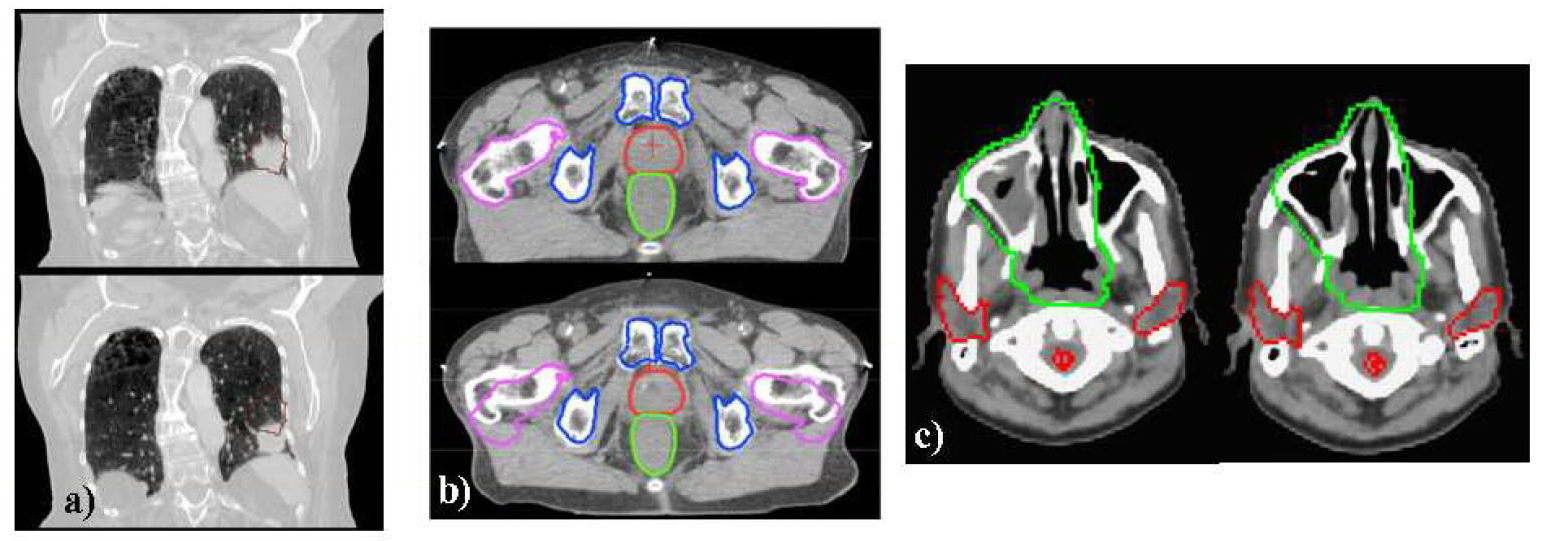
\includegraphics[scale=0.43]{motion_examples.png}
\caption{Examples of the three major motion categories. On the left side (a) a lung tumor is displayed, which moves due to the respiration 
of the patient (intrafractional motion). Interfractional position changes are examplary shown in the middle (b), where two CT scans of a 
prostate patient are compared. Density variations between two CT scans are shown in (c). Figure taken from \cite{Eng11}}
\label{motion}
\end{center}
\end{figure}

\subsubsection{Motion acquisition}
\label{Motionacq}
For a successful irradiation of the moving target, the intrafractional motion of the target site must be known during the treatment process. 
This is for example achieved by time resolved computed tomography scans (4D-CTs) and the potential usage of online motion measurement.\newline
\newline
For the aquisition of 4D-CT scans the motion signal is recorded during the imaging. The motion cycle is then divded into $N$ quasi-stationary 
sections (so-called motion phases (MP)). In every MP a full regular CT scan is reconstructed. In order to achieve this data is recorded in every 
slice for a whole motion cycle. By correlating the data information gained from the motion signal with the recorded CT information, the 
scans are afterwards rearranged according to their affiliation to a certain MP. For more information on 4D-CTs the reader is refered to 
e.g. \cite{Rie05}.\newline
\newline
For 4D-CT image sorting as well as for the application of motion mitigation techniques (see subsection "motion mitigation techniques"), 
the intrafractional motion of the patients needs to be measured. A review of the different techniques can be found at \cite{Eva08}. 
One distinguishes between direct measurement techniques and surrogate signals. Examples for direct measurements are ultrasound and 
fluoroscopy. In fluoroscopy, the patient is irradiated with X-rays and the absorption pattern is displayed on a fluorescent screen, hence 
limiting the acquisition time of this method by the deposited dose. The monitoring time in ultrasound is not limited since no ionizing radiation 
is needed and hence a real time imaging is feasible \cite{Pra12}. Nevertheless influence of air limits the resolution and thus raises 
difficulties when being applied in the thorax region of the patient. Surrogate signals detect variables which are directly related to the 
source of organ motion. Examples of these kind of techniques for respiration are methods which correlate the movement of the torso to the 
phase in the respiration cycle. This can be achieved for example by monitoring the height of the patient surface with camera systems or laser 
displacement sensors and the possiblity for additional infrared markers attached to the patient's body \cite{Tad98} \cite{Ber05} \cite{Schw04}. 
Alternatively the volume of the torso can be measured by using a belt-like strain gauge \cite{Li06}. Other approaches measure e.g. the airflow 
of the patient \cite{Kub96} \cite{Han99}.\newline
\newline
Combinations between direct measurement techniques and surrogate signal acquisition exist and are e.g. used in the 
Cyberknife system. Their Synchrony system (see also \ref{cardiacradiosurgery}) combines fluoroscopy (direct) with an infrared camera 
system (surrogate). This offers the advantage of a drastically reduced fluoroscopy acquisition time as it is only used to check and 
update the surrogate system \cite{Sha10} \cite{Lue12}.

\newpage

\subsubsection{Motion mitigation techniques for intrafractional motion}

% In conventional radiotherapy and passive particle therapy, moving targets are treated by enlarging the safety margins to the target region 
% (irradiating the ITV, which encompasses the target motion - see sections before). A homogenous dose distribution is thereby achieved. 
% In treatment modalities like IMRT and 
In particle beam scanning the beam delivery interferes with the intrafractional target 
motion, causing local over- and underdosages in the target volume, an effect known as Interplay \cite{Phi92} \cite{Ber08}. 
The exactly resulting interplay pattern is dependend on many different factors, like the beam direction, the scanning speed, the motion 
amplitude and starting phase etc. Hence it can not be avoided or directly compensated. Thus techniques which mitigate the influence 
of the underlying target motion have to be applied. The three main techniques (rescanning, gating and tracking) will be explained in more 
detail.\newline
\newline
\textbf{Rescanning}, also known as repainting, is a specific approach for beam scanning and based on statistical averaging of different 
interplay patterns \cite{Phi92} \cite{Rie10}. Scanning the target $N$ times with a reduced dose of $\mathrm{1}/\mathrm{N}$ results in a 
Gaussian distributed dose around the theoretically intended one (see figure \ref{rescanning}). As the variance of the distribution is proportional 
to $\mathrm{1}/\mathrm{\sqrt{N}}$ the result will be better the more rescans are used. The technical realisation of rescanning is easier than 
for e.g. gating and beam tracking, 
ecspecially as it does not require real-time motion monitoring, and results in a homogenous dose to the inner region of the target when 
using enough rescans $N$. Anyhow it can lead to an increased dose deposition to the surrounding, healthy tissue and to under dosages in 
the outer part of the target volume. So far rescanning has not been used in patient treatments, but certain centers (e.g. NIRS \cite{Fur07}) 
and PSI \cite{Zen10}) plan it for the future.

\vspace*{-0.4cm}

\begin{figure}[H]
\begin{center}
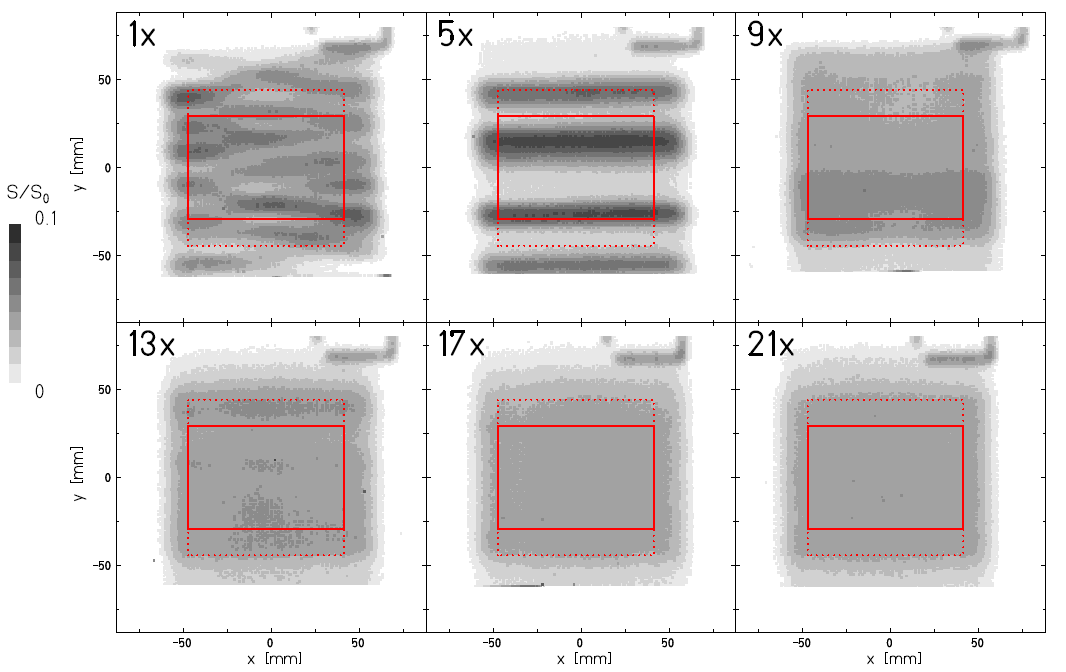
\includegraphics[scale=0.45]{rescanning.png}
\caption{Principle of rescanning in film irradiations. Averaging multiple interplay patterns leads to a homogeneous dose in the target area 
(solid red square). Figure taken from \cite{Ber09b}. }
\label{rescanning}
\end{center}
\end{figure}

\textbf{Gating} is the interrupted irradiation of the target during a selected part of the motion cycle, the gating window \cite{Min00} 
\cite{Li06} (see figure \ref{gating}). Typically a gating window around the most reproducible motion states are chosen, which show a comparable 
small motion (e.g. end exhale in case of respiration). This technique is also used for passive beam delivery, as it reduces the size 
of ITV margins. In the gating window a small motion, the so-called residual motion, remains. In case of beam scanning this can result in 
small interplay effects. Different approaches are studied to overcome this drawback \cite{Fur07} \cite{Zen10} \cite{Ber09}. Gating requires 
online motion monitoring and prolongs the treatment time. For centers with passive beam delivery gating has already been successfully 
used \cite{Min00} \cite{Iwa10} \cite{Has06}.

% \vspace*{-0.6cm}

\begin{figure}[H]
\begin{center}
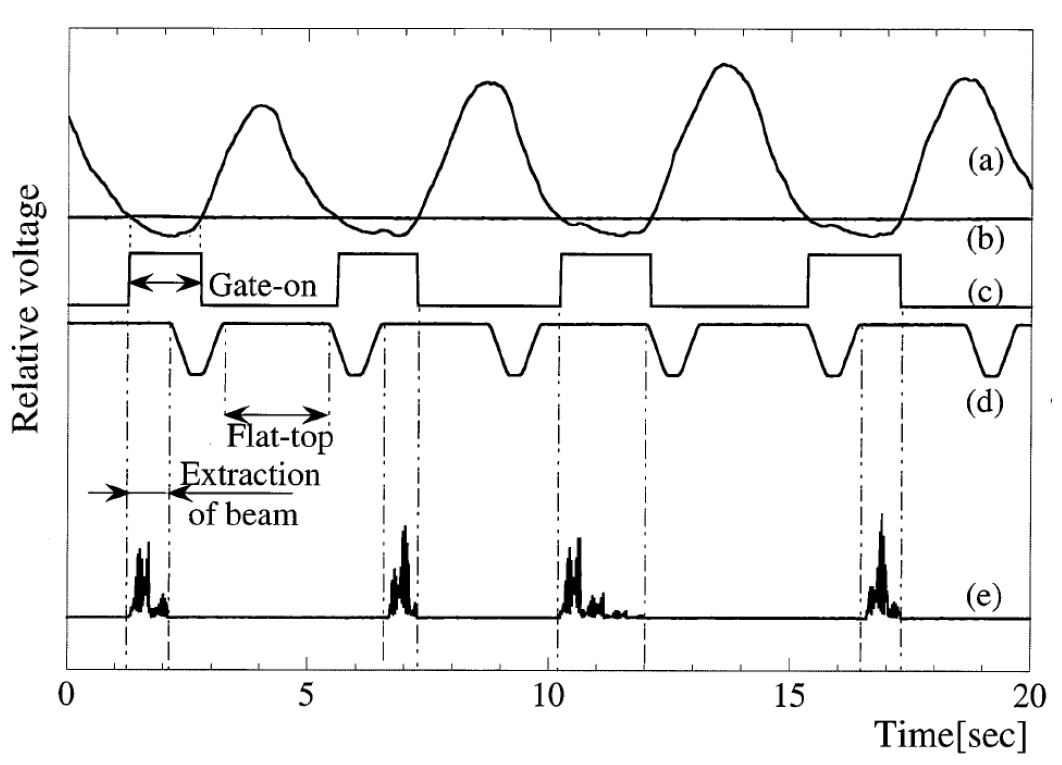
\includegraphics[scale=0.45]{gating.png}
\caption{Principle of gating. Line (a) is the respiratory signal. At end exhale the gradient of the respiration is flat, enabling an 
irradition without large effects of the target motion. The beam (c) is thus only applied during this time. The gating window is activated 
as soon as the respiratory motion crosses line (b). Figure taken from \cite{Min00}}
\label{gating}
\end{center}
\end{figure}


\textbf{Beam tracking} of organ motion requires the adaptation of the beam position to the target motion in real time. It was originally proposed 
for IMPT \cite{Kae01} and ideally requires no additional margins, nor prolongs the treatment time. Prerequisite of this medthod is a fast beam 
delivery system. Tracking is clinically used in the Cyberknife Synchrony system (see section \ref{cardiacradiosurgery}). 
In comparison to photon irradiation, tracking with particles needs a careful consideration and adaptation of longitudinal changes due to 
the Bragg Peak structure of ions. The implemented tracking system at GSI \cite{Gro04} uses fast deflecting dipole magnets, which 
are also used for beam scanning, for the lateral adaptation of the beam. The longitudinal changes are accounted for by two polymethyl 
methacrylate (PMMA) wedges, which are mounted on a fast, linear stepmotor close to the target (see figure \ref{tracking}) \cite{Sai09}. By 
changing the relative distance between the wedges, the beam penetrates PMMA with different energies, thereby changing its energy and 
hence position. Even though the high precision of the system has been proven \cite{Ber07} \cite{Ber10} \cite{Sai09} a clinical use 
is not feasible yet due to the lack of fast and precise real-time internal motion monitoring that includes particel range information.

\begin{figure}[H]
\begin{center}
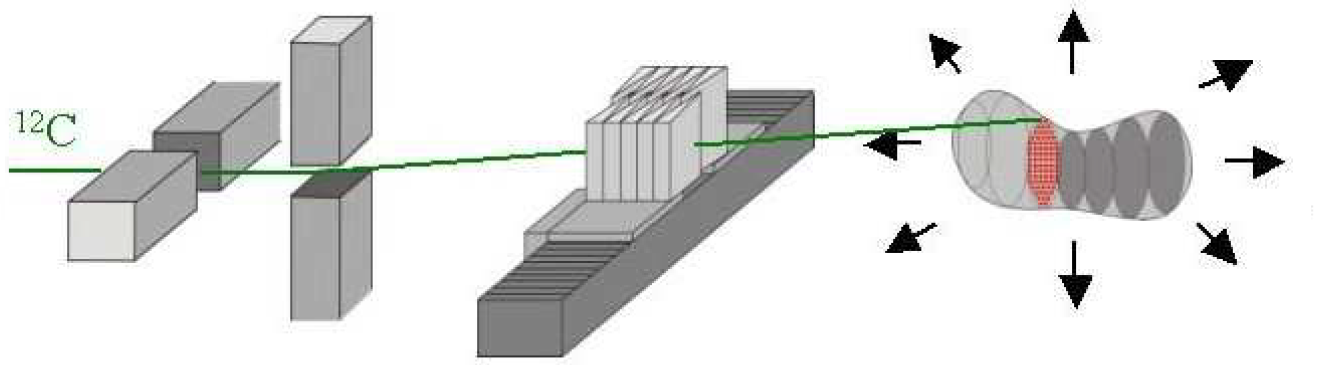
\includegraphics[scale=0.4]{tracking.png}
\caption{Principle of tracking at GSI. The lateral deflection is achieved via dipole scanner magnets. For the longitudinal adaptation two 
PMMA wedges are mounted on step motors, enabling to change the depth the particle beam has to traverse. Figure taken from \cite{Gro04}}
\label{tracking}
\end{center}
\end{figure}

Besides these major motion mitigation techniques, different combinations are currently studied. A combination between rescanning and 
gating is e.g. studied by Furukawa et al. \cite{Fur07} and a combination between rescanning at tracking by van de Water et al. \cite{Wat09}.\newline
\newline
As breathing is the main reason for intrafractional motion in most radiotherapy applications, many different other techniques have been 
investigated to directly mitigate the influence of respiration. An example is abdominal pressure, which has been used in lung 
and liver cancer patients in treatments with photons \cite{Neg01} \cite{Hof03} and recently also for scanned carbon ions at HIT (treatment 
of hepatocellular cancer \cite{Com11}). Jet ventilation \cite{Hof03} and apneic oxygenation \cite{RPTC12} are also used to partially or 
completely suppress respiration of the patient. 


\subsubsection{4D Treatment planning at GSI}

In order to account for intrafractional organ motion, time-resolved (4D) treatment planning is needed. The underlying data as well 
as the techniques for 4D treatment planning will be presented for the special case of scanned carbon ion beams at GSI.\newline
\newline
As in the static case, treatment planning for ions is based on CT scans. In the special case of 4D treatment planning, these CT scans are 
time resolved (\textbf{4DCT}s, see section \ref{Motionacq}, Motion acquisition). In order to use the information stored in the 4DCT, an \textbf{image 
registration} needs to be performed. With this a voxel-to-voxel mapping between the reference phase of the 4DCT and all other motion phases is 
gained, hence yielding a spatial correlation between the individual CT phases \cite{Ric13}. Usually, rigid and deformable registration 
methods are distinguished. While rigid registration only contains linear transformation of the original object in all three room dimensions, 
deformable registration also accounts for compression. Registration is based on registration algorithms, whereof different approaches 
exist. Brock et al. \cite{Bro10} published a multi-institutional study where the accuracy of some of the available algorithms is 
presented. It can be stated that registration accuracy of most algorithms is in the order of millimeters, hence in the order of a CT 
voxel size, but is dependent on the image contrast (resulting in less accurate results when the contrast is diminished).

\begin{figure}[H]
\begin{center}
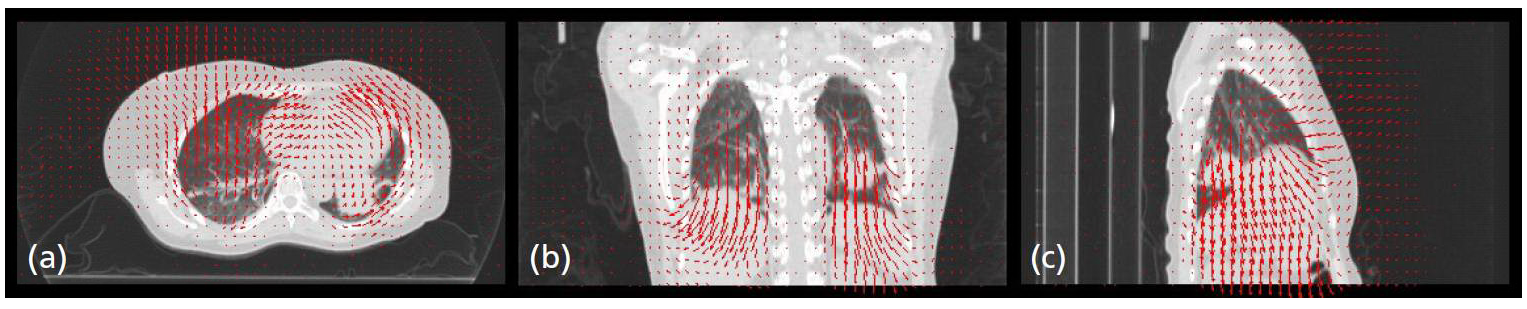
\includegraphics[scale=0.43]{registration.png}
\caption{End-exhale, 4D reference phase of a lung cancer patient with overlying deformation field to end-inhale in a) axial, b) coronal and 
c) sagittal view. Figure taken from \cite{Ric12}.}
\end{center}
\end{figure}

\vspace*{-0.8cm}

\textbf{4D treatment planning} at GSI is carried out with the in-house software \textbf{TRiP4D}. It was mainly developed by Daniel Richter \cite{Ric13} and 
is based on TRiP98 as well as a predecessor program developed by Bert and Rietzel \cite{Ber07b} together with the biological implementation 
under influence of target motion by Gemmel et al. \cite{Gem11}.  
TRiP98 was developed for static target regions and was successfully applied in the GSI pilot project \cite{Krae10} \cite{Krae00} \cite{Krae00b}.  
It is a command-line-based software without graphical interface which runs on an IBM AIX operating system and is written in C 
programming, using a pseudo object-oriented structure. For a detailed description of TRiP4D functionalities as well as the software 
design and experimental verification the reader shall be referred to \cite{Ric13}. A short overview of some of the most important 
functionalities will be given.\newline
\newline
The \textbf{4DCT structure} was implemented as a sequence of 3DCTs with a distinguished reference CT on which the dose optimization 
process is carried out. Thus the existing 3D functionalities, like the computation of water-equivalent path lengths, could be reused. 
Individual phases of the 4DCT are indexed by their position in the motion cycle. 
TRiP4D does not include native \textbf{image registration} functionalities but rather integrates and processes image registration output, obtained e.g. 
with the open source software package Plastimatch \cite{Sha07}. The resulting deformation maps need to be obtained in two directions 
(reference-moving and moving-reference) as certain steps of the treatment planning like contour propagation require the inverse deformation 
maps.
\textbf{Contours segmentation}, of target volumes as well as organs at risk, is stored as a volume dataset model, based on the 3D 
segmentation module of TRiP98 with planar polygons on axial CT slices. Based on this 4D segmentation functionality ITVs (see section \ref{tp}) 
can be created, which are needed for certain motion mitigation 
techniques like e.g. rescanning. In general, the 4D treatment plan generation and \textbf{dose optimization} is very dependent on 
the employed motion mitigation technique. For the ITV concept \cite{Gra12}, and hence in motion mitigation techniques where the dosimetric 
effects caused by interplay are compensated but not the target motion itself, dose optimization is carried out on the 4DCT 
reference phase \cite{Ric13}. For beam tracking on the other hand additional optimization is carried out, as motion compensator vectors have 
to be computed. Furthermore 4D optimization techniques (which include the target motion for optimization by using the full 4DCT dataset, the 
vectors from image registration as well as 4DVOIs for dose optimization \cite{Gra13} \cite{Ele12}) can be developed and applied with TRiP4D.   
Based on the predecessor program by Bert and Rietzel the \textbf{treatment plan} is then split into quasi-static sub-plans 
where the raster points and the corresponding intensities are divided according to the motion phase they shall be irradiated in. 
For the overall \textbf{4D dose calculation} in TRiP4D, the sub-plans are then collected over all motion states for each dose voxel. Thereby 
the voxel position is transformed according to the deformation maps and by accounting for the radiological density distribution of 
the respective phase of the 4DCT. The total physical dose results as a summation of the dose distribution from all motion states in 
the reference state (see figure \ref{TRiP4Ddose}).  For the biological dose calculation the particle and energy spectra are also accumulated 
over all motion states and used as an input for LEM to calculate the RBE. TRiP4D was extensively tested and verified in numerous experiments 
\cite{Ric12} \cite{Ric13}.  


\begin{figure}[H]
\begin{center}
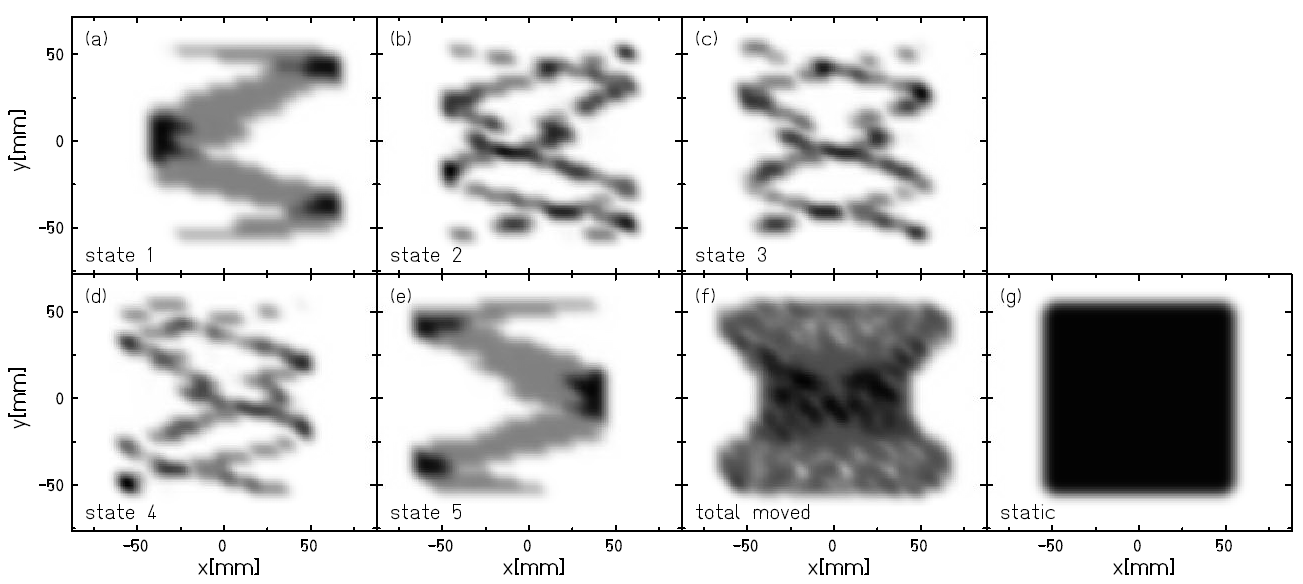
\includegraphics[scale=0.4]{4DtreatmentPlanning.png}
\caption{4D dose calculation with TRiP4D and the resulting film response in experimental validation. Images a)-e) show the individual dose 
deposition in each of the five motion states. In f) the total dose deposition in 4D is displayed. On the stationary film in g) a homogeneous 
dose is deposited in 3D. Figure taken from \cite{Ric12}.}
\label{TRiP4Ddose}
\end{center}
\end{figure}



\newpage

%%%%%%%%%%%%%%%%%%%%%%%%%%%%%%%%%%%%%%%%%%%%%%%%%%%%%%%%%%%%%%%%%%%%%%%%%%%%%%%%%%%%
\section{Atrial fibrillation}

Atrial fibrillation (AF) is the most common cardiac arrhythmia. It occurs in $\sim$2 \% of the general population leading to over six million 
patients in Europe \cite{ESC10} and over two million patients in the United States \cite{CE09}. The lifetime risk of developing AF is 
$\sim$ 25\% in people over forty. Since age is an important risk factor for this cardiac arrhythmia the prevalence is estimated to double in 
the next fifty years due to ageing of society (see figure \ref{USincidences}).\newline

\begin{figure}[H]
\begin{center}
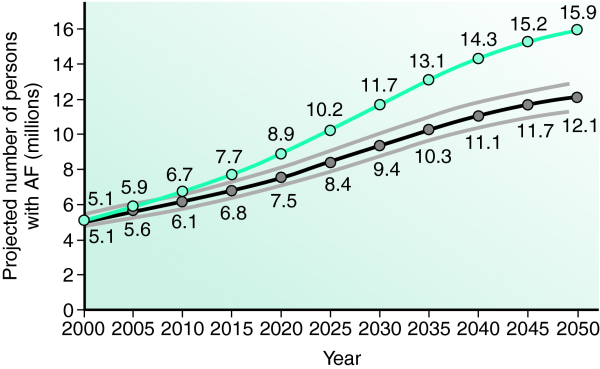
\includegraphics[scale=3]{af_incidences_us.png}
\caption{Trend of AF incidences. The black curve indicates the projected number of patients assuming no further increase in age-adjusted AF 
incidences. The green curve represents the trend assuming a continuous increase in incident rates as evident in 1980 to 2000. Figure taken 
from \cite{Miy06}}
\label{USincidences}
\end{center}
\end{figure}

Even though not in itself life threatening, it dramatically alters the quality of life and increases the risk to suffer a stroke. It is 
estimated that the stroke risk in AF patients is 5-fold higher \cite{Ben98} \cite{Wol91}. AF often remains undiagnosed 
(silent AF). It is stated that one out of five acute strokes is attributed to AF \cite{ESC10}. Other late effects and related events 
include cognitive dysfunctions like vascular dementia and impairment of left ventricular function. In general death rates are stated to 
approximately double by AF \cite{ESC10}, leading to a ten year survival rate of 25 \% compared to 46 \% in patients with a normal sinus 
rhythm \cite{ACC06}.\newline
\newline
In the following the normal signal propagation through the heart's conduction system will be explained in order to contrast the occurring 
differences in AF. Possible causes for AF and underlying risk factors as well as current treatment modalities will be presented.

\newpage

\subsection{Heart's conduction system}

The conduction system of the heart controls the generation and propagation of electrical signals, so called action potentials, that cause 
the heart muscle to contract and hence to pump blood \cite{Med}. The small electrical activity of the action potentials is measurable at the 
surface of the body, enabling a graphical record with an electronic recording instrument, the Electrocardiograph (ECG). In the following the 
events during a single heart beat and the corresponding detection in an ECG (see fig. \ref{ecg}) will be explained. 
The action potentials can originate spontaneously in any of the specialized cardiac muscle cells which form the conduction system. In a healthy 
heart each beat begins in the right atrium with an action potential from the sinoatrial (SA) node (see fig. \ref{condsys}), making it the 
natural pacemaker of the heart. The signal then spreads across both atrial chambers causing the muscle cells to contract (atrial systole) 
which is represented as the P-wave in an. It is followed by a period of conduction (PR-segment in ECG) in which the signal enters the 
ventricles via the atrioventricular (AV) node. As the signal spreads the ventricles contract very rapidly 
(ventricular systole), which is displayed in the QRS-complex in an ECG. Atrial activity is hidden in the ECG by the QRS complex. As the signal 
passes out of the ventricles, the ventricular walls start to relax (ventricular diastole). The T-wave marks this ventricular repolarization. 
The sequence of these events and the corresponding ECG traces repeat with every single heartbeat.\newline

% \vspace{-7cm}
% \vspace{-1.5cm}
\vspace{-0.5cm}
\begin{figure}[H]
\begin{center}
% 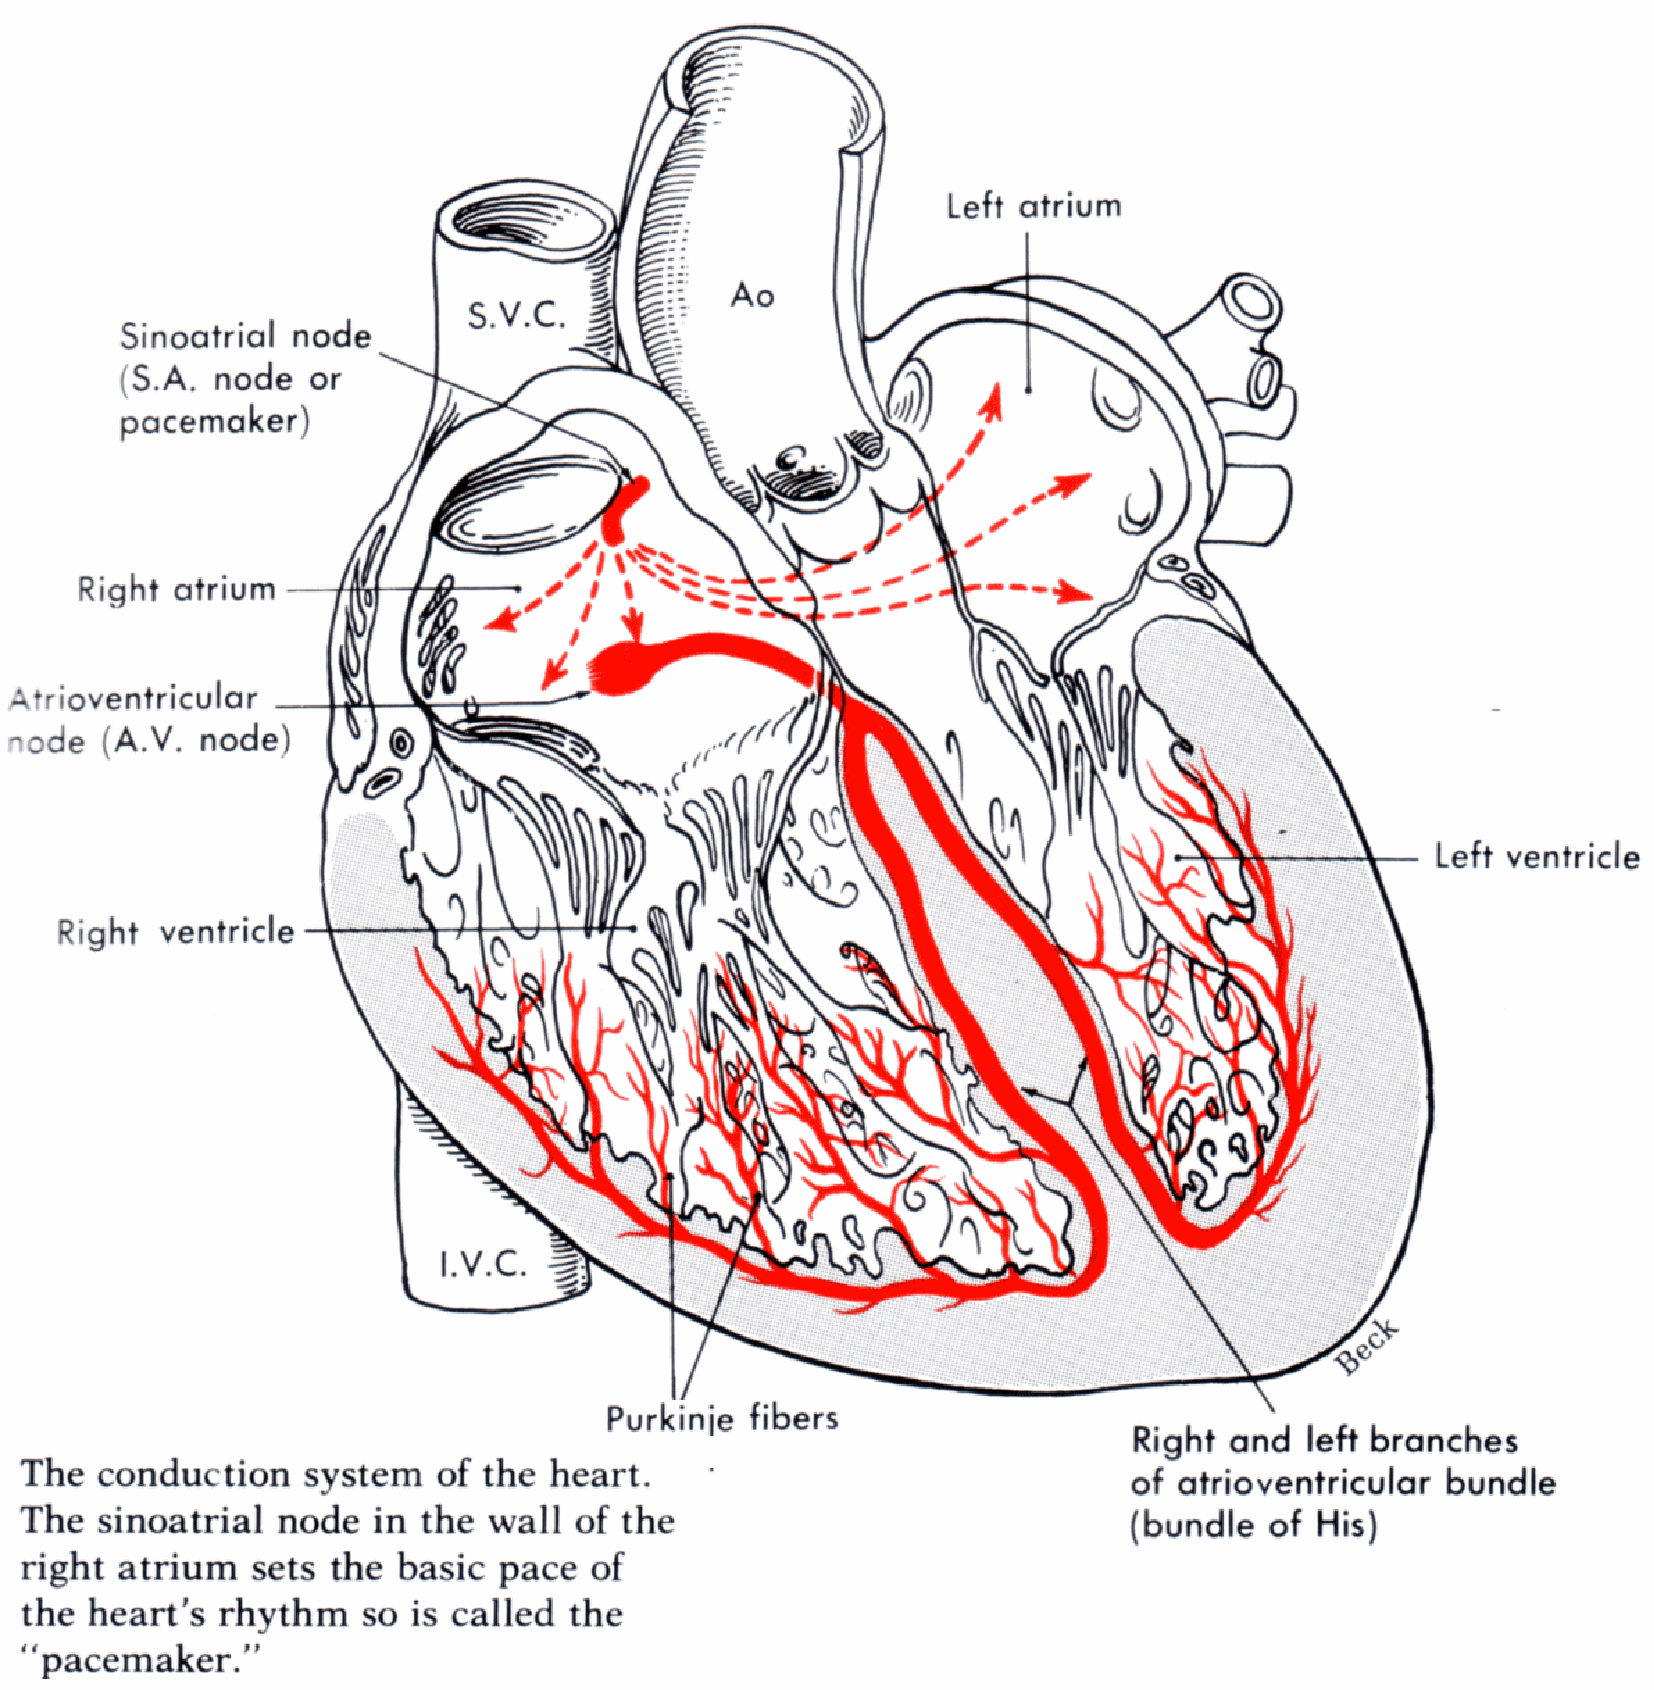
\includegraphics[scale=0.3]{conduction_system.png}
% 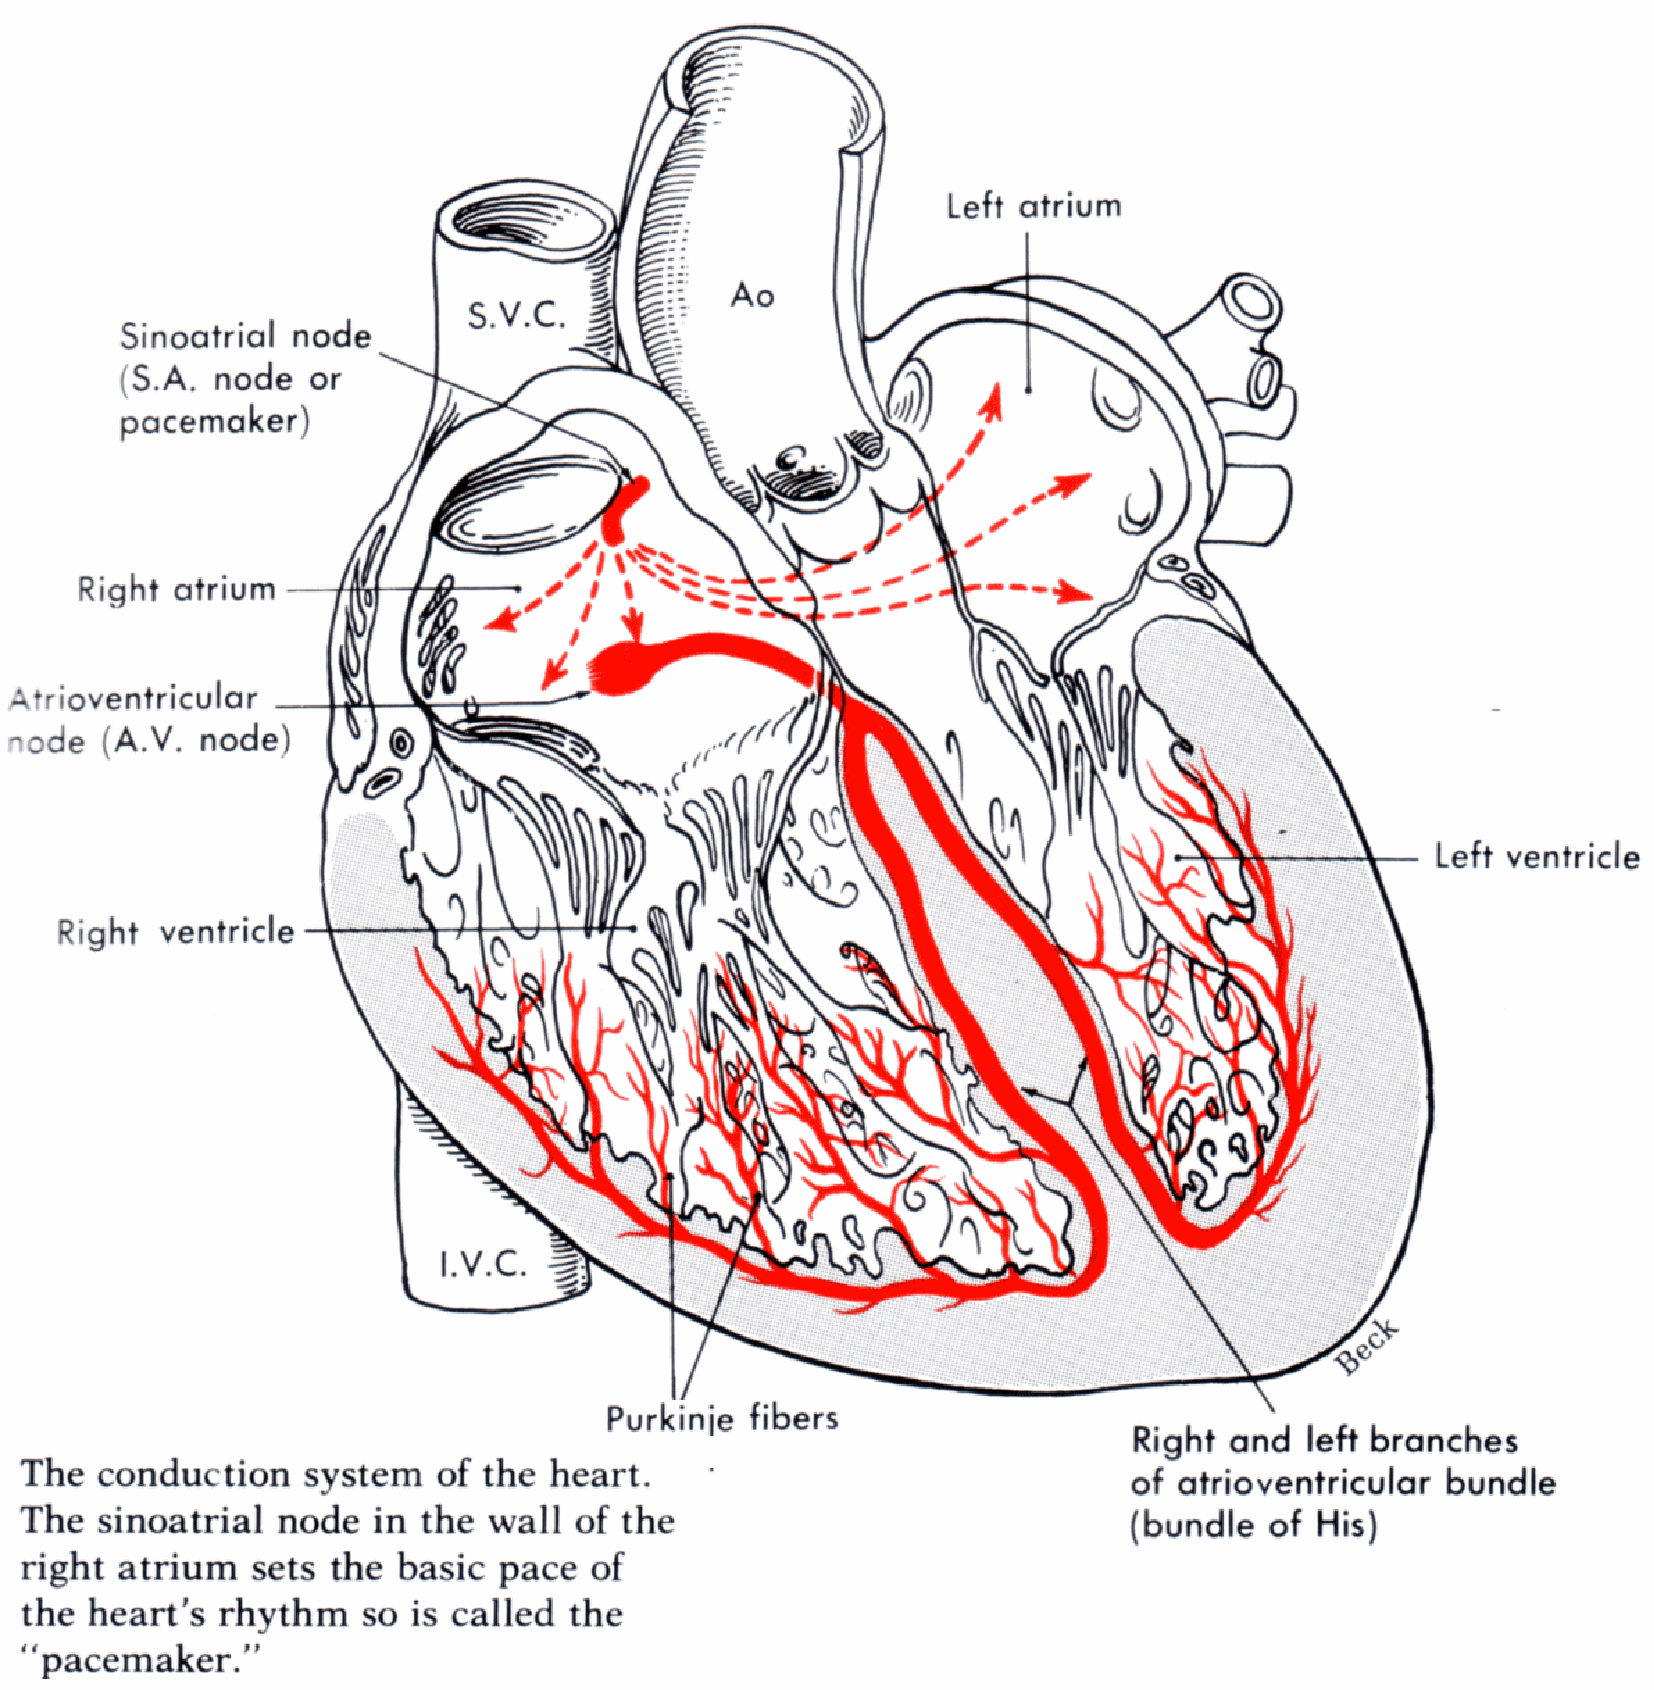
\includegraphics[scale=0.2]{conduction_system.png}
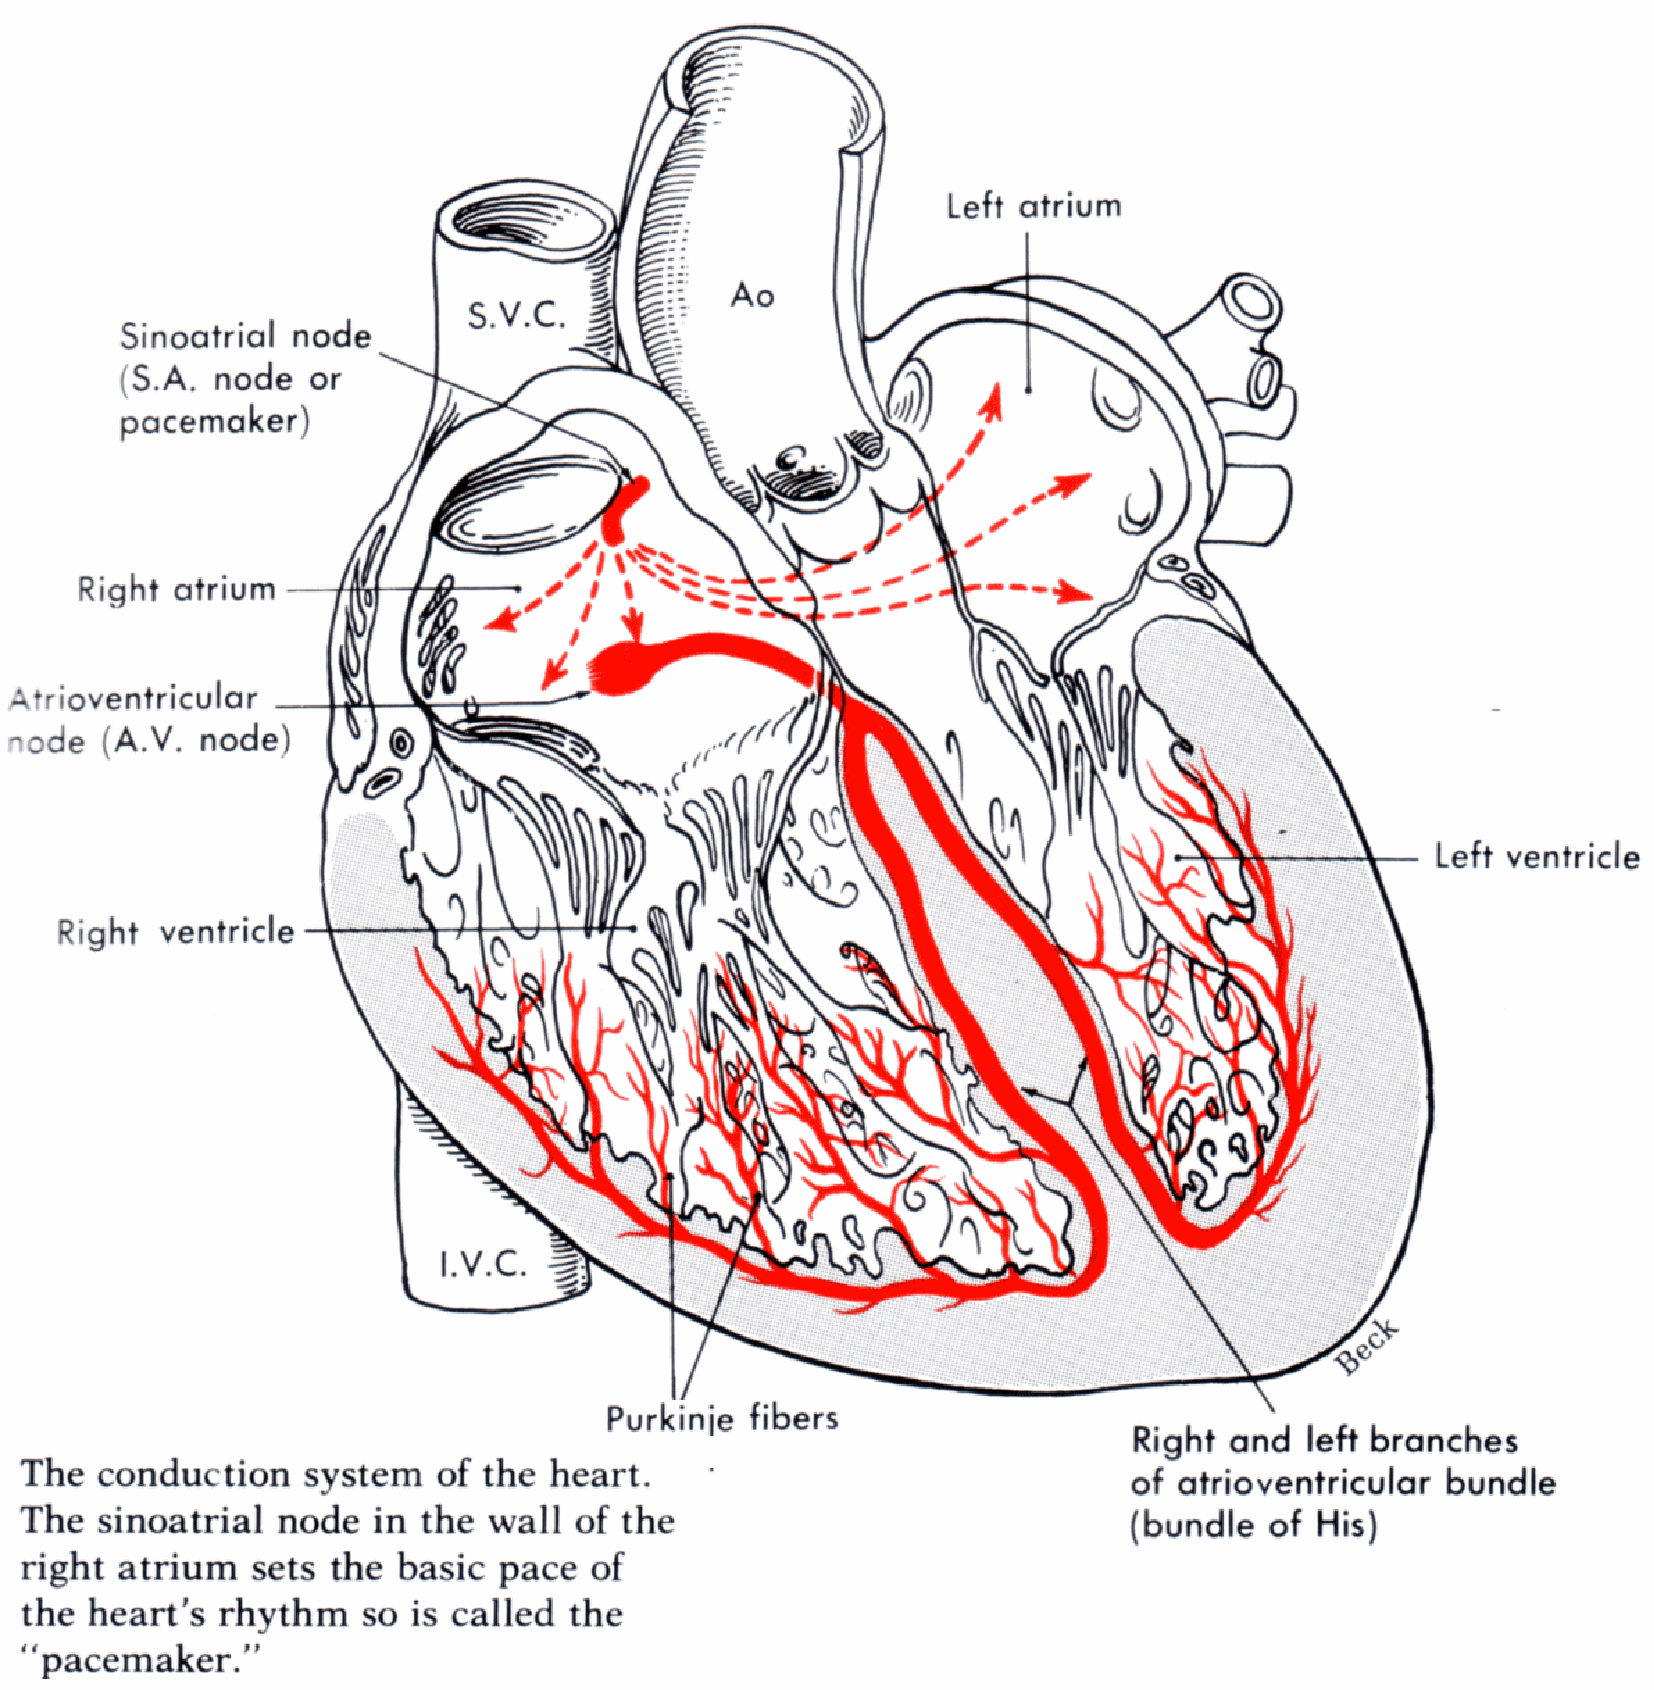
\includegraphics[scale=0.23]{conduction_system.png}
\caption{Scheme of the conduction system of the heart. Figure taken from \cite{amc}}
\label{condsys}
\end{center}
\end{figure}

\newpage

\begin{figure}[H]
\begin{center}
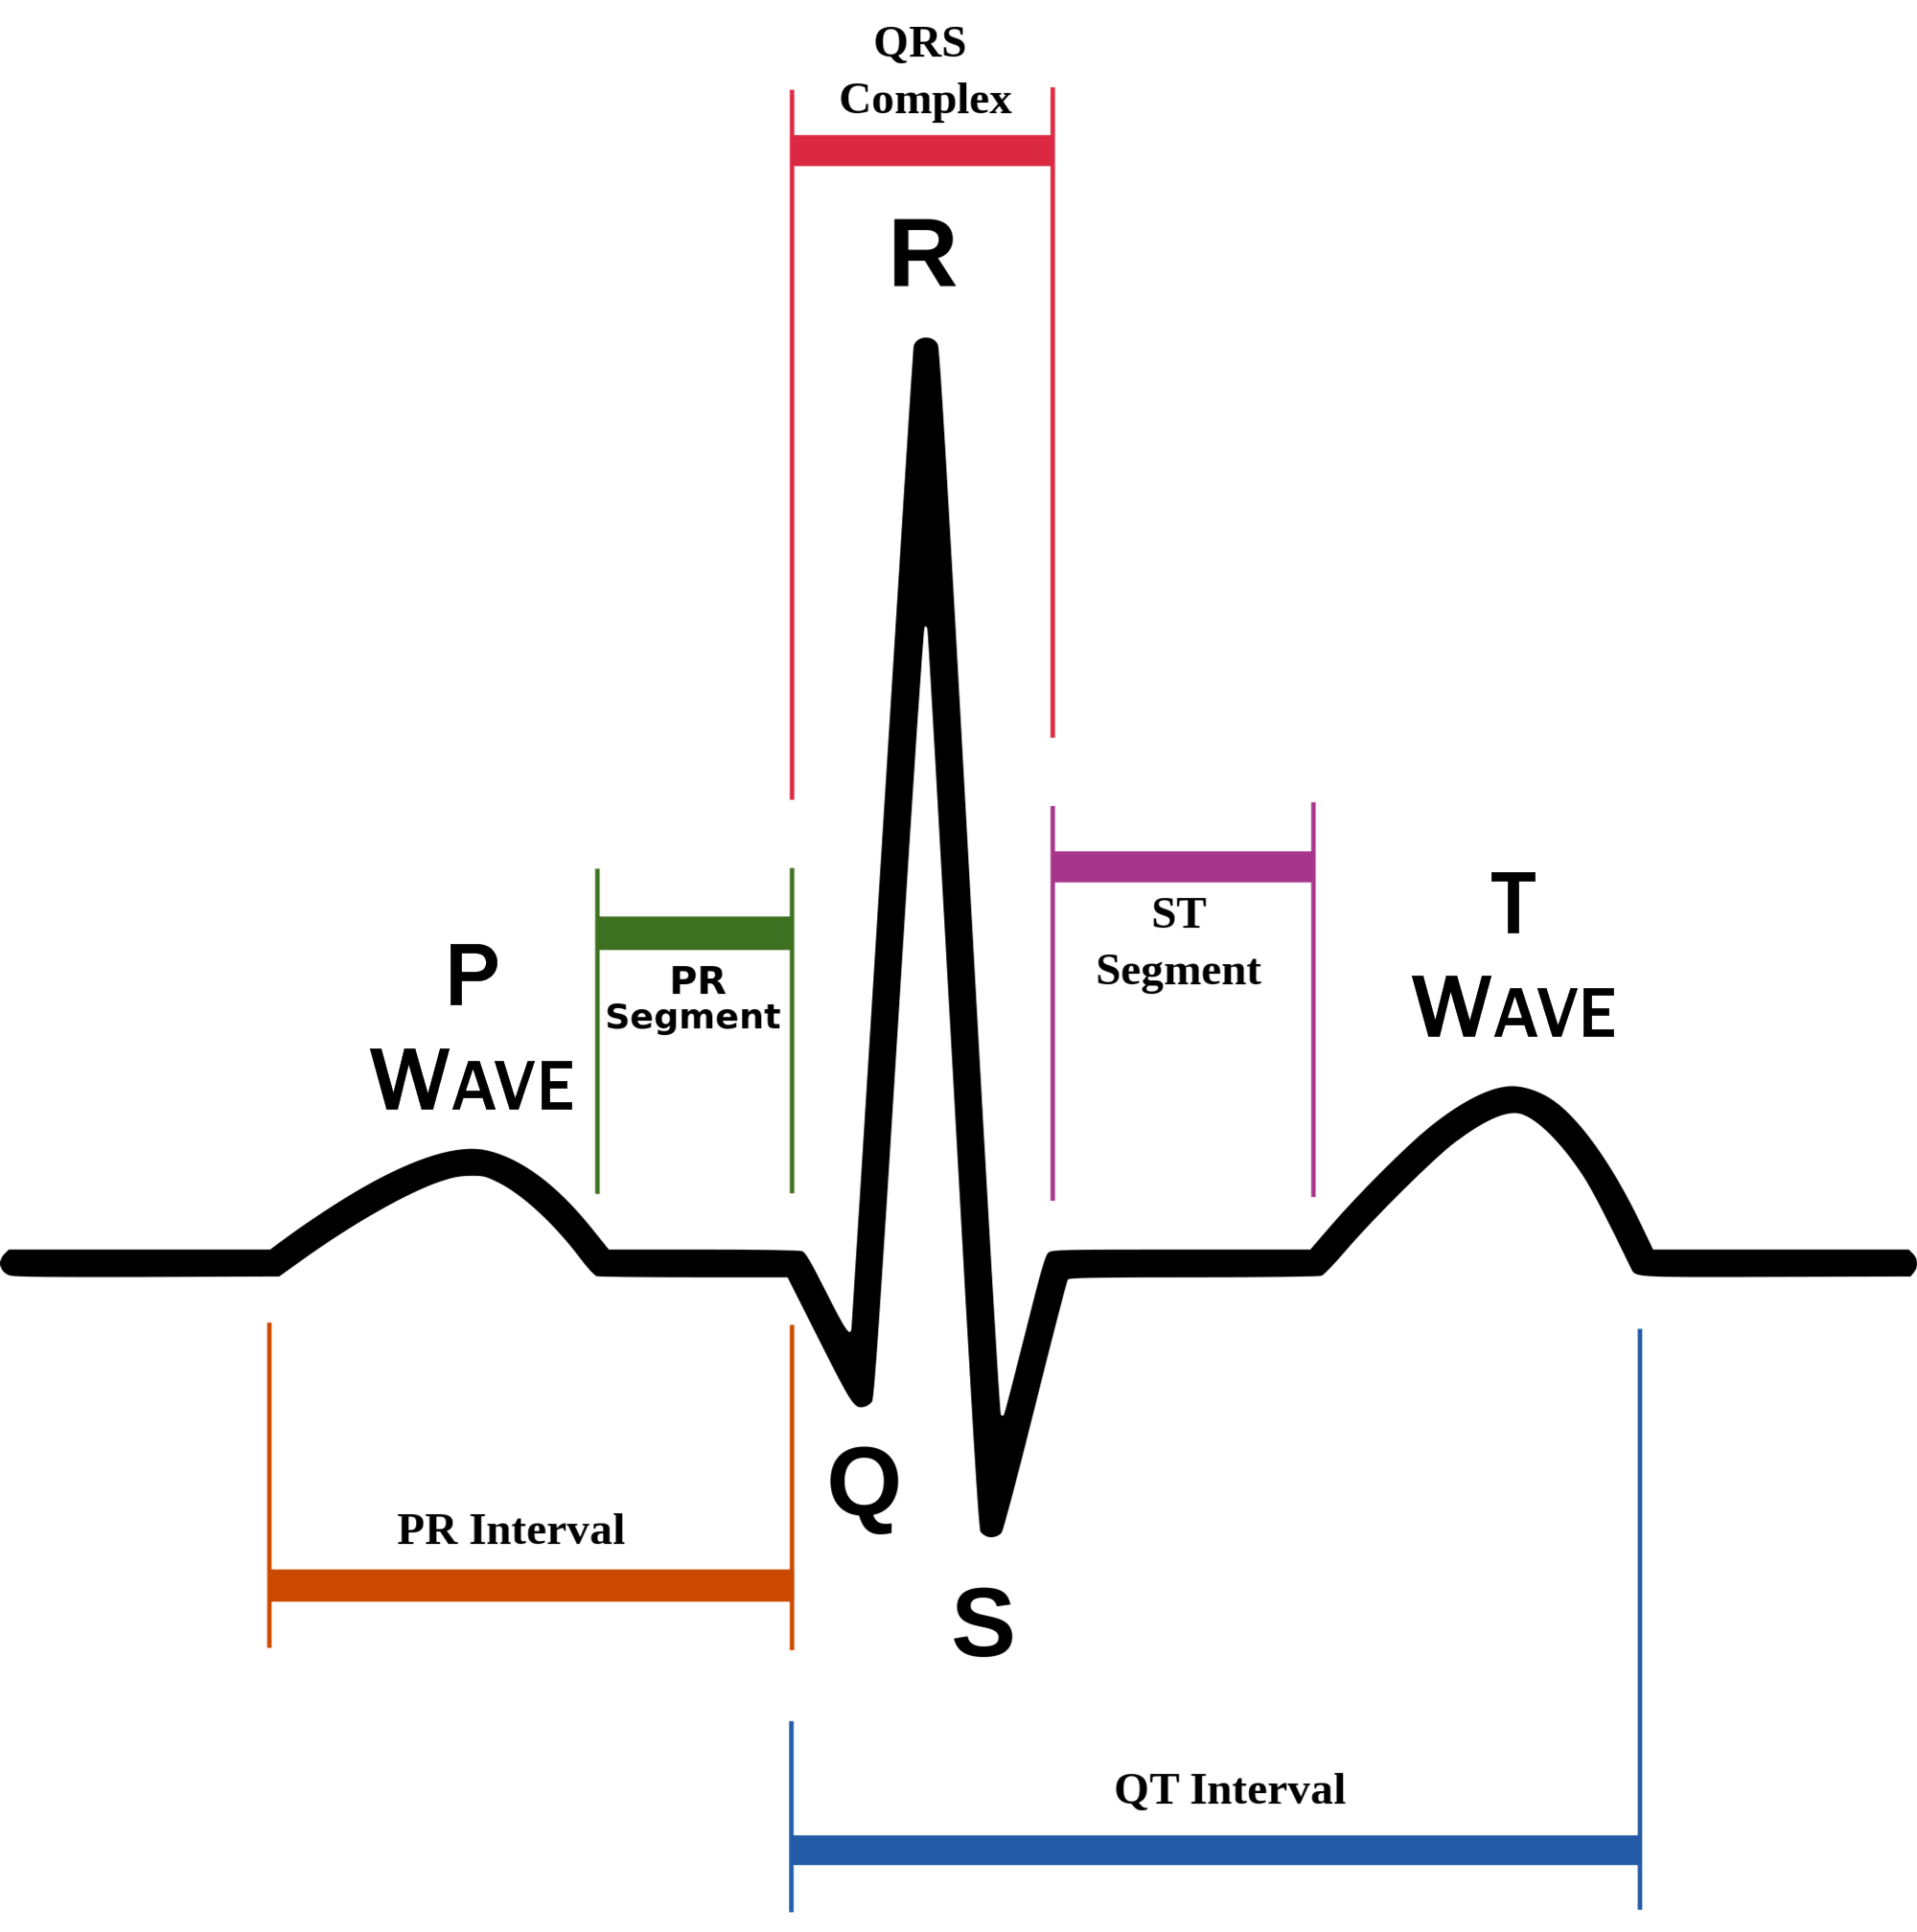
\includegraphics[scale=0.13]{ecg.png}
\caption{ECG trace of a normal heart beat. Figure taken from \cite{afib}}
\label{ecg}
\end{center}
\end{figure}

In AF there is unorganized atrial activity, leading to quivering motion and hence the atria are not able to sustain a healthy pumping rhythm. 
An exemplary ECG trace for AF can be seen in figure \ref{af_ecg}. 
% This is not in itself life threatening but it can dramatically alter the quality of life and increases the risk of suffering a stroke. 
Possible reasons and triggers for this abnormal action potential propagation are stated in the section \ref{AFriskfactor}.

\begin{figure}[H]
\begin{center}
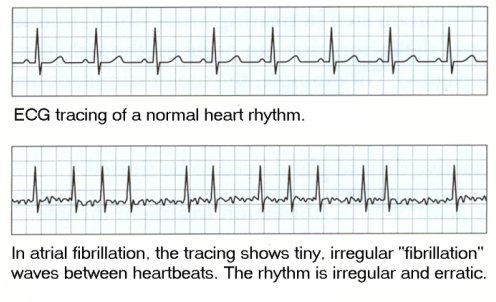
\includegraphics[scale=3]{AF_ECG.png}
\caption{ECG traces for a normal sinus rhythm (upper row) and for an AF patient (lower row). Figure taken from \cite{afib}}
\label{af_ecg}
\end{center}
\end{figure}

\newpage
\subsection{Types of atrial fibrillation}

Based on the duration and presentation of the condition different types of AF are clinically distinguished \cite{ESC10} \cite{CE09} (paroxysmal, 
persistent, long-standing and permanent; fig. \ref{af_types}). 

% \begin{itemize} 
%  \item[] \textbf{First diagnosed AF}: Valid for every patient presenting with AF for the first time. This classification is independent of the 
%  duration, presence or severity of the condition. An episode must last for 30 seconds or longer.
%  \item[] \textbf{Paroxysmal AF}: Recurrent episodes (two or more) of AF which is self-terminating within 48 hours. After this timespan the 
%  likelihood of spontaneous conversion is low.
%  \item[] \textbf{Persistent AF}: Conditions which are present for longer than 7 days or which require cardioversion, independent of the 
%  duration of the episode. 
%  \item[] \textbf{Long-standing persistent AF}: continous episodes of persistent AF present for more than 1 year. Rhythm control 
%  interventions  are carried out in this patient group. 
%  \item[] \textbf{Permanent AF}: classification when the existence of AF is accepted by patient and physician. Restoration and maintenance
%  of sinus rhythm has either failed or has not been attempted. By definition rhythm control interventions are not carried out in these 
%  patient class.  
% \end{itemize}


\begin{figure}[H]
\begin{center}
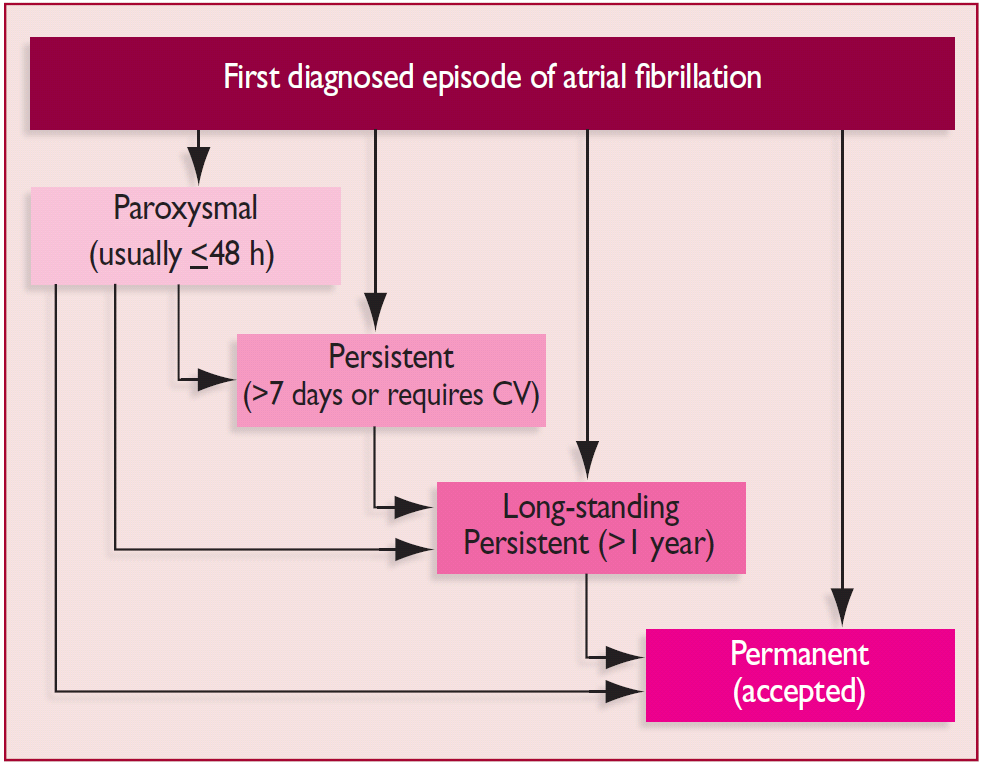
\includegraphics[scale=0.2]{af_types.png}
\caption{Different types of AF. Figure taken from \cite{ESC10}}
\label{af_types}
\end{center}
\end{figure}

Furthermore silent AF may present as any form of the stated AF types. As the name indicates, the condition is asymptomatic and 
hence undiagnosed. It usually manifests as an AF related complication like an ischemic stroke. About one third of people with AF are 
estimated to be unaware of their condition \cite{ESC10}.\newline

Usually AF progresses over time. Starting as short and rare episodes the condition develops into longer and more frequent attacks 
\cite{ESC10}. 

\begin{figure}[H]
\begin{center}
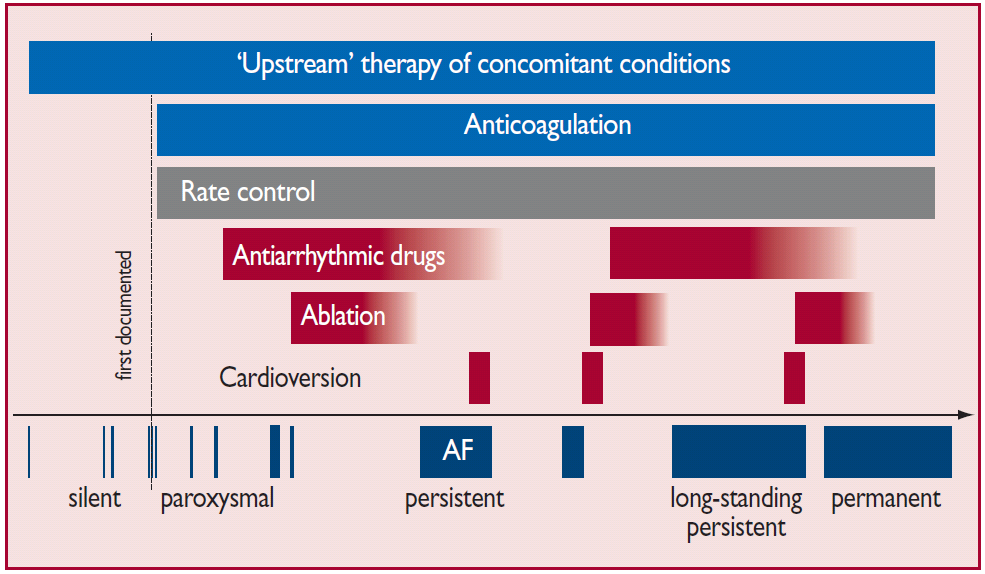
\includegraphics[scale=0.25]{af_over_time.png}
\caption{Typical time course of AF. The dark blue boxes show the different periods of AF. The upper bars indicate possible treatment 
possibilities at the different stages of AF. The light blue boxes represent medication uptake which should prevent the formation of blood 
clots. These medications are recommended in the majority of AF patients. The red boxes indicate system relief therapies while the grey 
boxes represent rate control measures. Figure taken from \cite{ESC10}}
\label{afovertime}
\end{center}
\end{figure}



\subsection{Possible causes for atrial fibrillation and risk factors}
\label{AFriskfactor}

The mechanisms of AF are not yet fully understood. The multifactorial mechanisms may influence and sustain each other. 
Current research indicates that one can distinguish between focal 
mechanisms and multiple wavelets \cite{CE09}. For most patients with paroxysmal AF a localized, focal trigger can be identified. This is 
not the case in patients with persistent or permanent AF, where the multiple wavelet hypothesis is believed to be more accurate.\newline

An identified \textbf{focal trigger} site are the pulmonary veins (PVs). In their benchmark paper Ha\"{\i}ssagurre et al. \cite{Hai98} studied 
45 patients with frequent episodes of AF ( 344 $\pm$ 326 minutes episodes per 24 hours) finding ectopic beats \footnote{beats which arise 
from cells outside the region in the heart muscle ordinarily responsible for impulse formation} originating from the pulmonary veins in 
94 \% of the cases. The underlying mechanism why PVs become arrhythmogenic in some patients while it remains dormant in others is 
still not clear \cite{CE09}. The reason why PVs can become arrhythmogenic at all is based on stages during the embryonic development, in 
which the common PV is incorporated into the left atrium. Immunohistochemical studies have shown that the composition of the PV and the 
smooth-walled portion of the left atrium are identical (see figure \ref{walls}) \cite{CE09} \cite{Dou06}. 

\vspace*{-0.5cm}
\begin{figure}[H]
\begin{center}
% 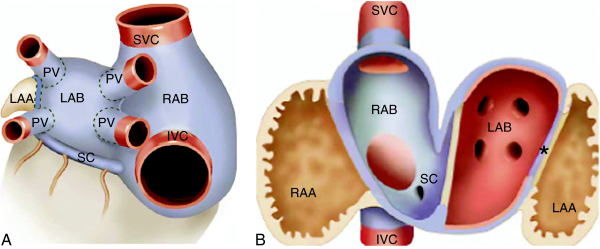
\includegraphics[scale=4.0]{PVatriumTissue.png}
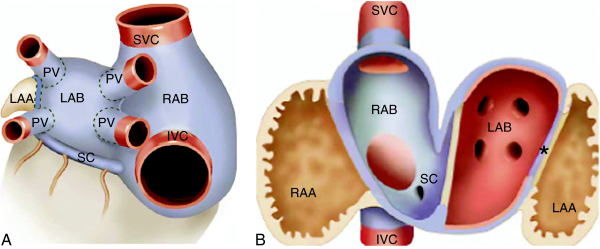
\includegraphics[scale=3.5]{PVatriumTissue.png}
\caption{Schematic depiction of outer side of atrial chambers with pulmonary veins (PV), left atrial appendage (LAA), left atrial body (LAB), 
right atrial body (RAB), superior vena cava (SCV) and inferior vena cava (IVC). LAB and RAB are covered by myocardium (heart muscle tissue) 
with smooth-walled inner aspect (blue), which stretches out over extra cardiac segments of PV (blue area above and below dotted line). 
In A the structures are illustrated from the outside, while B shows the tissue types from the inside of the atria. Figure 
taken from \cite{Dou06}}
\label{walls}
\end{center}
\end{figure}

\vspace*{-0.6cm}
Furthermore, according to the \textbf{multiple wavelet hypothesis} AF is sustained by the continuous propagation of several independent 
wavelets \cite{CE09}. These wavelets are propagating through the muscles of the atria in a chaotic manner. Interference effects between 
various wavelets lead to amplification or cancellation. As long as the number of wave fronts does not decline a certain threshold level AF 
is sustained.\newline

Certain risk factors and indicators for AF can be found in the AF patient group \cite{CE09}. Ageing generally increases the risk of 
developing AF. The reason might be due to age dependent loss of atrial myocardium and the associated conduction disturbances. Hypertension 
is also an age dependent factor which is a risk factor for the incidence of AF as well as AF-related complications such as stroke and 
systematic thromboembolism. 
% Alterations in the heart due to AF are possible and might result in a modified atrial contraction and an 
% increased and irregular ventricular rate. Furthermore abnormalities in the blood flow are evident, resulting e.g. in reduced left atrial 
% appendage flow velocities, an area which is considered the main site of thrombus formation in AF patients \cite{ESC12}. 
Thyroid dysfunction
can be the sole cause of AF and may induce AF related complications. 25 \% of AF patients are obese \cite{Nab09} and 20 \% suffer of 
diabetes mellitus requiring medication. Chronic obstructive pulmonary 
disease (COPD) is found in 10 - 15 \% of AF patients. Nevertheless it is possibly more a marker of general cardiovascular risk then an 
indicator for AF. Chronic renal disease is present in 10 - 15 \% of AF patients and it is suggested that renal failure may increase the 
risk of AF related complications \cite{CE09}. Independent of the stated risk factors AF has also a genetic component, especially 
considering an early onset of AF. In a study carried out by Fox et al. \cite{Fox09} with 2243 offspring participants it was stated that the 
risk of developing AF compared to no parental AF was significantly increased (multivariable-adjusted odds ratio of 1.85, 95 \% confidence 
interval). The results were even stronger when age was limited to an age younger than 75 in parents as well as their offspring 
(multivariable-adjusted odds ratio of 3.23, 95 \% confidence interval). 


\subsection{Treatment modalities}

The treatment modalities for AF have two main goals: to reset the rhythm or to control the ventricular rate and to prevent the formation of blood 
clots \cite{Mayo} \cite{CE09}. The treatment strategy chosen for each individual patient depends on the type of AF and on careful 
consideration of patient individual factors, including the severity of symptoms and potential further heart problems. \newline

Resetting the heart rhythm is the ideal treatment outcome and is carried out by cardioversion, either based on medication (anti-arrhythmic 
drugs) or electrically. In an electrical cardioversion an electrical shock is delivered to the heart, giving the conduction system of the 
heart the possibility to restore its normal activity. Commonly used anti-arrhythmic drugs are e.g. Amiodarone. These drugs have severe side 
effects and can act proarrhythmic, causing also life-threatening ventricular arrhythmias \cite{Mayo}.\newline

If AF can not be converted to a normal heart rhythm through the above stated methods, the ventricular rate needs to be reduced instead. 
Heart rate control can be achieved either by the usage of different medication (e.g. Lanoxib) or by AV node ablation.  
This procedure requires simultaneously the implementation of a pacemaker to establish a heart beat. Hence the atria are still 
fibrillating, so that further medication with anti-arrhythmic medication as well as anticoagulants is required.\newline

For paroxysmal or persistent AF further treatment modalities include the \textbf{Maze procedure} or \textbf{radiofrequency catheter ablation}.\newline

In the \textbf{Maze procedure} scar tissue in the atria is created, inhibiting the propagation of abnormal action potentials. Similar to a maze, 
only a single pathway from the the SA node to the AV node remains accessible for electrical impulses \cite{CTS13}. 
Besides an open chest surgery, the Maze procedure can also be carried out minimal-invasive or with cryotherapy. The success rates as well as 
complications of Maze versus catheter ablation will be studied in the next section.\newline

% in the atria are created by either using a scalpel, radiofrequency energy or cryotherapy. The procedure has 
% very good success rates. In a recently published analysis of 48 studies (involving 3832 patients) it resulted that sinus rhytm was maintained 
% in 83 \% of patients who underwent 
% the maze procedure \cite{CE09} \cite{Kha05}. Nevertheless it requires open heart surgery, making it unsuitable for many patients. It is 
% thus generally reserved to patients who do not respond to other treatment modalities or if it can be combined with other procedures which 
% require heart surgery. \newline

In \textbf{catheter ablation} the main strategy is anatomic based, which means that it is assumed that AF is triggered and sustained by the 
same anatomical sites (the PVs \cite{Hai98}) in the majority of AF patients \cite{CE09}. In radiofrequency ablation a flexible catheter is 
inserted into the patient through a vein close to the groin of the patient and threated into the heart. An electrode on the tip of the catheter 
sends out radiofrequency waves, creating energy and thus heat. This is used to create a 
scar close to the junction between the pulmonary veins and the atria (see figure \ref{af_circ}).\newline

\vspace*{-0.6cm}
\begin{figure}[H]
\begin{center}
% 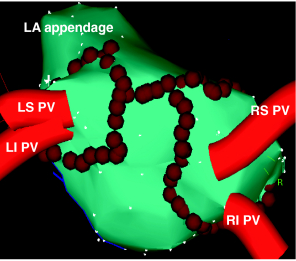
\includegraphics[scale=1.0]{ablation_cut.png}
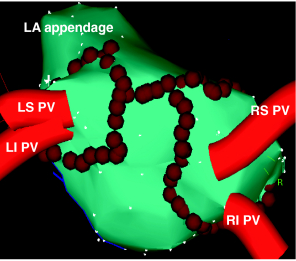
\includegraphics[scale=0.8]{ablation_cut.png}
\caption{Example of circumferential PV ablation. The ablation sites are indicated by the red dots. LI PV: Left inferior pulmonary veins, 
LS PV: left superior pulmonary veins, RI PV: right inferior pulmonary veins, RS PV: right superior pulmonary veins. Figure adapted 
from \cite{Ora06}}
\label{af_circ}
\end{center}
\end{figure}

\vspace*{-0.7cm}

Various ablation techniques exist, including the PV isolation by segmental ostial ablation, circumferential PV ablation (see 
fig. \ref{af_circ}), wide-area circumferential ablation and antral PV isolation \cite{Ora06} \cite{Ora03} \cite{Ouy04}. Antral PV isolation 
and wide-area circumferential ablation was shown to be effective for both patients with paroxysmal and persistent AF \cite{CE09} \cite{Ora03}. 
In a randomized study circumferential PV ablation was found to result in a sinus rhythm in 74 \% of patients with chronic AF \cite{Ora06}. \newline
% Linear ablation is another ablation technique which is either performed in combination with PV circumferential ablation or as stand alone 
% technique \cite{CE09}. The motivation for this procedure is to interrupt reentries.\newline
% \newline

\newpage

Endpoint during PV isolation is to induce a complete electrical isolation of the PVs. This is confirmed by entrance and exit block during 
pacing at multiple sites within the PVs \cite{CE09}. Freedom from recurrent AF can be predicted by 
termination and noninducibility of AF during catheter ablation \cite{Ora02} \cite{Ora06} \cite{Hai05} \cite{Hai04} \cite{Ora04}. Termination 
of AF indicates elimination of all triggers and drivers of AF while noninducibility indicates the absence of residual trggers and drivers 
that may initiate and perpetuate AF \cite{CE09}. Termination is hence not a reliable predictor in patients with paroxysmal AF while 
noninducibility is likely to predict that the patients are going to stay in sinus rhythm (see figure \ref{freedom_recurrence}). 

% \begin{figure}[H]
% \begin{center}
% 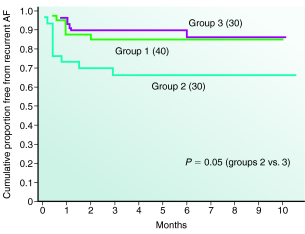
\includegraphics[scale=1.0]{ablation_success_cut.png}
% \caption{Graph showing freedom from symptomatic AF in the absence of antiarrhythmic drug therapy in patients who no longer had inducible AF 
% after circumferential PV ablation (green line, Group 1), who still had inducible or spontaneous AF and did not undergo additional ablation 
% (blue line, Group 2), and who still had inducible AF and underwent additional left atrial ablation (purple line, Group 3). Figure adapted 
% from \cite{Ora04}}
% \end{center}
% \end{figure}

\begin{figure}[H]
\begin{center}
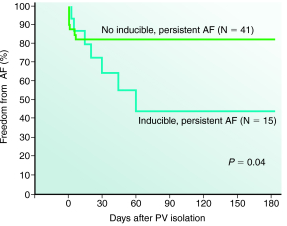
\includegraphics[scale=1]{freedom_recurrence_AF.png}
\caption{Graph showing freedom from AF reocurrance when patients had or had not inducible AF after circumferential PV isolation. Figure adapted 
from \cite{Ora04}}
\label{freedom_recurrence}
\end{center}
\end{figure}


% Alternatively also ablation with cryotherapy can be carried out, in which the heart tissue is not made desolate but rather freezed.\newline

% \newpage

\vspace*{-0.4cm}

Independent of the used procedure, anticoagulants like Warfarin are used in a diversity of patients. In order to establish international 
criteria for risk patients who should uptake anticoagulants, the CHADS$_{2}$-VASc score was defined \cite{ESC12} 
(\textbf{C}ongestive heart failure: 1 point, \textbf{H}ypertension: 1 point, {A}ge ($\geq$ 75): 2 points, \textbf{D}iabetes mellitus: 1 point, 
\textbf{S}troke: 2 points, \textbf{V}ascular disease: 1 point, \textbf{A}ge (65-74): 1 point, \textbf{S}ex (female): 1 point). 
Patients who obtain at least 2 point in the CHADS$_{2}$-VASc score are prescribed anticoagulants. Patients with 1 point might be prescribed 
anticoagulants, alternatively aspirin can be used. Patients with a score of 0 are supposed to only take aspirin \cite{Fle}. The 
CHADS$_{2}$-VASc score has been validated in multiple cohorts \cite{Lip11} \cite{Pot12} \cite{Ole12} \cite{Van11} \cite{Fri12} \cite{Ole11} 
\cite{Bor11}.
% and it was shown that the CHADS$_{2}$-VASc is better then other 
% scores (like the CHADS$_{2}$ score) at identifying low risk patients \cite{Pot12} \cite{Ole12} \cite{Van11} and as good as (or possibly 
% better then) other scores in identifying patients who will develop strokes and thromboembolism \cite{Fri12} \cite{Ole11} \cite{Bor11}. 

\newpage

\subsubsection*{Catheter ablation of AF: success rate and complications}

The FAST trial compared the outcome of catheter ablation and surgical ablation in a randomized study with a small patient population of 124 
patients. 63 patients were treated with catheter ablation, 64 with the invasive surgical ablation. 
The complication rate in catheter ablation was significantly lower (15.9 \% complication rate in catheter ablation versus 34.4 \% in surgical 
ablation
% , driven mainly by procedural complications such as pneumothorax, major bleeding, and the need for pacemaker) 
but at the same time 
the success rate in treatment outcome was reduced (36.5 \% for catheter ablation versus 65.6 \% for surgical ablation after 
12 months) \cite{Boe12}. \newline

In two so-far conducted, nationwide survey the success rates of catheter ablation as a treatment for AF and the resulting complications 
were studied. The first worldwide, multicenter survey was published in 2005 using data obtained from 181 centers in-between 1995 and 2002. 
From these centers 90 stated to have performed 12,830 catheter ablation procedures on 8,745 AF patients. 
It was stated that 52 \% of AF patients undergoing ablation were symptom free without the need of further antiarrhythmic medication and 23.9 \% 
of patients with the need of antiarrhythmic drugs. These success rates were achieved with the requirement of a 
a second (in 24.3 \% of patients) or even third (in 3.1 \% of patients) procedure \cite{Cap05}. Major complication rates were reported in 
6 \% of patients. These complications included 4 early deaths (due to massive cerebral thromboembolism in two patients, extrapericardial PV 
perforation in one patient and unknown reasons in one patient), strokes (in 20 patients), transient ischemic attacks\footnote{"mini-stroke"} 
(in 47 patients) and episodes of tamponade \footnote{fluid collects between the heart muscle and the pericardium, which is the sac containing 
the heart} (in 107 patients). 
In the second worldwide, multicenter survey, which was performed in-between 2003 and 2006 \cite{Cap10} and included 85 catheter ablation 
performing centers (16,309 patients), an improvement in treatment outcome was shown. 
The rate for a successful treatment outcome without the need of further antiarrhythmic medication increased to 
70 \% while the rate with the need of further antiarrhythmic medication decreased to 10 \%, resulting in an overall success rate of 80 \% 
compared to 75.5 \% in the first survey. Concerning the number of needed procedures it was stated that 37.1 \% single treatments were performed, 
59.8 \% dual treatments and 4.1 \% triple treatments.\newline
% When broken down by type of AF, the success rate without antiarrhythmic drugs was 
% 75\% for paroxysmal AF, 65\% for persistent AF, and 63\% for longstanding persistent AF. Major complications 
% occured in 4.5 \% of all patients. These included 25 procedure-related deaths, 37 strokes, 115 transient ischemic 
% attacks, and 213 episodes of tamponade \cite{Cap10}. \newline
% attacks, and 213 episodes of tamponade \cite{Cap10} \cite{Sto}. \newline

% An European survey from 2012 \cite{Arb12} studied the complication rates in catheter ablation. The acute severe complication rates of over 
% 1000 ablation procedures carried out in high-volume centers throughout Europe were reported to be 0.6 \% for stroke, 1.3 \% for tamponade, 
% 1.3 \% for peripheral vascular complications and 2 \% for pericarditis. Similar numbers were reported in an US study \cite{Hoy11} 
% \cite{Cap10}. These informations were obtained from voluntary survey responses and are thus likely to be biased, making the true 
% complications rate possibly higher than stated. In a recent analysis in 4156 patients who had an ablation procedure between 2005 and 2008 
% it was stated that the complication rate was 5 \% and that the rate of hospitalization in the first year after ablation was 38.5 \% 
% (including all possible causes) \cite{Sha12}. Ongoing trials are expected to give more insights in the next years. For now, risk 
% associated with AF ablation needs to be carefully weighed against individual 
% symptomatic benefit \cite{ESC12}. \newline
% 
% All these informations were obtained from voluntary survey responses and are thus likely to be biased, making the true 
% complications rate possibly higher than stated. Ongoing trials are expected to give more insights in the next years \cite{ESC12}.\newline

Recent studies furthermore show that catheter ablation procedures in AF patients are associated with a 
substantial risk of developing silent cerebral embolism \cite{Her13} \cite{Gai10} \cite{Mar13} \cite{Med13} \cite{Schr10} \cite{Lick06}. 
% These findings appear to be independent on the used catheter technology \cite{Sor13} and can not be prevented by oral anticoagulantion 
% therapie \cite{Mar13}. Even though some studies conclude that the lesions created from silent cerebral embolism after catheter ablation are 
% reversible and thus not associated with cognitive deterioration \cite{Sor13} \cite{Her13}, 
Silent cerebral embolism can causes cognitive impairment \cite{Kne08}. A study by Medi et al. \cite{Med13}, which investigated the 
post-operative neurocognitive dysfunction in 150 patients undergoing ablation before and after the treatment, stated a 13 \% - 20 \% incidence 
at long-term follow up of 3 months compared to a control group. \newline

Besides these major complications general disadvantages in the treatment modality of catheter ablation can be concluded. 
Procedures are tedious and can take up to five hours \cite{Jong05}. As fluoroscopy is still the mainstay of catheter imaging in most 
laboratories the patients are furthermore exposed to relatively high X-ray dose \cite{Ber10}. From an socio-economical point of view, 
catheter ablation causes high costs. A total of 13.5 billion Euro are spent on AF patients each year in the EU \cite{Fus06}.\newline

It can be concluded that catheter ablation offers only a limited treatment success rate while major complications and even death due to the 
procedure may occur. Alternative treatment modalities are warranted. Catheter-free ablation using carbon ions could have the potential to 
accurately eliminate arrythmogenic sources at any given cardiac location.

% Concerning the stroke risk in patients after the treatment, numerous recent studies indicate that catheter ablation procedures are 
% associated with a non-negligible risk of silent cerebral embolism \cite{Sor13} \cite{Gai10} \cite{Hai12} \cite{Her13}. XXXX
% This finding is regardless of the exact type of technology used and is mainly produced by the heat XXXX \newline
% 
% Besides major complications in treatment outcome catheter ablation has some further disadvantages which could be improved 
% by a non-invasive treatment modality. The long treatment time of up to five hours \cite{} 
% . resulting in a high dosis 
% exposure to the patient as the procedure is montiored with fluoroscopy (56 $\pm$ 16 min) \cite{}. 
% 
% XXX toedliche nebenwirkungen?
% XXX flouroscopy dauer (56 +/- 16 min)
% XXX op dauer (> 5 Std)
% XXX kosten 


\subsubsection*{Heart irradiation and cardiac radiosurgery}
\label{cardiacradiosurgery}

Target sites in the heart have been irradiated in different procedures. Re-stenosis\footnote{reoccurrence of blood vessel narrowing} after 
angioplasty\footnote{mechanical widening of narrowed blood vessel e.g. with a balloon catheter} for example has been treated with vascular 
brachytherapy \cite{Nat99} \cite{Cot05}. Thereby a minimum dose of 8-16 Gy to a depth of 0.5 mm into the vessel wall was required, while a 
maximum vessel dose did not exceed 32 Gy. Cardiac angiosarcoma, a very rare tumor type in the heart with rare long-term 
survival of the patients, has been treated with carbon ions at the Japanese facility NIRS \cite{Aok04}. A total dose of 64 Gy was given in 16 
fractions in a timeframe of 4 weeks. Follow-up of one and a half year did not show severe side effects.\newline
\newline
Similar to the techniques used in vascular brachytherapy, P\'erez-Castellano et al. \cite{Per06} studied the possibility to use $\beta$-radiation 
as treatment modality for AF. They thereby used a phosphorus-32 source wire centered within a balloon catheter in a study with ten mini swine. 
The delivered dose was calculated to 60 Gy at a depth of 1 mm from the contacting PV wall, resulting in observed PV fibrosis without PV stenosis 
or other side-effects.\newline
\newline
In 2010 a study by Sharma et al. \cite{Sha10} showed that they were able to successfully alter the electrical pathway of the heart 
noninvasively by using stereotactic robotic radiosurgery. In the CyberHeart system cardiac target sites in sixteen mini swine were irradiated 
under general anesthesia. The procedure was as follows. Cardiac CT scans of the anesthetized and intubated mini swine were acquired and an 
electroanatomic mapping \footnote{CARTO system; Biosense-Webster. Three known magnetic sources are used to calculate the orientation 
and position of the catheter tip in 3D, while at the same time the voltage values are determined \cite{bw}} was carried out before the 
irradiation. The voltage was mapped to enable a comparison with the later to be induced electrophysiological effect. Different target sites 
in the heart were chosen. The respiratory motion was compensated by tracking with the CyberKnife Synchrony software, which correlates the 
outside motion of radiopaque markers on the chest wall with the internal motion 
% with a stated accuracy of less than 1.5 mm 
\cite{Ozh08}. For the cardiac motion an ITV approach was chosen. Target volumes were the cavotricuspid isthmus (nine mini swine), 
the AV node (two mini swine), the pulmonary vein - left atrial junction (three mini swine) and the left atrial appendage (two mini swine). 
Dose ranges from 25 Gy to 80 Gy were applied (cavotricuspid isthmus: 25 to 80 Gy, AV node: 40 to 70 days, PV: 38 to 40 Gy and left atrial 
appendage: 32 to 80 Gy). Post irradiation the mini swine were stored at a farm. The follow-up time was dependent on the irradiated target in 
the mini swine (cavotricuspid isthmus: 25 to 89 days, AV node: 15 to 49 days, PV: 35 to 196 days and left atrial appendage: 16 to 33 days). 
In order to assess the irradiation outcome, the animals were again anesthetized and electroanatomically mapped. Afterwards the mini swine 
were euthanized and targets (heart) as well as organs at risk (lung, esophagus) were excised and fixed in formaldehyde. The results of the 
irradiation can be summarized as follows:
The irradiation of the cavotricuspid isthmus evolved during the study, leading to changes in the method of targeting. While initially the 
respiratory and cardiac motion were not compensated for, synchrony and cardiac ITV concepts were later used. While all mini swine 
displayed a reduced conduction across the isthmus, only two animals showed bidirectional block and hence feasibility at 30 days and 40 Gy.   
Targeting the AV node, one animal had to be sacrificed due to pacemaker pocket infection. The other one showed at complete AV block at 49 days, 
after being irradiated with 70 Gy. For the left atrial appendage a decreased voltage was observed at 38 Gy after 33 days. For the left 
pulmonary vein the feasibility was shown as the left atrium showed no local activation in all animals (present from day 35 for all doses) 
(see figure \ref{LA_map}).

\begin{figure}[H]
\begin{center}
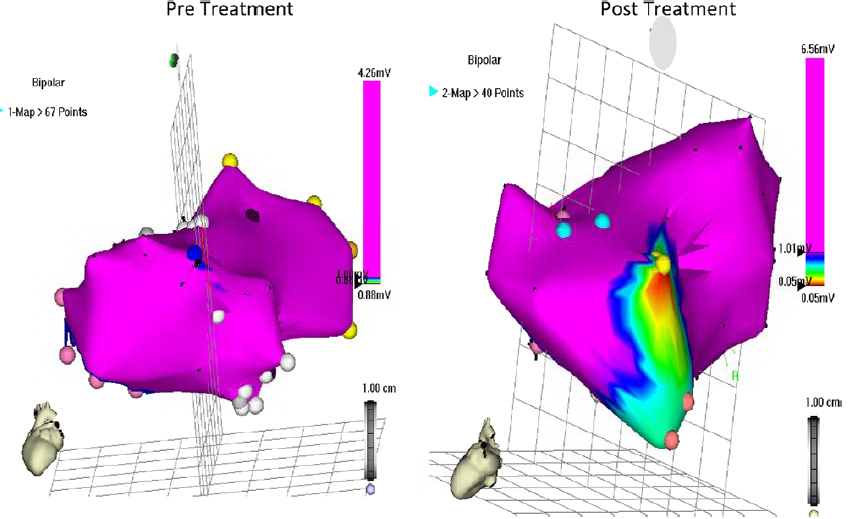
\includegraphics[scale=0.45]{cyberheart_voltagemap.png}
\caption{Electroanatomic voltage map of left atrium before (left side) and after (right side) CyberHeart irradation of PVs. Prior treatment 
no decreased voltage can be observed. Post treatment an area of low-amplitude action potential signals can be seen. Figure from \cite{Sha10}}
\label{LA_map}
\end{center}
\end{figure}

Sharma et al. stated that a dose of 25 Gy or larger was needed to see a change in the electrophysiological properties in the animal model 
after 30 or more days. The dose needed for myocardial fibrosis is also known from other former studies. Fajardo et al. \cite{Faj73} for 
example studied radiation induced fibrosis in rabbit hearts. They observed myocardial fibrosis most often after 2 to 70 days when irradiating 
the rabbits with 20 Gy. Overall Sharma et al. proved that stereotactic radiosurgery has the potential to become a noninvasive treatment 
modality for e.g. atrial fibrillation. \newline
% With the CyberHeart system  treatment times were estimated to lie 
% between 60 and 120 minutes. Lateral scattering of the photons was stated to not exceed 0.05 \% of the target dose in a distance of 1 m 
% from the target, resulting e.g. in a maximum dose of 20 mGy (combined leakage and scatter dose) when irradiating a prescribed dose 
% of 40 Gy. \newline

A subsequent study carried out with the CyberHeart system \cite{Mag11} only targeted the pulmonary veins atrial junction. Two mini swine 
were irradiated with a single fraction treatment of 25 Gy and 35 Gy, respectively and followed for 6 months. It was stated that both animals 
showed circumferential fibrosis, leading to an electrical isolation of the PVs, which was detected with an electroanatomic mapping. 
The mini swine irradiated with 35 Gy showed more extensive necrosis and vasculitis in intramyocardial vessels. It was hence implied that 
25 Gy are sufficient to induce a PV isolation with no major complications in the studied timespan. \newline

In an animal study carried out by Blanck et al. \cite{Bla13} 8 mini swine were irradiated with a single fraction of seven fields with doses 
between 17.5 Gy and 35 Gy. A 5D-ITV concept was applied, hence applying internal margins to the upper right PV accounting for the respiratory 
and heartbeat. Prior treatment electroanatomic mapping was carried out. The animals were followed for 6 months. In this study it was stated 
that a reduction of the electrical signal procession with correlating local transmural fibrosis in the target region was observed at 
doses above 30 Gy. Nevertheless a complete block of the PVs could not be achieved. Stenosis in one branch of 
the PV was observed for the highest applied dose.\newline

All these studies were carried out with photon irradiation. Due to the physical and biological properties of carbon ions (see section \ref{pbb}) 
an improved outcome is expected when treating these deep seated target volumes while aiming to spare the critical organs close by and exposing 
less volume of myocardium to low dose of radiation. The feasibility of this treatment modalities with scanned carbon ions is the aim of this 
work. 


% \subsubsection*{Cardiovascular complications as risk factor for radiation}
% 
% Besides targeting areas in the heart, different radiation processes include the exposure of the heart as an organ at risk to irradiation. 
% Different dose levels are connected to an increased risk of cardiovascular diseases. Total body irraditions as well as highly nonuniformal dose 
% deposition in the treatment of e.g. breast cancer and Hodgkin's lymphoma, are both known to increase the risk of 'radiation-induced' heart 
% diseases (RIHD).\newline
% \newline
% Information on the consequence of total body irradiation (TBI) was demonstrated in the Japanese atomic bomb survivors. In this population the 
% mortality of cardiovascular diseases was drastically increased more than 40 years after exposure \cite{Bak11} \cite{Pre03}. The dose deposition 
% in an atomic bomb was determined as an acute dose of 1-2 Gy. The mortality risk increased by 17 \% per Gy after TBI between 0 and 4 Gy.\newline
% \newline
% In the mid 1960s it has been recognized that cancer radiotherapy can cause damage to the heart and the pericardium\footnote{double-walled 
% sac containing the heart} \cite{Coh67}. Ecspecially irradiation of breast cancer and Hodgkin's lymphoma\footnote{cancer of the 
% lymphatic system} patients yield highly nonuniformal dose depositions in the cardiac region. Various studies analyse the potential increase of 
% RIHD as a health concern in these patient groups. RIHD can include a variety of diseases, depending on the component 
% involved \cite{Jaw13}. Particular increase exist in coronary artery disease, congestive heart failure, valvular heart diseases, pericardial 
% disease, conduction abnormalities and sudden cardiac death \cite{Ale03} \cite{Swe07} \cite{Ng02} \cite{Hei03} \cite{Wet09} (1-5 in Jaw13). 
% It is stated that cardiovascular diseases are the most common nonmalignant death cause in breat cancer and Hodgkin's lymphoma patients treated 
% with radiotherapy \cite{Ale03} \cite{Ng11} \cite{Hop97} \cite{Pat11} \cite{Jaw13} \cite{Lan13} (+6-8 in Jaw13). 
% As these radiation effects are late effects, usually appearing after the second or third decade after radiotherapy 
% \cite{Ale03} \cite{Swe07} \cite{Wat09} \cite{Cas11} (+ 10 in Jaw13) many of the now studied 
% patients were irradiated with now out-dated protocols and fractionation schemes \cite{Jaw13}. Improved radiation techniques have been 
% developed over the years to minimise the radiation to the heart. Nevertheless the residual risk remains unclear.\newline
% \newline
% The largest study exploring the impact of nonmalignant death causes for breast cancer patient was carried out by the Early Breast Cancer 
% Trialists Collaborative Groupt \cite{Ear00} (24 in Jaw13). The study showed that the 20 year survival 69.5 \% among those who underwent 
% radiotherapy while it was 73.8 \% in the control group (in absence of any cancer patient deaths). Comparing the benefit of radiotherapy 
% to the late-effects it was stated that the annual mortality rate from breast cancer was decreased by 13 \%  through radiotherapy, while the 
% mortality by other causes was increased by 21 \%, again by using now out-dated and as suboptimal considered radiation techniques and 
% protocols. Radiotherapy of left-sided versus right-sided breast cancer was also used as an indicator for risk of mortality from 
% cardiovascular diseases \cite{Bak11}. Data analysis of the U.S. Surveillance Epidemiology and End Result (SEER) cancer registries \cite{Dar05}
% (28 in Bak11) resulted in an mortality ratio of 1.6 in left-sided versus right-sided incidences. It was furthermore stated that the 
% risk increased over time (1.04 for less than 5 years after diagnosis, to 1.1 for 5-10 years, to 1.37 for 10-15 years and to 1.53 for 15 years 
% or more). A recent population-based control study from Darby et al. \cite{Dar13} (eigenes Paper) dealed with the risk of breast cancer patients 
% developing ischemic heart diseases. The study included 2168 women who underwent radiotherapy for breast cancer between 1958 and 2001 in Sweden 
% and Denmark (963 women with major coronary events and 1205 control patients). It was stated that major coronary events increased linearly with 
% the mean dose to the heart by 7.4 \% per Gy, whereas no threshold was observed. This increase was observed within 5 years after radiotherapy and 
% continued up to 30 years.\newline
% \newline
% Hodgkin's lymphoma is the most common cancer in young adults. It has high survival rates if recognized at an early stage (approaching 85 \% 
% for 5 years) \cite{Jaw13}. Cardiovascular diseases, with Myocardial infarction being the most common, account for 25 \% of nonmalignant death 
% causes in the cured patient group after radiotherapy \cite{Swe07} \cite{Lee00} \cite{Rij08} \cite{Gla98} (+15,17,18 in Jaw13). Up to 88 \% 
% of the treated patients demonstrate asymptomatic cardiac abnormalities \cite{Car07} (20 in Jaw13).\newline
% \newline
% It can be concluded that there is compelling evidence that radiotherapy in the chest area can increase the risk of the patient to suffer 
% a radiation induced heart disease. The development depends on a variety of factors like e.g. the total dose 
% radiation, the fraction dose used per day, the area of heart exposed to radiation and the use of certain chemotherapeutic drugs \cite{Gay05} \cite{Car07} 
% \cite{Jon07} (+ 16,und 61 in Jaw13). The risk becomes apparent in doses higher than 30 Gy \cite{Lan13}, nevertheless smaller doses might 
% cause similar effects and no apparent threshold dose was so far observed. Latence time of at least 5 years after radiotherapy are often 
% stated and continue up to three decades post treatment. Furthermore many risk factors for cancer are shared risk factors of 
% developing cardiovascular diseases, like e.g. age, an increased body mass index, inactivity and substance abuse (smoking, drinking) 
% \cite{Lan13}, which might lead to a possible accerleration of RIHD. 
% 


\begin{thebibliography}{9999999}
 \bibitem[ACC06]{ACC06}{Bonow RO et al: ACC/AHA 2006 Guidelines for the Management of Patients With Valvular Heart Disease; J. Am. Coll. Cardiol.; 48(3); 2006}
 \bibitem[afib]{afib}{Atrial fibrillation Resources for patients, a-fib.com}
 \bibitem[Ahl80]{Ahl80}{Ahlen SP: Theoretical and experimental aspects of the enery loss of relativistic heavily ionizing particles; Rev.Mod.Phys; 52(1); 121; 1980}
 \bibitem[Alp98]{Alp98}{Alpen EL: Radiation Biophysics; Academic Press; 2nd edition; 1998}
 \bibitem[Ama04]{Ama04}{Amaldia U: CNAO - the Italian centre for light ion therapy; Radiotherapy and Oncology; 73(Supplement 2); 191-201; 2004}
 \bibitem[amc]{amc}{Arthur's Medical Clipart, arthursclipart.org}
 \bibitem[Aok04]{Aok04}{Aoka Y, Kamada T, Kawana M, Yamada Y, Nishikawa T, Kasanuki H and Tsujii H: Primary cardiac angiosarcoma treated with carbon-ion radiotherapy; Lancet Oncol; 5; 636-638; 2004}                       
% %  \bibitem[Arb12]{Arb12}{Arbelo E, Brugada J, Hindricks G, Maggioni A, Tavazzi L, Vardas P, Anselme F, Inama G, Jais P, Kalarus Z, Kautzner J, Lewalter T, Mairesse G, Perez-Villacastin J, Riahi S, Taborsky M, Theodorakis G, Trines S; on behalf of the Atrial Fibrillation Ablation Pilot Study Investigators. ESC-EURObservational research programme: the atrial fibrillation ablation pilot study, conducted by the European Heart Rhythm Association. Europace 2012;14:1094-1103}
 \bibitem[Bar63]{Bar63}{Barkas H.W.: Nuclear Research Emulsions; Vol.I; Academic Press New York and London; 1963}
 \bibitem[Ben98]{Ben98}{Benjamin EJ, Wolf PA, D?Agostino RB, Silbershatz H, Kannel WB, Levy D. Impact of atrial fibrillation on the risk of death: the Framingham Heart Study.; Circulation.; 98; 946?952; 1998}
 \bibitem[Ber05]{Ber05}{Bert C, Metheany KG, Doppke K, Chen GT: A phantom evaluation of a stereovision surface imaging system for radiotherapy patient setup; Medical Physics; 32(9); 2753-2762; 2005}
 \bibitem[Ber06]{Ber06}{Bert C: Bestrahlungsplanung f\"ur bewegte Zielvolumina in der Tumortherapie mit gescanntem Kohlenstoffstrahl; Dissertation; TU Darmstadt; 2006}
 \bibitem[Ber07]{Ber07}{Bert C, Saito N, Schmidt A, Chaudhri N, Schardt D and Rietzel E: Target motion tracking with a scanned particle beam; Medical Physics; 34(12); 4768-4771; 2007}
 \bibitem[Ber07b]{Ber07b}{Bert C and Rietzel E: 4D treatment planning for scanned carbon ion beams; Radiat. Oncol; 2(24); 2007}
 \bibitem[Ber08]{Ber08}{Bert C, Groezinger SO and Rietzel E: Quantification of interplay effects of scanned particle beams and moving targets; Phys. Med. Biol.; 53(9); 2253-2265; 2008}
 \bibitem[Ber09]{Ber09}{Bert C, Gemmel A, Saito N and Rietzel E: Gated irradiation with scanned particle beams; Int. J. Radiat. Oncol. Biol. Phys.; 73(4); 1270-1275; 2009}
 \bibitem[Ber09b]{Ber09b}{Bert C, Gemmel A, Chaudhri N, L\"uechtenborg R, Saito N, Durante M and Rietzel E: Rescanning to mitigate the impact of motion in scanned particle therapy; GSI Scientific Report; 397; 2008}
 \bibitem[Ber10]{Ber10}{Bert C, Gemmel A, Saito N, Chaudhri N, Schardt D, Durante M, Kraft G and Rietzel E: Dosimetric precision of an ion beam tracking system; Radiat. Oncol.; 5(1); 61; 2010}
% %  \bibitem[Ber10b]{Ber10b}{Bert C, Moosdorf R, Vogt S, Zink K: Behandlung von Herzrhythmusst\"orungen und Herzinsuffizienz durch einen gescannten Ionenstrahl; Innovationswettbewerb zur F\"orderung der Medizintechnik; BASIS Antrag; 2010}
 \bibitem[Bet30]{Bet30}{Bethe H: Zur Theorie des Durchgangs schneller Korpuskularstrahlung durch Materie; Annalen der Physik; 5(5); 325-400; 1930}
 \bibitem[Bla13]{Bla13}{Blanck O, Bode F, Gebhard M, Hunold P, Brandt S, Bruder R, Schweikard A, Grossherr M, Rades D and Dunst J: Radiochirurgisch erzeugte L\"asionen im Antrum der Pulmonarvenen: Vorl\"aufige Ergebnisse im Tiermodell und m\"ogliche Implikationen f\"ur die Behandlung von Vorhofflimmern; DEGRO 2013}
 \bibitem[Blo33]{Blo33}{Block F: Bremsverm\"ogen von Atomen mit mehreren Elektronen; Zeitschrift der Physik A Hadrons and NUclei; 81(5); 285-321; 1933}
 \bibitem[Boe12]{Boe12}{Boersma LV et al: Atrial fibrillation catheter ablation vs. surgical ablation treatment (FAST): a 2-center randomized clinical trial; Circulation 125; 23-30; 2005}
 \bibitem[Bor11]{Bor11}{Boriani G et al: Italian AT-500 Registry Investigators. Improving stroke risk stratification using the CHADS$_{2}$ and CHADS$_{2}$-VASc risk score in patients with paroxysmal atrial fibrillation by continous arrhythmia burden monitoring; Stroke 42; 1768-1770; 2011}
 \bibitem[Bor40]{Bor40}{Bohr N: Scattering and stopping of fission fragments; Phys.Rev.; 58(7); 654-655; 1940}
 \bibitem[Bro10]{Bro10}{Brock KK: Results of multi-institution deformable registration accuracy study (midras); Int. J. Radiat. Oncol. Biol. Phys.; 76(2); 538-596; 2010}
 \bibitem[Buc05]{Buc05}{Bucci MK, Bevan A and Roach M: Advances in radiation therapy: Conventional to 3D, to IMRT, to 4D, and beyond; CA: A Cancer Journal for Clinicians; 55(2); 117-134; 2005}
 \bibitem[bw]{bw}{http://www.biosensewebster.com/carto3.php}
 \bibitem[Cap05]{Cap05}{Cappato R et al: Worldwide Survey on the Methods, Efficacy, and Safety of Catheter Ablation for Human Atrial Fibrillation; Circulation 111; 1100-1105; 2005}
 \bibitem[Cap10]{Cap10}{Cappato R, Calkins H, Chen SA, Davies W, Iesaka Y, Kalman J, Kim YH, Klein G, Natale A, Packer D, Skanes A, Ambrogi F, Biganzoli E: Updated Worldwide Survey on the Methods, Efficacy, and Safety of Catheter Ablation for Human Atrial Fibrillation; Circulation: Arrhythmia and Electrophysiology 3; 32-38; 2010} 
 \bibitem[CE09]{CE09}{Cardiac Electrophysiology: From Cell to Bedside, Zipes and Jalife, Saunders Elsevier, 5th Edition, 2009}
 \bibitem[Cha76]{Cha76}{Chatterjee A and Schaefer HJ: Microdosimetric structure of heavy ion tracks in tissue; Radiat. Environ. Biophys.; 13; 215-227; 1976}
 \bibitem[Chu93]{Chu93}{Chu WT, Ludewigt BA, Renner TR: Instrumentation for treatment of cancer using protons and light-ion beams; Accelerator and Fusion Research Division; LBL-33403 UC-406 preprint; 1993}
 \bibitem[Com10]{Com10}{Combs SE, J\"akel O, Haberer T, Debus J: Particle therapy at the Heidelberg Ion Therapy Center (HIT) - Integrated research-driven university-hospital-based radiation oncology service in Heidelberg, Germany; Radiotherapy and Oncology; 95(1); 41-44; 2010}
 \bibitem[Com11]{Com11}{Combs SE, Habermehl D, Ganten T, Schmidt J, Edler L, Burkholder I, J\"akel O, Haberer T and Debus J: Phase i study evaluating the treatment of patients with hepatocellular carcinoma (HCC) with carbon ion radiotherapy: The PROMETHEUS-01 trial; BMC Cancer; 11; 2011}
 \bibitem[Cot05]{Cot05}{Cotton JM, Rance K, Patil A and Thomas MR: Intracoronary brachytherapy for the treatment of complex in-stent restenosis; Heart; 91; 231-231; 2005}
 \bibitem[CTS13]{CTS13}{cts.usc.edu/mazeprocedure.html; Cardiothoracic surgery, University of Southern Carolina Keck School of Medicine; 2013}
 \bibitem[Dou06]{Dou06}{Douglas YL, Jongbloed MR, Gittenbergerde Groot AC et al: Histology of vascular myocardial wall of left atrial body after pulmonary venous incorporation; Am J Cardiol 97; 662-670; 2006}
 \bibitem[Ele12]{Ele12}{Eley J, Graeff C, L\"uchtenborg R, Durante M, Howell R, Newhauser W and Bert C: 4D Optimization for Scanned Ion Beam Tracking Therapy for Moving Tumors; Medical Physics; 39(6); 3970; 2012}
 \bibitem[Eng11]{Eng11}{Engelsman M and Bert C: Precision and Uncertainties in Proton Therapy for Moving Targets; in Paganetti H: Proton Therapy Physics; Taylor \& Francis; 2011}
 \bibitem[Eva08]{Eva08}{Evans PM: Anatomical imaging for radiotherapy; Physics in Medicine and Biology; 53(12); 151-191; 2008}
 \bibitem[ESC10]{ESC10}{ESC Guidlines for the management of atrial fibrillation: The task force for the Management of Atrial Fibrillation of the European Society of Cardiology (ESC); European Heart Journal 31; 2369-2429; 2010}
 \bibitem[ESC12]{ESC12}{2012 focused update of the ESC Guidlines for the management of atrial fibrillation: An update of the 2010 ESC Guidlines for the management of atrial fibrillation; European Heart Journal; 2012}
 \bibitem[Faj73]{Faj73}{Fajardo LF and Stewart JR: Pathogenesis of radiation-induced myocardial fibrosis; Laboratory Investigation; 29; 2; 244; 1973}
 \bibitem[Fle]{Fle}{http://flexikon.doccheck.com/de/CHA2DS2-VASc-Score}
 \bibitem[Fok04]{Fok04}{Fokdal L et al: Impact of changes in bladder and rectal filling volume n organ motion and dose distribution of the bladder in radiotherapy for urinary bladder cancer; Int. J. Radiat. Oncol. Biol. Phys.; 59(2); 436-444; 2004 }
 \bibitem[Fox09]{Fox09}{Fox CS et al: Parental atrial fibrillation as a risk factor for atrial fibrillation in offspring; JAMA 291; 2851-2855; 2004}
 \bibitem[Fri12]{Fri12}{Friberg L et al: Evaluation of risk stratification schemes for ischemic stroke and bleeding in 182 678 patients with atrial fibrillation: the Swedish Atrial Fibrillation Cohort study; Eur Heart J 33; 1500-1510; 2012}
 \bibitem[Frie13]{Frie13}{Friedrich T, Gr\"un R, Scholz U, Elsässer T, Durante M, Scholz M.: Sensitivity analysis of the relative biological effectiveness predicted by the local effect model; Phys Med Biol.; 58(19); 6827-6849; 2013}
 \bibitem[Fur07]{Fur07}{Furukawa T, Inaniwa T, Sato S, Tomitani T, Minohara S, Noda K and Kanai T: Design study of a raster scanning system for moving target irradiation in heavy-ion radiotherapy; Medical Physics; 34(3); 1085-1097; 2007}
 \bibitem[Fus06]{Fus06}{Fuster V, Ryden LE, Cannom DS et al: ACC/AHA/ESC 2006 guidelines for the management of patients with atrial fibrillation; Europace; 8(9); 651-745; 2006}
 \bibitem[Gai10]{Gai10}{Gaita F, Caponi D, Pianelli M, Scaglione M, Toso E, Cesarani F, Boffano C, Gandini G, Valentini MC, De Ponti R, Halimi F, Leclercq JF: Radiofrequency catheter ablation of atrial fibrillation: A cause of silent thromboembolism? Magnetic resonanceimaging assessment of cerebral thromboembolism in patients undergoing ablation of atrial fibrillation; Circulation;122:1667-1673; 2010}
 \bibitem[Gem11]{Gem11}{Gemmel A, Rietzel E, Kraft G, Durante M and Bert C: Calculation and experimental verification of the RBE-weighted dose for scanned ion beams in the presence of target motion; Phys Med Biol.;56(23); 2011}
 \bibitem[Gra12]{Gra12}{Graeff C, Durante M and Bert C: Motion mitigation in intensity modulated particle therapy by internal target volumes covering range changes; Med. Phys.; 39; 6004?6013; 2012}
 \bibitem[Gra13]{Gra13}{Graeff C, Constantinescu A, L\"uchtenborg R, Durante M and Bert C: Multigating: 4D optimized beam tracking in scanned ion beam therapy; TCRT Express; submitted}
 \bibitem[Gro04]{Gro04}{Groezinger SO: Volume conformal irradiation of moving target volumes with scanned ion beams; Dissertation; TU Darmstadt; 2004}
 \bibitem[Hab93]{Hab93}{Haberer T et al: Magnetic Scanning System for Heavy Ion Therapy; Nucl.Inst \& Meth. in Phys. Res.; A330; 296-305; 1993}
 \bibitem[Hai98]{Hai98} {Ha\"{\i}ssagurre M, Jais P, Shah DC et al: Spontaneous initiation of atrial fibrillation by ectopic beats originating in the pulmonary veins; N Engl J Med 339; 659-666; 1998}
 \bibitem[Hai04]{Hai04}{Ha\"{\i}ssaguerre M, Sanders P, Hocini M, et al: Changes in atrial fibrillation cycle length and inducibility during catheter ablation and their relation to outcome. Circulation  2004; 109:3007-3013}
 \bibitem[Hai05]{Hai05}{Ha\"{\i}ssaguerre M, Hocini M, Sanders P, et al: Catheter ablation of long-lasting persistent atrial fibrillation: Clinical outcome and mechanisms of subsequent arrhythmias. J Cardiovasc Electrophysiol  2005; 16:1138-1147} 
% %  \bibitem[Hain12]{Hain12}{Haines DR, Stewart MT, Dahlberg S, Barka ND, Condie C, Fiedler GR, Kirchhof NA, Halimi F, Deneke T: Microembolism and Catheter Ablation I : A Comparison of Irrigated Radiofrequency and Multielectrode-phased Radiofrequency Catheter Ablation of Pulmonary Vein Ostia; Circ Arrhythm Electrophysiol.; 2013}
 \bibitem[Hal06]{Hal06}{Hall EJ and Giaccia AJ: Radiobiology for the Radiologist; Lippincott Williams \& Wilkins; 6th Edition; 2006}
 \bibitem[Han99]{Han99}{Hanley J et al: Deep inspiration breath-hold technique for lung tumors: the potential value of target immobilisation and reduced lung density in dose escalation; Int. J. Radiat. Oncol. Biol. Phys.; 45(3); 603-611; 1999}
 \bibitem[Has06]{Has06}{Hashimoto T et al: Repeated proton beam therapy for hepatocellular carcinoma; Int. J. Radiat. Oncol. Biol. Phys.; 65(1); 196-202; 2006}
 \bibitem[Her13]{Her13}{Herm J et al: Neuropsychological Effects of MRI-Detected Brain Lesions after Left Atrial Catheter Ablation for Atrial Fibrillation: Long Term Results of the MACPAF Study; Circ Arrhythm Electrophysiol.; 2013}
 \bibitem[Hof03]{Hof03}{Hof H et al: Stereotactic single-dose radiotherapy of stage I non-small cell lung cancer (nsclc); Int. J. Radiat. Oncol. Biol. Phys.; 56(2); 335-341; 2003}
% %  \bibitem[Hoy11]{Hoy11}{Hoyt H, Bhonsale A, Chilukuri K, Alhumaid F, Needleman M, Edwards D, Govil A, Nazarian S, Cheng A, Henrikson CA, Sinha S, Marine JE, Berger R, Calkins H, Spragg DD. Complications arising from catheter ablation of atrial fibrillation: temporal trends and predictors. Heart Rhythm 2011;8:1869 – 1874.}
 \bibitem[ICRU93]{ICRU93}{Quantities and units in radiation protection dosimetry; ICRU report 51}
 \bibitem[ICRU93a]{ICRU93a}{Prescribing, Recording and Reporting Photon Beam Therapy; ICRU report 50}
 \bibitem[ICRU99]{ICRU99}{Prescribing, Recording and Reporting Photon Beam Therapy (Supplement to ICRU report 50); ICRU report 62}
 \bibitem[Inf05]{Inf05}{Tumortherapie mit schweren Ionen, Physikalische und biologische Grundlagen, Technische Realisierung an der GSI, klinische Ergebnisse; Informationen f\"ur Studenten, \"Arzte und Patienten; 2005}
 \bibitem[Iwa10]{Iwa10}{Iwata et al: High-dose proton therapy and carbon-ion therapy for stage I non-small cell lung cancer; Cancer; 116(110); 2476-2485; 2010}
% %  \bibitem[Jal03]{Jal03}{Jalife J: Rotors and spiral waves in atrial fibrillation; J Cardiovasc Electrophysiol 14; 776-780; 2003}
 \bibitem[Jong05]{Jong05}{Jongbloed MR, Dirksen MS, Bax JJ et al: Atrial fibrillation: multi-detector row CT of pulmonary vein anatomy prior to radiofrequency catheter ablation - initial experience; Radiology; 234(3); 702-709; 2005}
 \bibitem[Kad12]{Kad12}{Kaderka R, Schardt D, Durante M, Berger T, Ramm U, Licher J and La Tessa C: Out-of-field dose measurements in a water phantom using different radiotherapy modalities; Phys. Med. Biol. 57; 5059?5074; 2012}
 \bibitem[Kae01]{Kae01}{Kaell PJ, Kini VR, Vedem SS and Mohan R: Motion adaptive x-ray therapy: a feasibility study; Phys. Med. Biol; 46(1); 1-10; 2001}
% %  \bibitem[Kar01]{Kar01}{Karger C, Debus J, Kuhn S and Hartmann GH: Three-dimensional accuracy and interfractional reproducibility of patient fixation and positioning using a stereotactic head mask system; Int. J. Radiat. Oncol. Biol. Phys.; 49(5); 1493-1504; 2001}
 \bibitem[Kat99]{Kat99}{Katz R and Cucinotta E: Tracks to therapy; Radiat. Meas.; 31(1-6); 379-388; 1999}
% %  \bibitem[Kha05]{Kha05}{Khargi K, Hutten BA, Lemke B, et al: Surgical treatment of atrial fibrillation; a systematic review; Eur J Cardiothorac Surg 27; 258-265; 2005}
 \bibitem[Kie86]{Kie86}{Kiefer J and Straaten H: A model of ion track structure based on classical collision dynamics; Phys. Med. Biol.; 31(11); 1201-1209; 1986}
 \bibitem[Kne08]{Kne08}{Knecht S, Oelschlager C, Duning T, Lohmann H, Albers J, Stehling C,Heindel W, Breithardt G, Berger G, Ringelstein EB, Kirchhof P, Wersching H: Atrial fibrillation in stroke-free patients is associated with memory impairment and hippocampal atrophy. Eur Heart J.; 29, 2125?2132; 2008}
 \bibitem[Kra92]{Kra92}{Kraft G, Kraemer M, Scholz M: LET, track structure and models. A review; Radiat.Environ.Biophys.; 31(3); 161-180; 1992}
 \bibitem[Kra00]{Kra00}{Kraft G: Tumor therapie with heavy charged particles; Progress in Particle and Nuclear Physics; 45; 473; 2000}
 \bibitem[Krae00]{Krae00}{Kr\"amer M, J\"akel O, Haberer T, Kraft G, Schardt D and Weber U: Treatment planning for heavy-ion radiotherapy: a physical beam model and dose optimization; Phys. Med. Biol.; 45; 3299-3317: 2000}
 \bibitem[Krae00b]{Krae00b}{Kr\"amer M and Scholz M: Treatment planning for heavy-ion radiotherapy: calculation and optimization of biologically effective dose; Phys. Med. Biol.; 45; 3319-3330; 2000}
 \bibitem[Krae03]{Krae03}{Kr\"amer M et al: The increased biological effectiveness of heavy charged particles: from radiobiology to treatment planning; Technology in Cancer Research and Treatment; 2003}
 \bibitem[Krae10]{Krae10}{Kr\"amer M and Durante M: Ion beam transport calculations and treatment plans in particle therapy; Eur. Phys. J. D; 2010}
 \bibitem[Kub96]{Kub96}{Kubo HD and Hill BC: Respiration gated radiotherapy treatment: a technical study; Physics in Medicine and Biology; 41(1); 83-91; 1996}
 \bibitem[Lan01]{Lan01}{Langen KM and Jones DTL: Organ motion and its management; Int. J. Radiat. Oncol. Biol. Phys.; 50(1); 265-278; 2001}
 \bibitem[Li06]{Li06}{Li T, Thorndyke B, Schreibmann E, Yang Y and Xing L: Model-based image reconstruction for four-dimensional PET; Medical Physics; 33(5); 1288-1298; 2006}
 \bibitem[Lick06]{Lick06}{Lickfett L, Hackenbroch M, Lewalter T, Selbach S, Schwab JO, Yang A, Balta O, Schrickel J, Bitzen A, L\"uderitz B, Sommer T: Cerebral diffusion-weighted magnetic imaging: A tool to monitor the thrombogenicity of left atrial catheter ablation; J Cardiovasc Electrophysiol; 17; 1-7l 2006}
 \bibitem[Lil06]{Lil06}{Lilley J: Nuclear Physics - Principles and Applications; Wiley; 2006}
 \bibitem[Lip11]{Lip11}{Lip GY: Stroke in atrial atrial fibrillation: epidemiology and thromboprophylaxis; J Thromb Hearnost 107; 1053-1065; 2011}
 \bibitem[Lue12]{Lue12}{L\"uchtenborg R: Real-time dose compensation methods for scanned ion beam therapy of moving tumors; Dissertation; TU Darmstadt; 2012}
 \bibitem[Mag11]{Mag11}{Maguire P, Gardner E, Jack A, Zei P, Al-Ahmed A, Fajardo L, Ladich E and Takeda P: Cardiac radiosurgery (CyberHeart) for treatment of arrhythmia: physiologic and histopathologic correlation in the porcine model; Cureus 3(8): e32. doi:10.7759/cureus.32; 2011}
 \bibitem[Mar13]{Mar13}{Martinek M et al: Asymptomatic cerebral lesions during pulmonary vein isolation under uninterrupted oral anticoagulantion; Europace; 15; 325-331; 2013}
 \bibitem[Mayo]{Mayo}{Atrial fibrillation: Health information, mayoclinic.com}
 \bibitem[Med]{Med}{Seeley R.R., Stephans T.D and Tate P: Essentials of Anatomy and Physiology, McGraw-Hill International Edition, 6th edition, 2007}
 \bibitem[Med13]{Med13}{Medi C, Evered L, Silbert B, The A, Halloran K, Morton J, Kistler P, Kalman J: Subtle Post-Procedural Cognitive Dysfunction following Atrial Fibrillation Ablation; Journal of the American College of Cardiology; 2013}
 \bibitem[Min00]{Min00}{Minohara S, Kanai T, Endo M, Noda K and Kanazawa M: Respiratory gated irradiation system for heavy-ion radiotherapy; Int. J. Radiat. Oncol. Biol. Phys.; 47(4); 1097-1103; 2000}
 \bibitem[Miy06]{Miy06}{Miyasak Y, Barnes ME, Gersh BJ et al: Secular trends in incidences of atrial fibrillation in Olmsted County, Minnesota, 1980 to 2000, and implications on the projection for future prevalence; Circulation 115; 119-125, 2006}
 \bibitem[Mol48]{Mol48}{Moli\`{e}re G: Theorie der Streuung schneller geladener Teilchen II, Mehrfach- und Vielfachstreuung; Zeitschrift f\"ur Naturforschung; 3a; 78-97; 1948}
 \bibitem[Mor09]{Mor09}{Mori S, Lu H, Wolfgang JA, Choi NC and Chen GTY: Effects of interfractional anatomical changes on water-equivalent pathlength in charged-particle radiotherapy of lung cancer; J. Radiat. Res.; 50(6); 513-519; 2009}
% %  \bibitem[Mur11]{Mur11}{Murthy V et al: 'Plan of the day' adaptive radiotherapy for bladder cancer using helical tomotherapy; Radiotherapy and Oncology; 99(1); 55-60; 2011}
 \bibitem[Nab09]{Nab09}{Nabauer M et al: The registry og the German Competence Network on atrial fibrillation: patient characteristics and initial management; Eurospace 11; 423-434; 2009}
 \bibitem[Nak10]{Nak10}{Nakamura K and Particle Data Group: Review of particle physics; Journal of Physics G: Nuclear and Particle Physics; 37(7A); 2010}
 \bibitem[Nat99]{Nat99}{Nath R, Amols H, Coffey C, Duggan D, Jani S, Li Z, Schell M, Soares C, Whiting J, Cole PE, Crocker I and Schwartz R: Intravascular brachytherapy physics: Report of the AAPM Radiation Therapy Committee Task Group No. 60; Med. Phys; 26(2); 1999}
 \bibitem[Neg01]{Neg01}{Negoro Y et al: The effectiveness of an immobilization device in conformal radiotherapy for lung tumor: reduction of respiratory tumor movement and evaluation of the daily setup accuracy; Int. J. Radiat. Oncol. Biol. Phys.; 65(1); 107-111; 2001}
 \bibitem[Ole11]{Ole11}{Olesen JB et al: Validation of the risk stratification schemes for predicting stroke and thromboembolism in patients with atrial fibrillation: nationwide cohort study; Br Med J 342; 2011}
 \bibitem[Ole12]{Ole12}{Olesen JB et al: The value of the CHADS$_{2}$-VASc score for refining stroke risk stratification in patients with atrial fibrillation with a CHADS$_{2}$ score 0-1: a nationwide cohort study; Thromb Haernost 107; 1172-1179; 2012}
 \bibitem[Ora02]{Ora02}{Oral H, Ozaydin M, Tada H, et al: Mechanistic significance of intermittent pulmonary vein tachycardia in patients with atrial fibrillation. J Cardiovasc Electrophysiol  2002; 13:645-650}
 \bibitem[Ora03]{Ora03}{Oral H, Scharf C, Chugh A, et al: Catheter ablation for paroxysmal atrial fibrillation: Segmental pulmonary vein ostial ablation versus left atrial ablation; Circulation 108; 2355-2360; 2003}
 \bibitem[Ora04]{Ora04}{Oral H, Chugh A, Lemola K, et al: Noninducibility of atrial fibrillation as an end point of left atrial circumferential ablation for paroxysmal atrial fibrillation: A randomized study. Circulation  2004; 110:2797-2801}
 \bibitem[Ora06]{Ora06}{Oral H, Pappone C, Chugh A, et al: Circumferential pulmonary-vein ablation for chronic atrial fibrillation; N Engl J Med 354; 934-941; 2006}
 \bibitem[Ouy04]{Ouy04}{Ouyang D, Bansch D, Ernst S, et al: Complete isolation of left atrium surrunding the pulmonary veins: New insights from the double-Lasso technique in paroxysmal atrial fibrillation; Circulation 110; 2090-2096; 2004}
 \bibitem[Ozh08]{Ozh08}{Ozhasoglu SC, Chen H, et al: Synchrony-CyberKnife respiratory compensation technology; Med Dosim; 33; 2; 117-123; 2008}
 \bibitem[Ped95]{Ped95}{Pedroni E et al: The 200 MeV proton therapy project at the Paul Scherer Institute: conceptual design and practical realization; Med.Phys; 22; 37-53; 1995}
 \bibitem[Ped04]{Ped04}{Pedroni E, Bearpark R, B�hringer T, Coray A, Duppich J, Forss S, George D, Grossmann M, Goitein G, Hilbes C, Jermann M, Lin S, Lomax A, Negrazus M, Schippers M, Kotle G: The PSI Gantry 2: a second generation proton scanning gantry; Z Med Phys.; 14(1); 25-34; 2004}
 \bibitem[Per06]{Per06}{P\'erez-Castellano N et al.: Pathological effects of pulmonary vein $\beta$-radiation in a swine model; J Cardiovasc Electrophysiol; 17; 662-669; 2006}
 \bibitem[Phi92]{Phi92}{Phillips MH, Pedroni E, Blattmann H, Boehringer T, Corey A and Scheib S: Effects of respiratory motion on dose uniformity with a charged particle scanning method; Physics in Medicine and Biology; 37(1); 223-233; 1992}
 \bibitem[Pra12]{Pra12}{Prall M, Kaderka R, Jenne J, Saito N, Sarti C, Schwaab J and Bert C: Ion beam tracking using ultrasound motion detection; GSI Scientific Report; 2012}
 \bibitem[PTCOG13]{PTCOG13}{http://ptcog.web.psi.ch/ptcentres.html; Overview of particle centers; 2013}
 \bibitem[Pot12]{Pot12}{Potpara TS et al: Reliable identification of 'truly low' thromboembolic risk in patients initially initially diagnosed with 'lone' atrial fibrillation: the Belgrade Atrial Fibrillation Study; Circ Arrhythm Electrophysiol 5; 319-326; 2012}
% %  \bibitem[Reg02]{Reg02}{Regler M, Benedikt M, Poljanc K: Medical accelerators for Hadrontherapy with protons and carbon ions; CERN Accelerator School; Hephy-PUB-757/02; 2002}
 \bibitem[Rie05]{Rie05}{Rietzel E, Pan T and Chen GTY: Four-dimensional computed tomography: Image formation and clinical protocol; Medical Physics; 32(4); 874-889; 2005}
 \bibitem[Rie10]{Rie10}{Rietzel E and Bert C: Respiratory motion management in particle radiotherapy; Med. Phys.; 37(2); 449-460; 2010}
 \bibitem[Ric12]{Ric12}{Richter D: Treatment planning for tumors with residual motion in scanned ion beam therapy; Dissertation; TU Darmstadt; 2012}
 \bibitem[Ric13]{Ric13}{Richter D, Schwarzkopf A, Trautmann J, Kr\"amer M, Durante M, J\"akel O, Bert C: Upgrade and benchmarking of a 4D treatment planning system for scanned ion beam therapy; Med Phys.; 40(5); 2013}
 \bibitem[RPTC12]{RPTC12}{Erfahrungsbericht zweiter Monat klinischer Betrieb RPTC; Mai 2009; Internet Communication}
 \bibitem[Sch10]{Sch10}{Schardt D, Elsaesser T and Schulz-Ertner D: Heavy ion tumor therapy: Physical and radiobiological benefits; Rev.Mod.Phys; 82(1); 383; 2010}
 \bibitem[SchE07]{SchE07}{Schulz-Ertner D et al: Effectiveness of carbon ion radiotherapy in the treatment of skull-base chordomas; Int. J. Radiat. Oncol. Biol. Phys.; 68(2); 449-457; 2007}
 \bibitem[Schl01]{Schl01}{Schlegel W and Mahr A: 3D Conformal Radiation Therapy: Multimedia Introduction to Methods and Techniques; Springer; 2001}
 \bibitem[Schw04]{Schw04}{Schweikard A, Shiomi H and Adler J: Respiration tracking in radiosurgery; Medical Physics; 31(10); 2738-2741; 2004}
 \bibitem[Sha07]{Sha07}{Sharp CG, Kandasamy N, Singh H and Folkert M: GPU-based streaming architectures for fast cone-beam CT image reconstruction and demons deformable registration; Phys. Med. Biol.; 52(19); 5771-5783; 2007}
 \bibitem[Sha10]{Sha10}{Sharma A, Wong D, Weidlich G, Fogarty T, Jack A, Sumanaweera T, Maguire P: Noninvasive stereotactic radiosurgery (CyberHeart) for creation of ablation lesions in the atrium; Heart Rhythm 7(6); 802-810; 2010}
% %  \bibitem[Sha12]{Sha12}{Shah RU, Freeman JV, Shilane D, Wang PJ, Go AS, Hlatky MA. Procedural complications, rehospitalizations, and repeat procedures after catheter ablation for atrial fibrillation. J Am Coll Cardiol 2012;59:143-149}
 \bibitem[Sai09]{Sai09}{Saito N, Bert C, Chaudhri N, Gemmel A, Schardt D and Rietzel E: Speed and accuracy of a beam tracking system for treatment of moving targets with scanned ion beams; Physics in Medicine and Biology; 54; 4849-4862; 2009}
 \bibitem[Schr10]{Schr10}{Schrickel JW, Lickfett L, Lewalter T, Mittman-Braun E, Selbach S, Strach K, Nahle CP, Schwab JO, Linhart M, Andrie R, Nickenig G, Sommer T: Incidence and predictors of silent cerebral embolism during pulmonary vein catheter ablation for atrial fibrillation; Europace; 12; 52?57; 2010}
 \bibitem[Son08]{Son08}{Sonke JJ, Lebesque J and van Herk M: Variability of four-dimensional computed tomography patient models; Int. J. Radiat. Oncol. Biol. Phys.; 70(2); 590-598; 2008}
% %  \bibitem[Son10]{Son10}{Sonke JJ and Belderbos J: Adaptive radiotherapy for lung cancer; Seminars in Radiation Oncology; 20(2); 94-106; 2010}
% %  \bibitem[Sor13]{Sor13}{Sorgente A, Ceccarelli A, Cappato R: Silent Cerebral Embolism and New Technologies for Catheter Ablation of Atrial Fibrillation: Time to Take a Deep Breath; J Cardiovasc Electrophysiol; Vol. 24; 22-23; 2013}
%  %  \bibitem[Sto]{Sto}{http://www.stopafib.org/catheter-ablation/success-rates.cfm}
 \bibitem[Tad98]{Tad98}{Tada T et al: Lung cancer: intermitten irradiation synchronized with respiratory motion - results of a pilot study; Radiology; 207; 779-783; 1998}
 \bibitem[Tob58]{Tob58}{Tobias CA et al: Pituitary irradiation with high energy proton beams: a preliminary report; Cancer Research; 18(2); 121-134; 1958}
% %  \bibitem[Try11]{Try11}{Tryggestad E et al: Inter- and intrafractional patient positioning uncertainties for intracranial radiotherapy: A study of four frameless, thermoplastic mask-based immobilization strategies using daily cone-beam CT; Int. J. Radiat. Oncol. Biol. Phys.; 80(1); 281-290; 2011}
 \bibitem[Van11]{Van11}{Van Staa TP et al: A comparison of risk stratification schemes for stroke in 79,884 atrial fibrillation patients in general pratice; J Thromb Haernost 9; 39-48; 2011}
 \bibitem[Wat09]{Wat09}{van de Water S, Kreuger R, Zenklusen S, Hug E and Lomax AJ: Tumour tracking with scanned proton beams: assessing the accuracy and practicalities; Physics in Medicine and Biology; 54(21); 6549-6563; 2009}
 \bibitem[Web99]{Web99}{Weber U and Kraft G: Design and construction of a ripple filter for a smoothed depth dose distribution in conformal particle therapy. Phys. Med. Biol.; 44(11); 2765?2775; 1999}
 \bibitem[Wil46]{Wil46}{Wilson RR: Radiobiological use of fast protons; Radiology 1946; 47; 487-491}
 \bibitem[Wol91]{Wol91}{Wolf PA, Abbott RD, Kannel WB: Atrial fibrillation as an independent risk factor for stroke: the Framingham study; Stroke; 22; 938-988; 1991}
 \bibitem[Zen10]{Zen10}{Zenklusen SM, Pedroni E and Meer D: A study on repainting strategies for treating moderately moving targets with proton pencil beam scanning at the new gantry 2 at PSI; Physics in Medicine and Biology; 55(17); 5103-5121; 2010}
 \end{thebibliography}




\end{document}